\documentclass[letterpaper,11pt]{report}
\usepackage{float,captdef,multicol}
\usepackage{amssymb,amsmath,amsfonts,fancybox}
\usepackage[activeacute,spanish,es-tabla]{babel}
\usepackage[utf8]{inputenc}
\usepackage[colorlinks]{hyperref}
\usepackage{graphicx}
\usepackage{cancel}
\usepackage{marginnote}

\usepackage[screen,nopanel,sectionbreak]{pdfscreen}
\hypersetup{pdftoolbar=true}
\margins{0.25in}{0.25in}{0.25in}{0.25in}
\screensize{3.5in}{6.2in} %16:9
%\screensize{3in}{4in} %3:4
%\backgroundcolor{blue}
%\color{white}
%\overlay{aaCWS.jpg}
%\emblema{logo_cir.jpg}
%\urlid{http://online.redwoods.cc.ca.us/instruct/darnold}
\spanishdecimal{.}


\begin{document}

\sffamily

\title{Apuntes de Laboratorio 1}
%\author{Joaqu\'in Diaz de Vald\'es}
%\author{Guillermo Rubilar}
\maketitle

\tableofcontents

\chapter{Medidas y errores}

\section{Introducci'on}

En F'isica, y en general en Ciencias, no es posible determinar en forma 'unica, con infinita precisi'on, el valor de una magnitud f'isica por medio de un experimento. Todo experimento tiene asociado alg'un grado de error, variabilidad, o incertidumbre. Por esto, en la pr'actica no s'olo es relevante conocer el valor de una cierta magnitud, sino tambi'en la precisi'on con la que se determina este valor. 

Por ejemplo, el resultado de un experimento que permita medir la aceleraci'on de gravedad en alg'un lugar particular de la Tierra podr'a expresarse en la forma ``$x\pm\Delta x$"\, como
\begin{equation}
g = (9.70\pm 0.15) {\rm m/s^2}
\end{equation}
M'as adelante discutiremos con mayor profundidad lo que el ``error"\, $\pm 0.15\rm \,m/s^2$ significa, pero por ahora es suficiente enfatizar que este valor determina un rango de valores en el que consideramos que el experimento determina el valor de $g$: entre $(9.70-0.15)\,{\rm m/s^2} = 9.55\,{\rm m/s^2}$ y $(9.70+0.15)\,{\rm m/s^2} = 9.85 \,{\rm m/s^2}$, con alg'un grado de confianza (es decir, una cierta probabilidad. Por ahora, suponga que se tiene completa certeza que el valor de $g$ est'a en ese intervalo, es decir, 100\% de probabilidad que el valor medido est'a dentro del rango). Entre m'as peque\~no sea el valor de este error, m'as precisa ser'a la medida reportada.

Una de las razones por las que debemos considerar el error asociado a las medidas, o m'as generalmente la incertidumbre de 'estas, es que en muchas ocasiones nos interesa poner a prueba la predicci'on de un modelo o teor'ia. En otras ocasiones, nos interesar'a comparar nuestro resultado experimental con otro realizado en forma independiente (por otras personas, por ejemplo), y queremos saber si estos resultados pueden o no ser considerados como coincidentes. Tambi'en es posible que nuestras mediciones puedan dar evidencia de la existencia de alg'un nuevo efecto o fen'omeno f'isico. En todos estos casos, el valor del error de la incertidumbre de los datos reportados puede modificar dr'asticamente la conclusi'on a la que lleguemos.

Por lo tanto, el objetivo del ``an'alisis de errores"\, es caracterizar las incertidumbres que toda medidici'on tiene asociada. Esta preocupaci'on por el an'alisis de errores no es de importancia s'olo en experimentos de pregrado, sino que es (a'un m'as) fundamental en la tarea del investigador.

Incluso las as'i llamadas ``constantes universales"\ se determinan con cierta incertidumbre\footnote{Excepto aquellas que tienen un cierto valor \textit{por definici'on}. Por ejemplo, la velocidad de la luz en el vac'io es hoy en d'ia definida como $c:=299792458\,{\rm m/s}$ (exacto!).}. Por ejemplo el valor actualmente recomendado\footnote{... por el CODATA (Committee on Data for Science and Technology). Para la recomendaci'on 2010, ver \href{http://www.codata.org/committees-and-groups/fundamental-physical-constants/tgfc-previous-values-and-publications}{este} link y la ref. \cite{CODATA2010}.} para la constante gravitacional $G$ es 
\begin{equation}\label{G}
G=(6.67384\pm 0.00080)\times 10^{-11}\,{\rm m^3kg^{-1}s^{-2}} ,
\end{equation}
correspondiendo a un error relativo de $1.2\times 10^{-4}$.

\subsection{Diferentes formas de expresar el error de una medida}

En la expresi'on
\begin{equation}
(\bar{x}\pm\Delta x) \text{ unidades}
\end{equation}
el valor de $\Delta x$ es llamado \textbf{error absoluto}. Otras formas equivalentes de expresar la incertidumbre en el resultado es usando:
\begin{itemize}
\item El error relativo:  $u_{\rm r}:=\Delta x/|\bar{x}|$.
\item El error porcentual:  $u_{\rm r}\times 100\% = (\Delta x/\bar{x})\times 100\%$.
\end{itemize}

Nota: El error absoluto habitualmente se expresa con \textit{una cifra significativa}, mientras que tanto el error relativo como porcentual generalmente se expresan con \textit{2 cifras significativas}.

\section{Precisi'on y exactitud}
Cuando se analizan datos experimentales, existen dos conceptos que es 'util distinguir: \textbf{precisi'on} y \textbf{exactitud}, puesto que se refieren a propiedades distintas de los datos y de las caracter'istias del experimento con el que se obtuvieron. La idea cualitativa de estos conceptos es:
\begin{itemize}
\item \textbf{Precisi'on}: Se refiere a una medida de la \textit{dispersi'on} de los datos asociados a una magnitud f'isica. Una medici'on es ``precisa''\, si la dispersi'on de los datos es peque\~na, es decir si estos no se diferencian mucho entre s'i. Como veremos m'as adelante, 'esta noci'on est'a asociada al \textbf{n'umero de cifras significativas} que representan una cantidad.
\item \textbf{Exactitud}: Se refiere al grado en que los valores medidos se acercan al valor ``verdadero"\, o al valor ``aceptado" de la magnitud f'isica en cuesti'on. Claramente, este concepto s'olo puede aplicarse si se conoce el ``valor real"\, de una variable (lo que en muchas ocasiones NO ocurre), o si se est'a comparando con alg'un valor aceptado por la comunidad cient'ifica (t'ipicamente, luego de realizar experimentos independientes que intenten determinar la misma cantidad).
%\item \textbf{Sensibilidad}: Es la m'inima magnitud que puede diferenciar el instrumento de medici'on.
\end{itemize}

\begin{figure}[h!]
\begin{center}
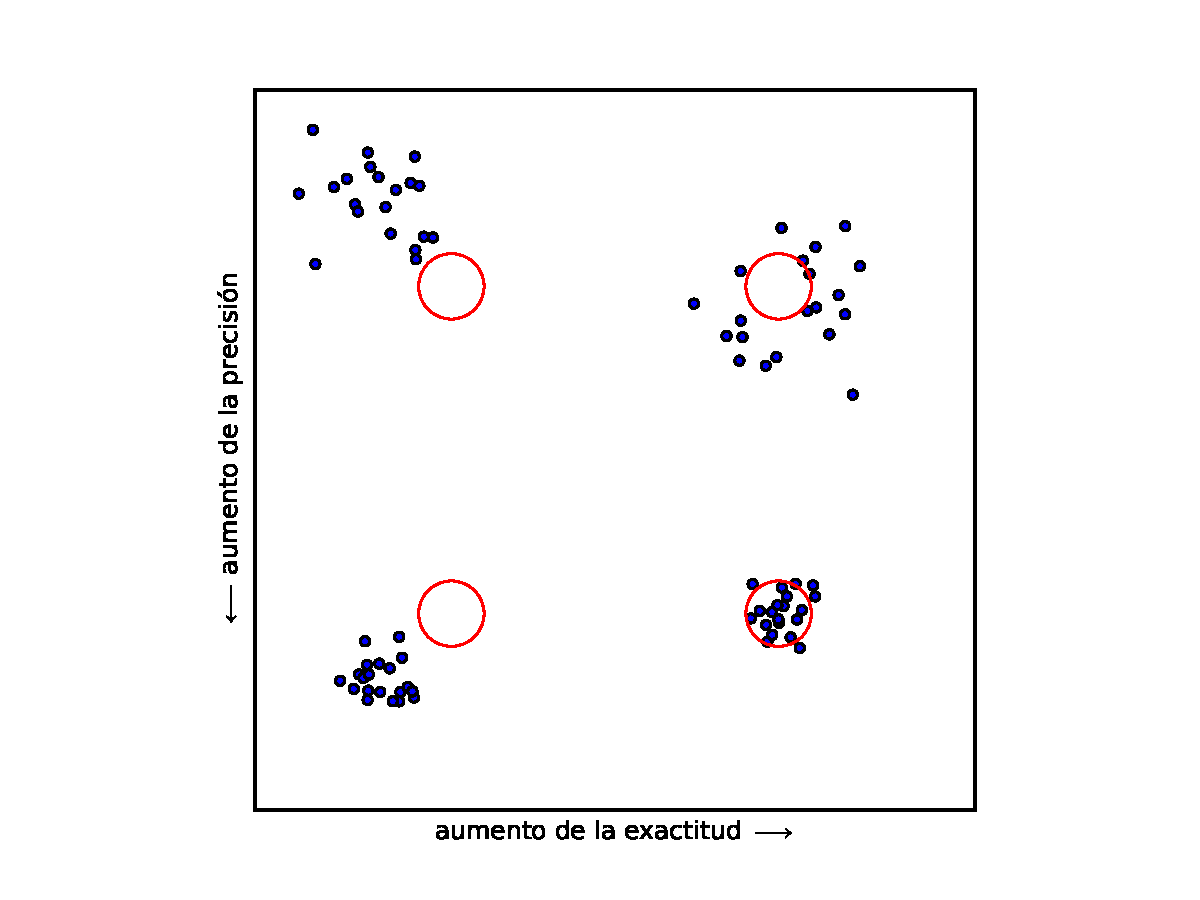
\includegraphics[width=12cm]{figs/fig-ex-vs-prec.pdf}
\caption{Exactitud versus precisi'on. C'odigo Python \href{https://github.com/gfrubi/Lab/blob/master/python/fig-ex-vs-prec.py}{aqu\'i}.}
\end{center}
\end{figure}

Asociado a los conceptos de precisi'on y exactitud est'a la idea de clasificar las fuentes de error en (al menos) tres tipos:
\begin{itemize}
\item \textbf{Error aleatorio}: La propiedad definitoria de los errores aleatorios es que 'estos producen resultados distintos al repetir una misma medici'on, incluso cuando se intentan dejar inalteradas todas las variables que determinan el resultado de 'este. Al repetir una medida varias veces, se obtienen diferentes resultados con una cierta dispersi'on. Esta dispersi'on determina entonces la precisi'on de los datos obtenidos. Como veremos, una medida de la dispersi'on de los datos, y por consiguiente de la precisi'on de la medida, es la \textbf{desviaci'on est'andar}. Las causas que producen el error aleatorio en un experimento son a menudo clasificadas como ``ruidos t'ecnicos"\, o ``ruidos fundamentales". Cada aparato tiene asociado un cierto l'imite de ruido fundamental determinado por la f'isica asociada a su funcionamiento. Sin embargo, usualmente el ruido t'ecnico es el dominante, y puede deberse a m'ultiples causas (mec'anicas, ambientales, variaciones en la forma en que se preparaci'on del sistema para repetir la medici'on... y un largo etc'etera!). Un(a) buen(a) f'isic@ experimental tiene experiencia y habilidad en identificar las posibles fuentes de ruido t'ecnico e idear formas de minimizarlo.

\item \textbf{Error sistem'atico}: Este tipo de error causa que los valores medidos se desplacen en alguna determinada direcci'on respecto al valor verdadero o aceptado. Por esto,  el error sistem'atico est'a relacionado con la exactitud del resultado: a mayor exactitud menor es el error sistem'atico. Las fuentes de este tipo de error pueden ser una defectuosa calibraci'on del instrumento de medici'on, o el uso de un m'etodo de medici'on que siempre sobre- o sub-estime la cantidad a determinar.

\item \textbf{Equivocaci'on}: Este tipo de error, en el que los m'etodos usados para estimar el error de una medida no son aplicables, se produce t'ipicamente porque alguna persona se equivoca en alguna de sus tareas. Por ejemplo, escribe mal el valor marcado en el instrumento al traspasarlo a su bit'acora (en papel, o en una planilla, o en un archivo con los datos, por ejemplo). Tambi'en puede ocurrir este tipo de error cuando la persona no ha chequeado correctamente la puesta en marcha de su instrumento, o que 'este est'e midiendo en una escala distinta, etc. etc. Si bien las equivocaciones pueden ser dif'iciles de distinguir de los errores sistem'aticos y aleatorios en la pr'actica, estos en principio no tienen relaci'on directa con el sistema f'isico, los instrumentos o el m'etodo usado, y en principio pueden ser eliminados repitiendo cuidadosamente el experimento.
\end{itemize}

En los gr'aficos de la figura \ref{fig-barras} se ilustra gr'aficamente las distintas posibilidades de error aleatorio y sistem'atico, por medio de \textbf{histogramas} (gr'aficos de barra de n'umero de ocurrencias de las medidas repetidas). En particular, suponemos que el valor verdadero de una variable es 10, y que medimos el valor de esta variable en repetidas oportunidades, para el caso simple en que nuestro instrumento nos suministre s'olo valores enteros.
\begin{figure}[h!]
\begin{center}
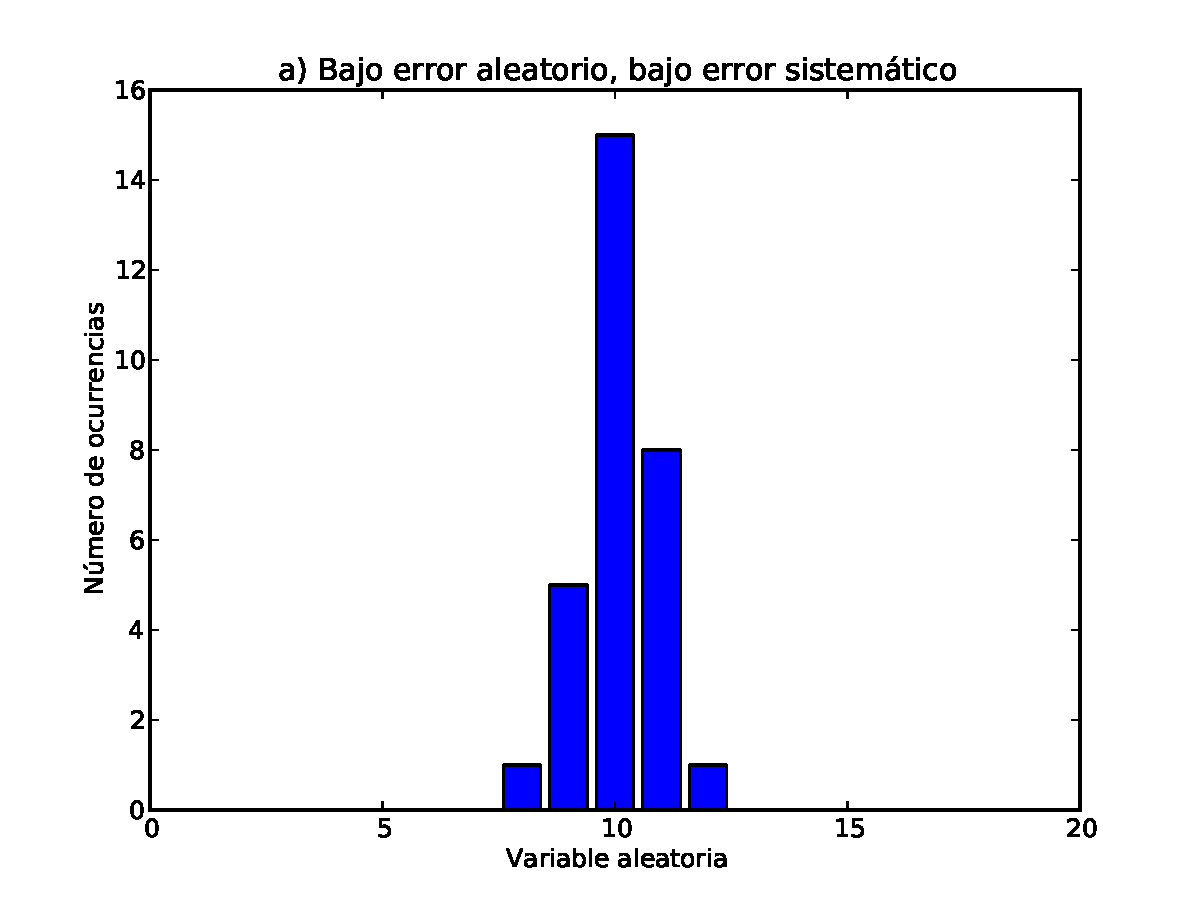
\includegraphics[width=7cm]{figs/fig-ba-bs.pdf}  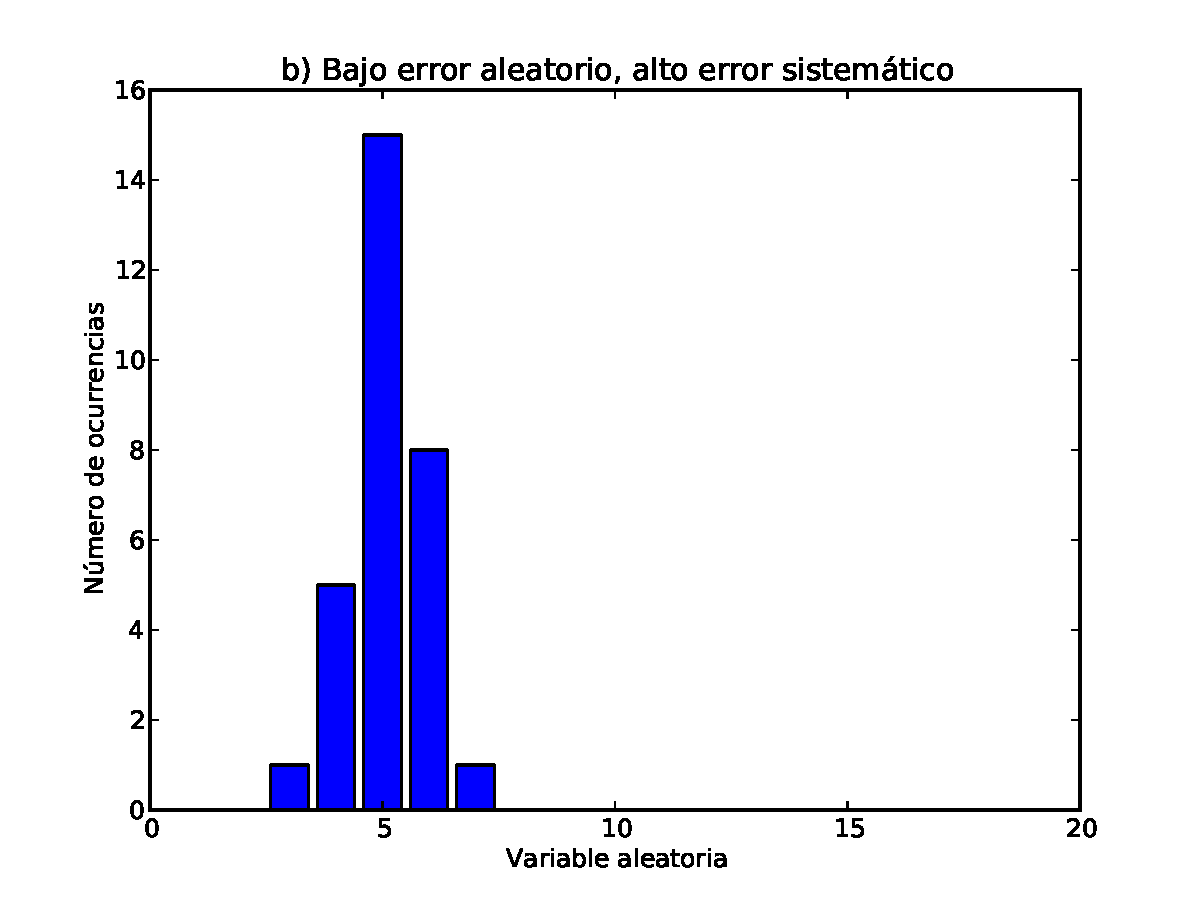
\includegraphics[width=7cm]{figs/fig-ba-as.pdf}
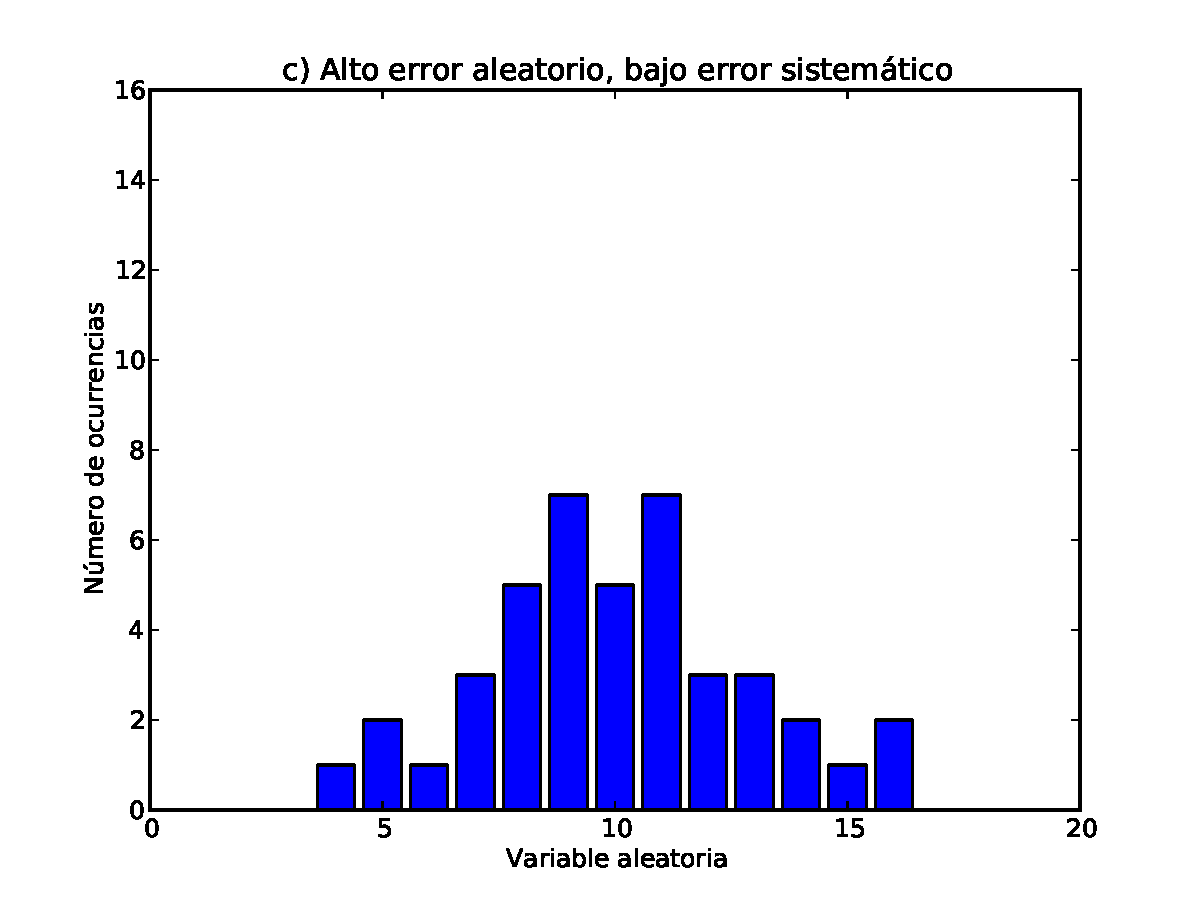
\includegraphics[width=7cm]{figs/fig-aa-bs.pdf}  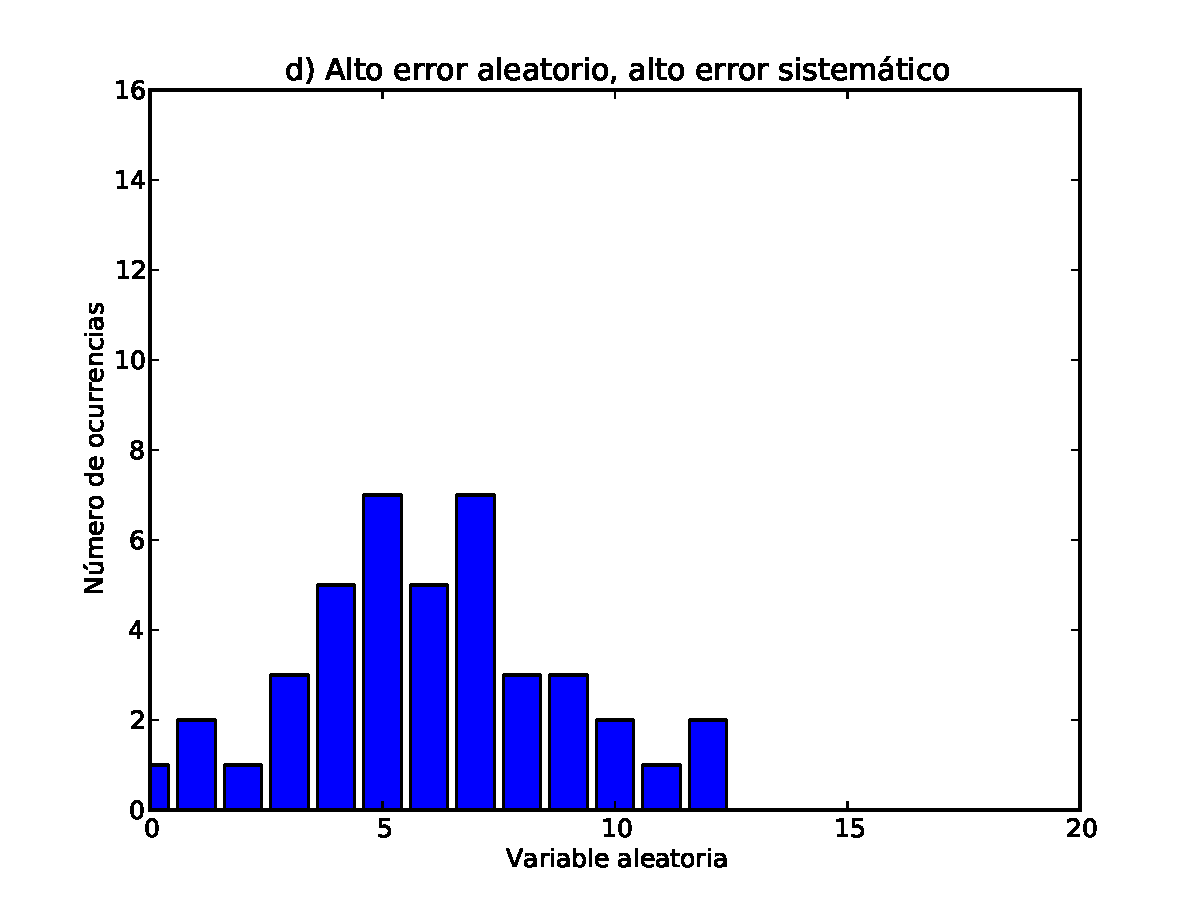
\includegraphics[width=7cm]{figs/fig-aa-as.pdf}
\caption{Distintas posibilidades para el tama\~no del error aleatorio y sistem'atico.  C'odigo Python \href{https://github.com/gfrubi/Lab/blob/master/python/fig-ba-bs.py}{aqu\'i}.}
\end{center}
\label{fig-barras}
\end{figure}


\section{Promedio y desviaci'on est'andar}

Cuando se realiza un experimento, generalmente se obtiene un conjunto de valores discretos $\lbrace x_i\rbrace$, $i=1,\dots,N$.  En el an'alisis de estos datos, a menudo son de gran utilidad los conceptos de \textbf{media}, \textbf{desviaci'on est'andar}, \textbf{varianza}, \textbf{error est'andar}, \textbf{suma residual de los cuadrados}  y la distribuci'on de los datos respecto del valor medio. 

La medida estad'istica m'as com'un es la \textbf{media}, definida como
\begin{equation}
\bar{x}:=\frac{1}{N}\sum_{i=1}^N x_i,
\end{equation}
donde $\lbrace x_i\rbrace$, $i=1,\dots,N$ representan los datos individuales y $N$ el n'umero total de 'estos.
Equivalentemente, podemos escribir
\begin{equation}
\bar{x}:=\frac{1}{N}\sum_{a=1}^{d} n_a x_a, \qquad N=\sum_{a=1}^{d} n_a,
\end{equation}
donde $n_a$ es el \textbf{n'umero de veces que se repite el valor} $x_a$ en la muestra y $d$ es el \textbf{n'umero de valores distintos} $\lbrace x_a\rbrace$, $a=1,\dots,d$.
%
%\begin{equation}
%\bar{y}:=\sum_{i=1}^N f_Y y_i,
%\end{equation}
%
%donde $ f_Y:= \frac{n_i}{N}$.
%
%\

La medida m'as com'un de la variabilidad de un conjunto de datos, es la \textbf{desviaci'on est'andar} respecto a la media:
\begin{equation}
s:=\sqrt{\frac{1}{N-1}\sum_{i=1}^N(x_i-\bar{x})^2}.
\end{equation}
Otro s'imbolo usando para la misma cantidad es $\sigma_{N-1}$, ver por ejemplo \cite{HH2010}. En Python, puede calcular la desviaci'on est'andar definida arriba usando la funci'on \texttt{std} de Numpy, con la opci'on \texttt{ddof=1}. Por ejemplo, \texttt{np.std(x, ddof=1)}.

Otro estimador de la variabilidad, el \textbf{error estándar}, es definido por:
\begin{equation}
\alpha:=\frac{s}{\sqrt{N}}.
\end{equation}
Si la dispersi'on de los datos respecto a la media aumenta, $s$, y $\alpha$ crecen. Por otro lado, si las medidas individuales est'an muy cerca del valor medio, estas cantidades ser'an menores. La dispersi'on tambi'en puede representarse por una magnitud llamada \textbf{varianza}, que por definici'on es el cuadrado de la desviaci'on est'andar,
\begin{equation}
s^2=\frac{1}{N-1}\sum_{i=1}^N(x_i-\bar{x})^2.
\end{equation}

 El valor del denominador, $N-1$ en lugar de $N$ se elige debido a que s'olo existen $N-1$ variaciones \textit{independientes} $(x_i-\bar{x})$, ya que $\sum_{i=1}^N (x_i-\bar{x})\equiv 0$. Formalmente decimos que se pierde un grado de libertad. Otra justificaci'on es que la dispersi'on no est'a definida en caso de tener s'olo un dato (en ese caso se obtiene $0/0$).

En t'erminos de los valores distintos $\lbrace x_a\rbrace$, y de su correspondiente n'umero de repeticiones $\lbrace n_a\rbrace$, podemos escribir la varianza como
\begin{equation}
s^2=\frac{1}{N-1}\sum_{a=1}^{d}n_a(x_a-\bar{x})^2.
\end{equation}

%Otra medida estad'istica que es 'util para cuantificar la dispersi'on es el \textbf{coeficiente de variaci'on}, definido por:
%\begin{equation}
%c.v.:=\frac{s}{\bar{x}}\times 100\%.
%\end{equation}
%
%\textbf{Suma residual}, es la suma de las diferencias al cuadrado entre el modelo predictor y los datos medidos.
%\begin{equation}
%\xhi^2:=\sum_{i=1}^N(y_i-f(x_i))^2.
%\end{equation}
%donde la funci'on $f(x_i)$ es el modelo usado para predecir los valores de $y_i$.


\section{Cifras significativas}

Al expresar una cierta magnitud f'isica, decimos que su valor tiene un cierto n'umero de \textbf{cifras significativas}, es decir, un cierto n'umero de d'igitos que, tomando en cuenta la incertidumbre en la determinaci'on de su valor, entregan informaci'on relevante del valor de la magnitud en cuesti'on. Las cifras significativas pueden t'ipicamente dividirse en cifras de las que se est'a completamente seguro, y en cifras que si bien no se tiene certeza absoluta de su valor, suministran informaci'on relavante para estimar el valor de la magnitud. Por ejemplo, la constante gravitacional en \eqref{G} fue expresada usando 6 cifras significativas ($6, 6, 7, 3, 8$ y $4$). Dada la incertidumbre en el valor de esta constante universal, s'olo las tres primeras cifras son seguras, mientras que las 'ultimas tres pueden cambiar. Sin embargo, en ese caso se ha considerado que las tres cifras no seguras tambi'en tienen informaci'on relavante de ser reportada. En general, no existe una regla absoluta y universamente aceptada sobre c'omo definir el n'umero de cifras significativas que es necesario o 'util de considerar al reportar un cierto resultado experimental. Por contraste, las siguientes reglas son univesalmente aceptadas para definir \textit{cifras que no son significativas}:
\begin{itemize}
\item Todos los ceros a la izquierda de una cantidad.
\item Ceros a la derecha de una cantidad, en el caso en que 'estos indican solamente la escala del n'umero (y/o las unidades de medida usadas).
\item Cifras espurias que aparezcan producto de c'alculos que van m'as all'a de la precisi'on que los datos originales determinan y que por este motivo no suministren ninguna informaci'on f'isicamente relevante de la magnitud.
\end{itemize}

En el caso en que un cero a la derecha de una cantidad se considere como significativo (es decir, que suministra informaci'on relavante, ya sea porque es una cifra segura o porque si bien no es segura es la cifra que se considera m'as probable) se acostumbra a escribir esa cifra expl'icitamente. Por ejemplo, si decimos que una distancia es $x_1=1,70{\rm\, km}$, estamos expresando que las cifras $1$ y $7$ y $0$ son significativas, mientras que si escribimos $x_2=1,7{\rm\, km}$ estamos indicando que s'olo 2 cifras son consideradas significativas. Si quieremos expresar las mismas cantidades, pero en unidades de metros y no kil'ometros, se acostumbra entonces escribir $x_1=1,70\times 10^3{\rm\, m}$ (3 cifras significativas) y $x_2=1,7\times 10^3{\rm\, m}$ (2 cifras significativas), respectivamente.

Ejemplos:

\begin{equation}
\begin{array}{ll}
2 & (1 \text{ cifra significativa)}\\
32 & (2 \text{ cifras significativas)}\\
12,470 & (5 \text{ cifras significativas)}\\
12,0010 &(6 \text{ cifras significativas)}\\
0,0023 & (2 \text{ cifras significativas)}\\
000156,210 & (6 \text{ cifras significativas)}\\
2,3\times 10^5 &(2 \text{ cifras significativas)}
\end{array}
\end{equation}


\subsubsection{Ejercicio}

Un(a) estudiante mide el largo de una mesa y como resultado nos entrega
la siguiente cantidad $(2,1\pm 0,5)$ m. Este(a) estudiante, por
conveniencia, decide expresar su resultado en mil'imetros. ?`C'omo tendr'ia
que expresar su resultado?, ?`$(2100\pm 50)$ mm?. \textbf{Resp.:} No, puesto que esto dar'ia a entender que la cantidad fue expresada con 4 cifras significativas, cuando en realidad s'olo tiene 2. La convenci'on para expresar el resultado es: $(2,1\pm 0,5)\times 10^3\,\rm mm$.

\section{Aproximaci'on y Redondeo}

Si queremos expresar el n'umero $\pi=3,14159265358979\cdots$ con $n$
cifras significativas, debemos desechar todas las cifras que se
encuentren a la derecha del en'esimo lugar. Adem'as, se adoptan las siguientes reglas para \emph{redondear} la $n$-'esima cifra:
\begin{enumerate}
\item Si la cifra que se encuentra en el lugar $(n + 1)$ es mayor que 5, se
  le agrega una unidad a la cifra que se encuentra en el lugar en'esimo.
\item Si la cifra que se encuentra en el lugar $(n + 1)$ es menor que 5,
  dejamos la cifra en'esima inalterable.
\item Si la cifra que se encuentra en el lugar $(n + 1)$ es igual a 5,
  adoptaremos la siguiente \textit{convenci'on}:
	\begin{itemize}
	\item Si la en'esima cifra es impar, se le agrega una unidad.
	\item Si la en'esima cifra es par la dejamos inalterable.
	\end{itemize}
Esta convenci'on intenta evitar la introducci'on del error sistem'atico que se agregar'ia si, por ejemplo, redondearamos siempre ``hacia arriba"\, la $n$-'esima cifra. En Python, estas reglas están implementadas en la función \texttt{round} de Numpy, ver \href{https://docs.scipy.org/doc/numpy/reference/generated/numpy.round_.html}{la documentaci\'on}.
\end{enumerate}

Note que estas convenciones de redondeo se aplican al valor principal de una magnitud f'isica y no al error asociado, puesto que este 'ultimo siempre se redondea a la cifra superior.

\section{Orden de magnitud}
Es la potencia de diez m'as cercana. 
Ejemplos:
\begin{itemize}
\item $6.7$ es de orden $10^1$ (est'a m'as cerca de 10 que de 1).
\item $5.3$ es de orden $10^0$ (est'a m'as cerca de 1 que de 10).
\item $128.9$ es de orden $10^2$ (est'a m'as cerca de 100 que de 1000).
\end{itemize}






\section{Precisi'on, sensibilidad, y cifras significativas}

En F'isica (y otras ciencias), estamos especialmente interesad@s en distinguir las cifras que son relevantes a la hora de expresar el resultado de una cantidad f'isica, de las que no lo son, \textit{a partir de la precisi'on con la que medimos o calculamos la cantidad} en cuesti'on. Por ejemplo, si medimos una 'unica vez el ancho de una hoja con una regla (o similar) que tiene una escala con una graduaci'on m'inima de un mil'imetro (decimos que la \textbf{sensibilidad del instrumento} es un 1\,mm), y vemos que el valor buscado est'a en la zona interior entre las marcas de la regla correspondientes a $21.5\,\rm cm$ y $21.6\,\rm cm$, podr'iamos expresar el resultado con 4 cifras significativas: $(21.55\pm 0.05)\,\rm cm$, o bien $(215.5\pm 0.5)\,\rm mm$. En este caso, la 'ultima cifra considerada como significativa es \textit{estimada}, es decir, aproximada por el criterio de la persona que realiza la medida. En este ejemplo, siendo conservadores (o pesimistas) aseguraremos que (con 100\% de confianza), el ancho de la hoja est'a comprendido en el intervalo entre $21.5\,\rm cm$ y $21.6\,\rm cm$ de modo que (en el peor de los casos) tendremos 2 cifras seguras ($2$ y $1$) y dos cifras que podr'ian variar, pero que nos entregan informaci'on f'isica relevante a la medici'on. Por el contrario, en este tipo de medici'on no tiene ning'un sentido f'isico reportar que el ancho de la hoja, medido con la misma regla, es $21.55275165359\,\rm cm$ puesto que las cifras $275165359$ no son para nada confiables (la cifra anterior, $5$, ya corresponde a una estimaci'on que realiz'o la persona que realiz'o la medida). En general, toda cifra que est'a m'as a la derecha de la posici'on que la precisi'on de la medida determina es considerada como no significativa (a menos que existen muy buenos argumentos para considerar lo contrario!).

Para estimar la precisi'on que determina (entre otras cosas) el n'umero de cifras significativas con las que se reporta un resultado o, equivalentemente el error o incertidumbre de la medida es 'util considerar varios casos:

\subsection{Caso de una 'unica medici'on}
En este caso se hace, a su vez, la distinci'on entre:
\begin{itemize}
\item \textbf{Medici'on realizada con un instrumento anal'ogico}: Aqu'i decimos que la sensibilidad del instrumento es el valor de la m'inima subdivisi'on en la escala que 'este posee. Para la regla considerada en el ejemplo anterior, decimos que su sensibilidad es 1\,mm. Es razonable considerar la incertidumbre o error de una medida realizada con un instrumento anal'ogico como la mitad del valor de su sensibilidad: 0.5\,mm en el caso de la regla. Esta es la ``elecci'on conservadora''\, para el error de la medida\footnote{En algunas ocasiones, sin embargo, esta elecci'on puede ser claramente demasiado pesimista. Considere por ejemplo que se mide el mismo ancho de la hoja, pero con una regla que tenga una sensibilidad de 1\,cm (la menor graduaci'on marcada en ella). En este caso la medida quedar'a entre 21\,cm y 22\,cm, y el error ``conservador''\, asociado ser'ia de $\pm 0.5\,\rm cm$, pudiendo expresar el resultado como $(21.5\pm 0.5)\rm cm$ que, al ojo humano sano, puede parecer muy pesimista. Un(a) f'isic(a) experimental con experiencia y habilidad podr'ia ser capaz de realizar una mejor estimaci'on de la 'ultima cifra y acotar el error asociado asegurando, por ejemplo, que el ancho est'a entre $21.1\,\rm cm$ y $21.7\,\rm cm$ y por lo tanto informe que $(21.4\pm 0.3)\rm cm$. Dado que no existe una receta general y 100\% aceptada de c'omo proceder en estos casos (que aseguren que las personas que reciben el resultado tengan confianza en 'el), adoptaremos aqu'i la postura ``pesimista'', es decir, consideraremos que el error de una medici'on es igual a la mitad de la sensibilidad del instrumento.}

\item \textbf{Medici'on realizada con un instrumento digital}: Suponga que mide el mismo ancho de la hoja, pero ahora usando un instrumento digital\footnote{?`C'omo podr'ia hacer esto?, ?`Con qu'e instrumento?}), que suministra valores discretos en una pantalla, por ejemplo ``21.57''\,cm. ?`Qu'e error asociamos a la medida?. Nuevamente, la respuesta no es 'unica, puesto que depende de c'omo exactamente funciona el dispositivo, y de c'omo realiza el redondeo y/o truncamiento de cifras que finalmente son mostradas en la pantalla. Algunos instrumentos digitales traen consigo especificaciones t'ecnicas del fabricante que establecen que el error debe considerarse como ``la mitad del 'ultimo d'igito''\,. En nuestro ejemplo reportar'iamos entonces que el ancho es $(21.570\pm 0.005)\rm cm$ (el 'ultimo 0 ser'ia una cifra significativa en este caso) o, equivalentemente, que el valor est'a en el intervalo entre $21.565\,\rm cm$ y $21.575\,\rm cm$. Como podemos ver, este caso requiere que el instrumento (internamente) \textbf{redondee} (aproxime) el valor de la medida, y que no simplemente \textbf{trunque} (corte) el valor. En el caso que se desconozcan los detalles t'ecnicos del instrumento y/o si 'este aproxima o trunca las cifras es preferible, nuevamente, adoptar la postura ``conservadora''\, y considerar como error de la medida a la unidad correspondiente al 'ultimo d'igito que el instrumento indica. En nuestro ejemplo, $\pm 0.01\rm cm$, y reportar que $(21.57\pm 0.01)\rm cm$.
\end{itemize}

\subsection{Caso de mediciones repetidas}

En este caso, es necesario a recurrir a herramientas estad'isticas para caracterizar algunos aspectos de la precisi'on de los resultados, puesto que es esencial tomar en cuenta que se realizan varias (idealmente, muchas) medidas, y que 'estas en general no arrojar'an los mismos valores, por lo que los datos estudiados tendr'an cierta dispersi'on. Existen distintas cantidades que son 'utiles para caracterizar el valor caracter'istico y la dispersi'on en los datos, pero que necesariamente reducen la riqueza y complejidad 'estos. Teniendo esto en cuenta, es posible usar (por ejemplo) el promedio ($\bar{x}$) y la desviaci'on est'andar ($\sigma$) (es decir, s'olo dos valores!) para expresar el valor caracter'istico y el ``error'' de una magnitud f'isica que queremos determinar a partir de muchas medidas individuales. Hay, sin embargo, un precio que pagar: es necesario incluir adem'as un valor para la \textbf{probabilidad de que el valor buscado est'e dentro de cierto intervalo} (por ejemplo, $\bar{x}\pm \sigma$).

\section{Propagaci'on de incertezas}

Inevitablemente, siempre que calculemos una magnitud f'isica a partir de otras sujetas a incerteza/error, 'esta incerteza se propagar'a a la cantidad calculada. Existen varias formas de calcular la incerteza de la magnitud calculada a partir de la expresi'on anal'itica que la define y de  incertezas de las magnitudes originales. Si la relaci'on es simple es posible encontrar expresiones anal'iticas exactas para el error propagado. En otros casos tambi'en es posible encontrar expresiones anal'iticas aproximadas cuando el error de las magnitudes originales es suficientemente peque\~no. Actualmente es tambi'en muy com'un evaluar num'ericamente el error propagado, puesto que este m'etodo puede ser usado cuando la relaci'on entre las variables en muy complicada y adem'as cuando el error no necesariamente es peque\~no.

Un caso simple donde es posible encontrar una expresi'on anal'itica exacta para el error propagado es en el caso de la suma y resta de dos magnitudes:
\begin{itemize}
\item \textbf{Suma:} Si $y=x_1+x_2$, $x_1 = \bar{x}_1\pm\Delta x_1$ y $x_2 = \bar{x}_2\pm\Delta x_2$, entonces
\begin{equation}
\bar{y}= \bar{x}_1+\bar{x}_2, \qquad  \Delta y= \Delta x_1+\Delta x_2.
\end{equation}
\item \textbf{Resta:} Si $y=x_1-x_2$, entonces
\begin{equation}
\bar{y}= \bar{x}_1-\bar{x}_2, \qquad  \Delta y = \Delta x_1+\Delta x_2.
\end{equation}
\end{itemize}

En el caso de la multiplicaci'on y divisi'on la situaci'on es menos simple:
\begin{itemize}
\item \textbf{Multiplicaci'on:} Si $y=x_1 x_2$, (y suponiendo $x_1$ y $x_2$ positivos)
\begin{equation}
y_{\rm min} = (\bar{x}_1-\Delta x_1)(\bar{x}_2-\Delta x_2), \qquad 
y_{\rm max} = (\bar{x}_1+\Delta x_1)(\bar{x}_2+\Delta x_2).
\end{equation}
Vemos aqu'i que el punto medio no coincide con el valor que se obtendr'ia sin considerar el error, ya que
\begin{equation}
\frac{1}{2}\left(y_{\rm min}+y_{\rm max}\right) = \bar{x}_1\bar{x}_2+\Delta x_1\Delta x_2,
\end{equation}
en otras palabras, el intervalo $[y_{\rm min},y_{\rm max}]$ no es sim'etrico respecto a $\bar{x}_1\bar{x}_2$.

Esta asimetr'ia puede ignorarse si los errores relativos de $x_1$ y $x_2$ son suficientemente peque\~nos, de modo que $u_r^{x_1}\ll 1$ y $u_r^{x_2}\ll 1$. En este caso,
\begin{equation}
\frac{1}{2}\left(y_{\rm min}+y_{\rm max}\right) \approx \bar{x}_1\bar{x}_2,
\end{equation}
y podemos expresar el valor de $y$ como $\bar{y}\pm\Delta y$, con
\begin{equation}
\bar{y} \approx \bar{x}_1\bar{x}_2, \qquad  \Delta y= x_2\Delta x_1 + x_1\Delta x_2 , 
\end{equation}
o, equivalentemente,
\begin{equation}
u_r^{y} \approx u_r^{x_1} + u_r^{x_2}.
\end{equation}

\item \textbf{Divisi'on:} Si $y=x_1/x_2$, y suponiendo $x_1$ y $x_2$ positivos, tendremos una situaci'on similar. Los valores extremos estar'an dados por
\begin{equation}
y_{\rm min} = \frac{\bar{x}_1-\Delta x_1}{\bar{x}_2+\Delta x_2}, \qquad 
y_{\rm max} = \frac{\bar{x}_1+\Delta x_1}{\bar{x}_2-\Delta x_2},
\end{equation}
por lo que el valor medio y el ancho del intervalo son dados por
\begin{equation}
\frac{1}{2}\left(y_{\rm min}+y_{\rm max}\right) = \frac{\bar{x}_1\bar{x}_2+\Delta x_1\Delta x_2}{\bar{x}_2^2-(\Delta x_2)^2}, 
\qquad \frac{1}{2}\left(y_{\rm max}-y_{\rm min}\right) = \frac{\bar{x}_2\Delta x_1 + \bar{x}_1\Delta x_2}{\bar{x}_1^2-(\Delta x_1)^2}.
\end{equation}
El punto medio s'olo coincide aproximadamente con el valor $\bar{x}_1/\bar{x}_2$ si el error (relativo) es muy peque\~no. Suponiendo que esto es cierto, podremos escribir $y = \bar{y}\pm\Delta y$, con
\begin{equation}
\bar{y}\approx \frac{\bar{x}_1}{\bar{x}_2}, \qquad  \Delta y \approx \frac{1}{x_2}\Delta x_1 + \frac{x_1}{x_2^2}\Delta x_2
\end{equation}
o, equivalentemente,
\begin{equation}
u_r^{y} \approx  u_r^{x_1} + u_r^{x_2}.
\end{equation}

\item \textbf{Potencias:} Es simple generalizar los resultados anteriores al caso en que $y=x_1^{\alpha_1} x_2^{\alpha_2}$, el intervalo de valores posibles de $y$ tampoco ser'a sim'etrico respecto al valor calculado sin tomar en cuenta los errores de cada variable: $\bar{y}=\bar{x}_1^{\alpha_1}\bar{x}_2^{\alpha_2}$. Sin embargo, en el caso en que los errores relativos satisfagan $u_r^{x_1}\ll 1$ y $u_r^{x_2}\ll 1$ podremos escribir
\begin{equation}
\bar{y}\approx \bar{x}_1^{\alpha_1}\bar{x}_2^{\alpha_2}, \qquad  u_r^{y} \approx  |\alpha_1|u_r^{x_1} + |\alpha_2|u_r^{x_2}.
\end{equation}
\end{itemize}


\paragraph{Ejemplo:}
 Suponga que determinamos el volumen de un gas a partir de la ecuaci'on para un gas ideal,
\begin{equation}
V(p,T,n,R)=\frac{nRT}{p},
\end{equation}
donde cada magnitud f'isica es medida con su respectivo error asociado:
\begin{equation}
p=(100\pm 3)\times 10^3\text{ Pa}, \quad T=(300.0\pm 0.2)\text{ K}, 
\quad n=(0.10\pm 0.01)\text{ mol},
\end{equation}
mientras que de una tabla de datos se obtiene
\begin{equation}
R=(8.31\pm 0.01)\text{ J/mol K}.
\end{equation}
El valor principal del volumen:
\begin{equation}
\bar{V}= V(\bar{p},\bar{T},\bar{n},\bar{R}) \approx 0.002493\text{ m}^3.
\end{equation}
Ahora evaluaremos el error relativo asociado con el volumen, usando
\begin{align}
u_r^V &\approx u_r^n+ u_r^R + u_r^T + u_r^p \\
&\approx \frac{0.01}{0.1} + \frac{0.01}{8.31} + \frac{0.2}{300} + \frac{3}{100} \\
&\approx 0.1 + 0.0012 + 0.00067 + 0.03 \\
&\approx 0.132.
\end{align}
Con esto, el error absoluto $\Delta V$ queda determinado por
\begin{equation}
\Delta V = \bar{V}u_r^V \approx (0.002493\text{ m}^3)(0.13) \approx 3.3\times 10^{-4}\text{ m}^3.
\end{equation}
Tomando en cuenta el error calculado, expresamos el resultado final truncando el valor de $\bar{V}$ de acuerdo a las reglas antes descritas:
\begin{equation}
 V \approx (0.002493\pm 0.00033)\text{ m}^3 \approx (2.49\pm 0.33)\times 10^{-3}\text{ m}^3.
 \end{equation} 

\paragraph{Ejemplo:}
Supongamos que queremos medir el periodo de un p'endulo y, medimos el tiempo que tarda en hacer 10 oscilaciones, con un cron'ometro (digital) de sensibilidad $0.1\,\rm s$. Si el tiempo total es de $t=(4.6\pm 0.1)\,\rm s$, tendremos que el periodo medio es 
\begin{equation}
\bar{P} = \frac{\bar{t}}{10}=\frac{4.6\,\rm s}{10}=0.46{\,\rm s}.
\end{equation}
Y el error puede ser estimado usando
\begin{equation}
\Delta P = \frac{0.1\,\rm s}{10}=0.01{\,\rm s},
\end{equation}
de modo que
\begin{equation}
P=(0.46\pm 0.01){\,\rm s}.
\end{equation}

Note que por el solo hecho de haber medido el tiempo de 10 oscilaciones consecutivas y haber calculado a partir de 'este el tiempo de una 'unica oscilaci'on parece que hemos aumentado la precisi'on de la medida, tal como si us'aramos un instrumento 10 veces m'as sensible. Si bien este m'etodo es apropiado y usado en muchas ocasiones, existe un ``precio que pagar'' por este aumento efectivo de la precisi'on: \textit{hemos supuesto que el periodo de oscilaci'on del p'endulo durante las 10 oscilaciones permanece inalterado}. Esta es una hip'otesis f'isica adicional introducida, que puede o no ser cierta. En otras palabras, si el periodo de oscilaci'on del p'endulo no permanece constante durante las 10 oscilaciones, la cantidad calculada es simplemente el valor promedio de los periodos y no necesariamente el valor que se busca determinar.

\paragraph{Ejemplo:}
La ley de gravitaci'on universal de Newton, determina la fuerza $\vec{F}$ entre dos masas (muy peque\~nas) $m_1$ y $m_2$ separadas por una distancia $d$, de modo que $
F=G{m_1m_2}/{d^2}$. En un experimento se quiere determinar la constante gravitacional con un error relativo $u_G\approx 10^{-3}$, usando 
\begin{equation}
G=\frac{Fd^2}{m_1m_2}.
\end{equation}
Para esto, se ubican dos masas iguales $m_1=m_2=(100{\,\rm kg}\pm 1{\,\rm g})$ a una distancia $d\approx 0.5{\, \rm m}$, y se mide la fuerza entre las masas, con un error relativo $u_F=2\times 10^{-4}$. Determine el error absoluto con el que deben medirse la distancia $d$ que el error relativo de $G$ sea el deseado.

\textbf{Soluci'on:} En este caso, los errores relativos conocidos son mucho menores que 1, ya que
\begin{equation}
u_r^F =2\times 10^{-4}, \qquad u_r^m = \frac{1\,\rm g}{100\,\rm kg}  = 10^{-5}, \qquad u_r^G\approx 10^{-3},
\end{equation}
de modo que podemos usar la expresion aproximada para el error relativo propagado:
\begin{equation}
u_r^G \approx u_r^F + 2u_r^d + 2u_r^m.
\end{equation}
Despejando $u_r^d$, obtenemos
\begin{align}
u_r^d &\approx \frac{1}{2}\left(u_r^G - 2u_r^F - 2u_r^m\right) \\
& \approx\frac{1}{2}\left(10^{-3} - 4\times 10^{-4} - 2\times 10^{-5}\right) \\
& \approx 4\times 10^{-4}.
\end{align}
El valor del error absoluto de las medidas de $d$ debe entonces ser aproximadamente de $\Delta r = r\cdot u_r^r \approx (0.5 m)(4\times 10^{-4})\approx 0.2\,\rm mm$.

\subsection{Funciones arbitrarias y error suficientemente peque\~no}

Si $y=y(x)$, y $x=\bar{x}\pm \Delta x$ entonces
\begin{equation}
\Delta y \approx \Delta x \left|\frac{dy}{dx}(\bar{x})\right|.
\end{equation}

Si $y=y(x_1,x_2,\dots,x_m)$, y $x_\alpha=\bar{x}_\alpha\pm \Delta x_\alpha$, $\alpha=1,\dots, m$ entonces
\begin{equation}
\Delta y \approx \sum_{\alpha=1}^m\Delta x_\alpha \left|\frac{\partial y}{\partial x_\alpha}(\bar{x}_1,\dots,\bar{x}_m)\right|.
\end{equation}

\subsection{Evaluaci'on num'erica}

\chapter{Ajuste de curvas}

\section{Modelos de regresi'on}

Generalmente, al realizar un experimento se obtiene como resultado un conjunto de puntos discretos y, como ya hemos mencionado, en muchas ocasiones se requiere modelar la \textit{dependencia funcional} entre dichos puntos. En otras ocasiones se requieren puntos \textit{entre} esos valores discretos. Para lograr algunos de estos objetivos se requiere de \textbf{t'ecnicas de ajuste de curvas} tanto para obtener valores intermedios como para determinar la forma en que se relacionan dichas variables. 
Otras veces, lo que se busca es una expresi'on simplificada de una funci'on muy complicada, que se ajuste bien en alg'un rango deseado. Para encontrar esta funci'on simplificada, suele evaluarse la funci'on m'as complicada para varios puntos y tratar estos puntos con el mismo criterio de ajuste que los datos obtenidos experimentalmente.
 
Las t'ecnicas de ajuste las separaremos en dos grupos generales:
\begin{enumerate}
\item Cuando los datos obtenidos muestran imprecisi'on, es decir un grado significativo de error aleatorio (ruido) y lo que se busca es determinar la \textit{tendencia} y no necesariamente un modelo que describa detalladamente cada variaci'on sistem'atica de los datos experimentales.

La estrategia aqu'i es encontrar una curva, dentro de una familia dada, que represente el comportamiento general, es decir, ajustar un modelo. Dicho modelo no necesariamente interceptar'a cada uno de los  puntos. No debemos olvidar que estamos estudiando el caso donde los datos presentan ruido y por este motivo es que no podemos considerar cada punto de manera individual, ya que 'este podr'ia ser incorrecto. Con este criterio de b'usqueda nos queda claro que el modelo (la dependencia funcional entre las variables) que deseamos encontrar debe describir el patr'on del conjunto de puntos o datos experimentales. Para este caso usaremos un \textbf{modelo de regresi'on}.

\item Cuando los datos obtenidos muestran una gran precisi'on o un grado m'inimo de error aleatorio (poco ruido) y lo que se desea determinar son valores entre datos experimentales sin estar interesados en modelar el fen'omeno, es decir, no se est'a buscando la dependecia entre las variables involucradas.
 
	En este caso, tenemos como objetivo encontrar una curva o una serie de curvas que pasen exactamente por cada uno de los puntos. La diferencia fundamental con el caso anterior es que cada punto se considera como correcto. 
	
A la estimaci'on de valores entre puntos discretos se le conoce con el nombre de \textbf{interpolaci'on}.
\end{enumerate}

\begin{figure}[h!]
\begin{center}
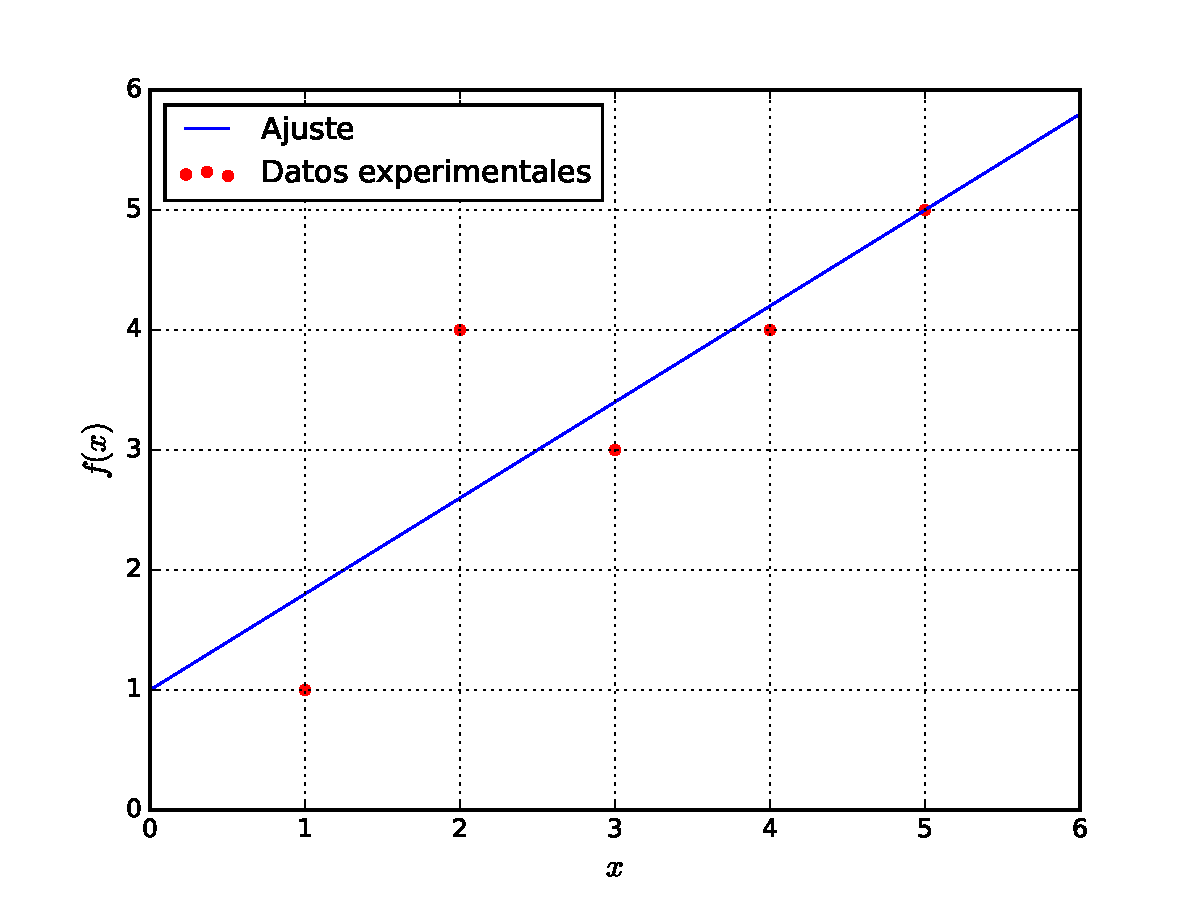
\includegraphics[width=10cm]{figs/fig-mmc.pdf}\label{intmc}
\caption{Ajuste lineal. C'odigo Python \href{https://github.com/gfrubi/Lab/blob/master/python/fig-mmc.py}{aqu\'i}.}
\end{center}
\end{figure}

\begin{figure}[h!]
\begin{center}
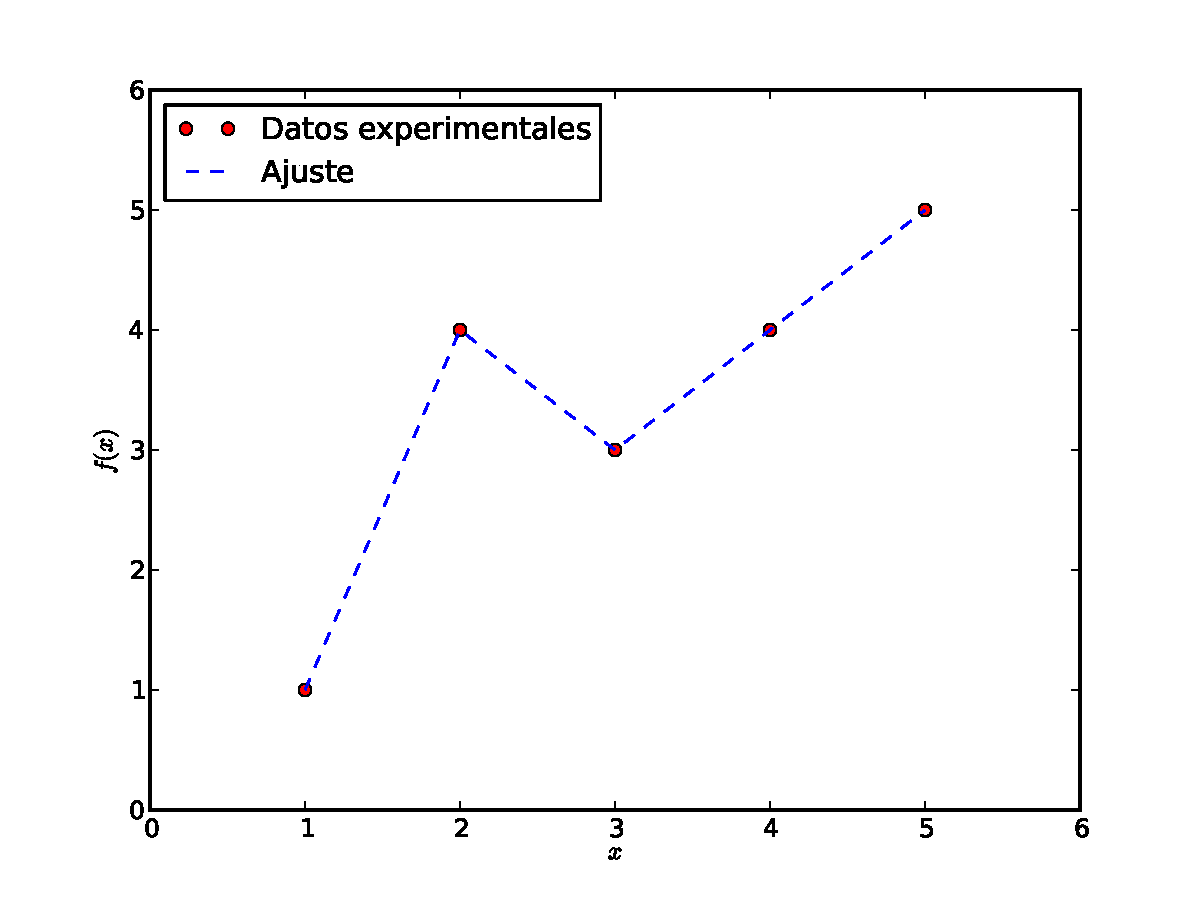
\includegraphics[width=10cm]{figs/fig-int-lineal.pdf}\label{intil}
\caption{Interpolaci'on lineal. C'odigo Python \href{https://github.com/gfrubi/Lab/blob/master/python/fig-int-lineal.py}{aqu\'i}.}
\end{center}
\end{figure}

\begin{figure}[h!]
\begin{center}
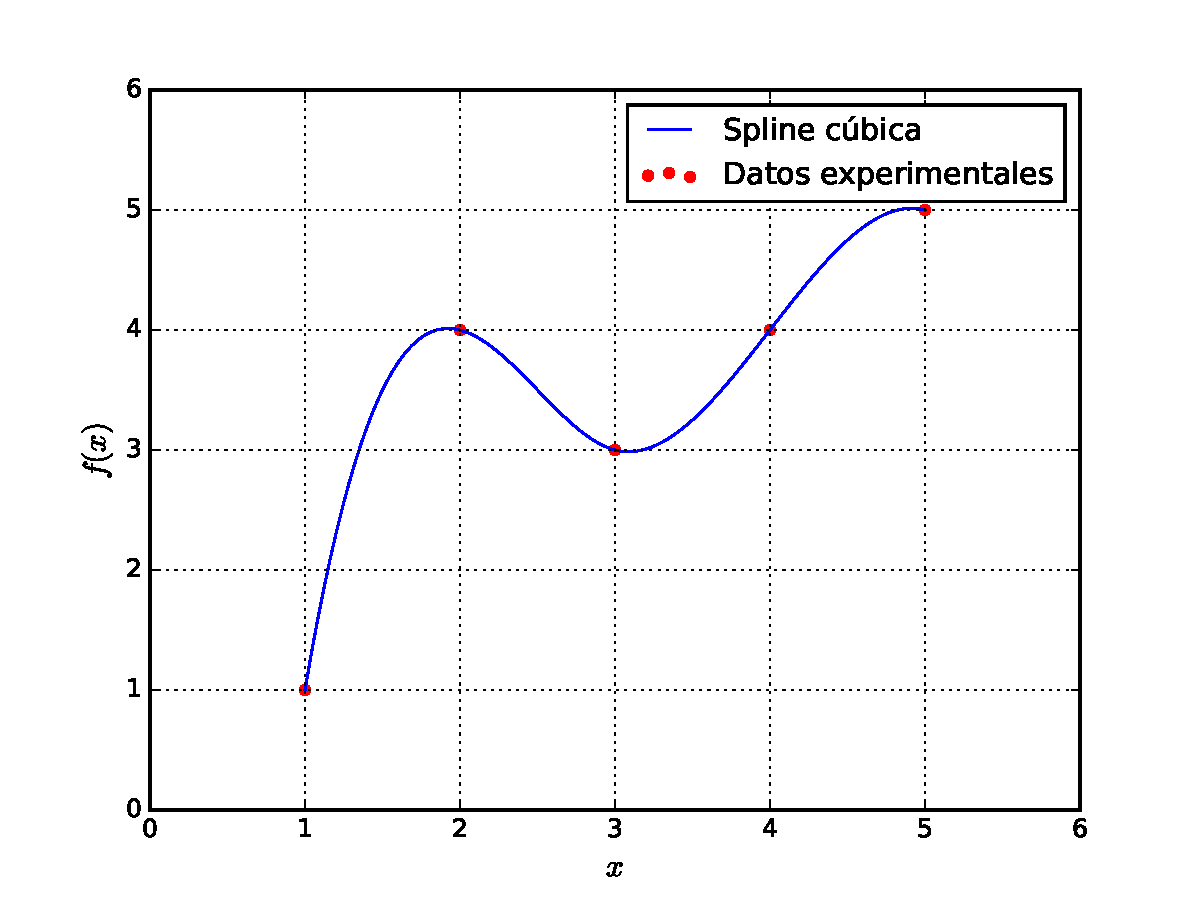
\includegraphics[width=10cm]{figs/fig-int-curv.pdf}\label{intic}
\caption{Interpolaci'on spline c'ubica. C'odigo Python  \href{https://github.com/gfrubi/Lab/blob/master/python/fig-int-curv.py}{aqu\'i}.}
\end{center}
\end{figure}

Suponga que se obtiene experimentalmente un conjunto de datos que son presentados en las figuras \ref{intmc}-\ref{intic}.

El primer intento de ajuste (ver fig. \ref{intmc}), no pretende conectar los puntos, s'olo trata de caracterizar el crecimiento de los datos mediante una l'inea recta. Esta t'ecnica ofrecer'ia una estimaci'on adecuada solamente para el caso lineal. Para el segundo caso (ver fig. \ref{intil}) se utilizaron segmentos rectos entre cada par de puntos, es decir, una \textbf{interpolaci'on lineal} que conecta dichos puntos.  Esta t'ecnica, ofrecer'ia una estimaci'on adecuada solamente para el caso donde los puntos est'an muy cercanos unos de otros y cada uno de ellos hubiese sido medido con un error aleatorio m'inimo, tal que cada punto sea significativo.

Sin embargo, cuando la relaci'on subyacente es altamente no-lineal o cuando los datos est'an muy separados entre si, se pueden introducir errores importantes al realizar una interpolaci'on lineal. En el tercer caso (ver fig. \ref{intic}) se usaron curvas que intentan capturar el comportamiento general de los datos. Este criterio para ajustar la curva ser'a el adecuado si cada uno de los puntos del conjunto de datos est'a medido con un error suficientemente grande tal que el conjunto nos de informaci'on del comportamiento general, pero no cada uno de los puntos individualmente.

Lo comentado deja de manifiesto la necesidad de desarrollar m'etodos sistem'aticos y objetivos con el prop'osito de determinar la curva m'as adecuada, ya sea para modelar o interpolar.

El \textbf{an'alisis de tendencias} representa el proceso de usar el patr'on de los datos y hacer predicciones, pudi'endose usar polinomios de interpolaci'on para el caso en que los datos fueron tomados con alta precisi'on. Este tipo de an'alisis se usa para predecir valores de la variable dependiente, \textbf{interpolaciones} (predecir dentro del rango de datos medidos).
Otra de las aplicaciones del ajuste de curvas experimentales consiste en poner a prueba hip'otesis. Esto consiste en comparar nuestro modelo te'orico con los valores medidos. Pudiendo a veces ajustar los coeficientes desconocidos del modelo para que 'este se ajuste mejor al experimento.

Finalmente, estos m'etodos de ajuste pueden usarse para derivar funciones simples que se aproximen, dentro de un rango, a funciones complicadas.

\section{Regresi'on Lineal Simple}

Este modelo considera s'olo una variable independiente $x$ y una variable dependiente $y$, y supone que la relaci'on subyacente entre la variable independiente y dependiente es lineal, es decir,
\begin{equation}
y =\alpha_0 + \alpha_1 x,
\end{equation}
donde el coeficiente de posici'on $\alpha_0$ y la pendiente $\alpha_1$ son los coeficientes desconocidos de la regresi'on. 

Por otro lado, supongamos que cada una de las observaciones de $Y$ quede descrita por el siguiente modelo
\begin{equation}
y_i=  \alpha_0 + \alpha_1 x_i +\epsilon_i
\end{equation}
donde $\epsilon_i$ son los residuos de la regresi'on y son interpretados como un \textit{error aleatorio} (valores no correlacionados) con valor medio igual a cero.
% y varianza constante $\sigma^{2}$, es decir, $V(\epsilon_i)=\sigma^{2}$. Entenderemos que la varianza es constante cuando para un $x_i$ dado, la variabilidad en $y_i$ queda descrita por un mismo  $\sigma^{2}$ para todos los elementos de la muestra aleatoria. 

A partir de un conjunto de datos experimentales (una muestra) podemos hacer estimaciones $a_0$ y $a_1$ de los coeficientes $\alpha$ y $\alpha_1$.
Un m'etodo com'unmente usado para estimar dichos par'ametros es el \textbf{m'etodo de m'inimos cuadrados}. 
%
%Si tenemos una muestra aleatoria formada por $N$ pares de observaciones $\{(x_{1},y_{1}),(x_{2},y_{2}),\dots ,(x_{N},y_{N}) \}$ y proponemos un modelo lineal $y=b_0 + b_1 x$ para caracterizar el comportamiento de los datos experimentales, es posible expresar cada par de observaciones como
%\begin{equation}
%y_{i}=b_0 + b_1 x_{i} +\epsilon_{i},\qquad	i=1,2, \dots, N.
%\end{equation}

La suma de los cuadrados de las diferencias entre los datos medidos y la predicción realizado por el modelo propuesto (o \textbf{residuos}) est'a dada por
\begin{equation}
\chi^2(a_0,a_1)= \sum_{i=1}^N\epsilon_{i}^{2}= \sum_{i=1}^N (y_{i} - a_0 - a_1 x_{i})^{2}.
\end{equation}

Minimizando la suma de los cuadrados con respecto a los coeficientes desconocidos, obtenemos los estimadores $a_0$ y $a_1$ de los par'ametros $\alpha_0$ y $\alpha_1$. Las ecuaciones que determinan los estimadores son

\begin{equation}\label{dchi2db0}
\frac{\partial \chi^2}{\partial a_0}=-2 \sum_{i=1}^N (y_{i} - a_0 - a_1 x_{i})=0,
\end{equation}

\begin{equation}
\frac{\partial \chi^2}{\partial a_1}=-2 \sum_{i=1}^N (y_{i} - a_0 - a_1 x_{i})x_i=0.
\end{equation}
Simplificando y reordenando t'erminos, obtenemos:
\begin{equation}
N a_0 + a_1\sum_{i=1}^N x_{i}=\sum_{i=1}^N y_{i},
\end{equation}
\begin{equation}
a_0\sum_{i=1}^N x_{i}  + a_1\sum_{i=1}^N x_{i}^{2}=\sum_{i=1}^N y_{i}x_{i},
\end{equation}
\begin{equation}
\left( \begin{array} {cc}
N&\sum_{i=1}^N x_{i} \\  \\
\sum_{i=1}^N x_{i}&\sum_{i=1}^N x_{i}^{2} 
 \end{array}\right) \left( \begin{array} {c}
 a_0 \\  \\
 a_1 
  \end{array}\right)=\left( \begin{array} {c}
   \sum_{i=1}^N x_{i} \\  \\
   \sum_{i=1}^N y_{i}x_{i} 
    \end{array}\right).
\end{equation}

Resolviendo el sistema se obtiene
\begin{equation}
a_0 = \bar{y}-a_1 \bar{x},
\end{equation}
\begin{equation}
a_1 =  \frac{N\left(\sum_{i=1}^N y_{i}x_{i}\right)-\left(\sum_{i=1}^N y_{i}\right)\left(\sum_{i=1}^N x_{i}\right) }{N\left(\sum_{i=1}^N x_{i}^{2}\right)- \left(\sum_{i=1}^N x_{i}\right)^{2}}=\frac{\overline{xy}-(\bar{x})(\bar{y})}{\overline{x^2}-(\bar{x})^2},
\end{equation}
donde $\bar{x}$, $\bar{y}$, $\overline{xy}$ y $\overline{x^2}$ representan los promedios de $\{x_i\}$, $\{ y_i\}$, $\{x_iy_i\}$ y $\{x_i^2\}$ respectivamente. 

Una manera de cuantificar la dispersi'on de los datos en torno del modelo es calcular la desviaci'on est'andar
\begin{equation}
S_{Y/x} = \sqrt{\dfrac{S_{r}}{N-2}},
\end{equation}
con 
\begin{equation}
S_{r}= \sum_{i=1}^N (y_{i} - a_0 - a_1 x_{i})^{2}.
\end{equation}

Note que para ajustar el modelo se introdujeron dos valores medios, es decir, se perdieron dos grados de libertad. Otra justificacion del t'ermino $N-2$ en el c'alculo de la varianza es que si ajustamos una recta para s'olo dos puntos no habr'ia dispersi'on.


Adem'as, el \textit{coeficiente de determinaci'on} $r^2$ es definido por
\begin{equation}\label{r2}
r^2 = \dfrac{S_{t} - S_{r}}{S_{t}},
\end{equation}
donde 
\begin{equation}\label{St}
S_t = \sum_{i=1}^N\left(y_i-\bar{y}\right)^2, 
\end{equation}
\begin{equation}
\qquad S_{r}= \sum_{i=1}^N (y_{i} - a_0 - a_1 x_{i})^{2}.
\end{equation}
As'i $r^{2}$ cuantifica la mejora del ajuste respecto del promedio y lo normaliza respecto a las desviaciones de la media $S_t$.

Si $r^{2}=1$ la recta obtenida pasa exactamente por los todos puntos ajustados. Por otro lado, $r^{2}=0$ significa que el modelo no representa ninguna mejora respecto del ajuste ``trivial'' consistente en ajustar un valor constante igual al promedio de los datos.

En este punto es conveniente mencionar que un coeficiente de determinaci'on con valor cercano a 1, no significa necesariamente que el modelo ajustado es el m'as adecuado. Se recomienda, luego de graficar y evaluar el coeficiente de determinaci'on, graficar los residuos con el proposito de intentar identificar algun patr'on en ellos, o en su defecto que pueden considerarse como aleatorios. En este sentido es 'util adem'as construir un \textbf{histograma de los residuos}.

Note que en el caso lineal, y como consecuencia de la ecuación \eqref{dchi2db0}, el m'etodo de m'inimos cuadrados asegura que \textit{el promedio de los residuos es nulo}.

Ejemplo: Ver figura \ref{intmc}


\begin{figure}[h!]
\begin{center}
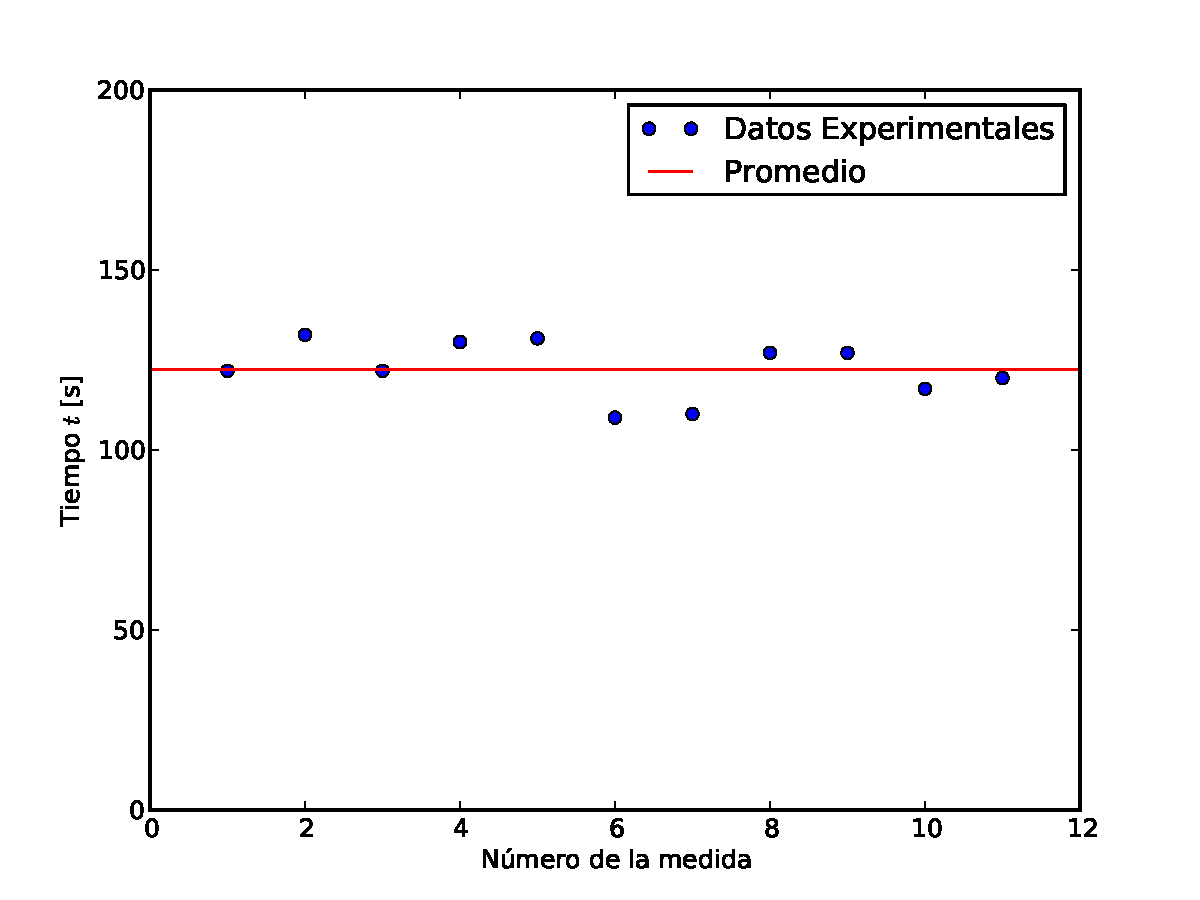
\includegraphics[width=10cm]{figs/fig-ajuste-promedio.pdf}
\caption{El ajuste por una constante es equivalente a calcular el promedio. C'odigo Python en ap'endice \ref{app-ajuste-promedio}.}
\end{center}
\end{figure}

*** Agregar ejemplo de \texttt{scipy.stats.linregress} ***

\section{Regresi'on Polinomial}

Algunos datos se representan pobremente mediante una l'inea recta. Para estos casos es mejor usar otro tipo de modelos. Por ejemplo, la llamada \textbf{regresi'on polinomial} se basa en ajustar el siguiente polinomio de grado $m$:
\begin{equation}
f(x) = a_0+a_1x+a_2x^2+\cdots + a_mx^m.
\end{equation}

En este caso
\begin{equation}\label{Srpol}
\chi^2 = \sum_{i=1}^N\left(y_i-f(x_i)\right)^2=\sum_{i=1}^N\left(y_i-a_0-a_1x_i-a_2x_i^2-\cdots - a_mx_i^m\right)^2,
\end{equation}

\begin{align}
\frac{\partial\chi^2}{\partial a_0} &= -2\sum_{i=1}^N \left(y_i-a_0-a_1x_i-a_2x_i^2-\cdots -a_mx_i^m\right) ,\\
\frac{\partial\chi^2}{\partial a_1} &= -2\sum_{i=1}^N x_i\left(y_i-a_0-a_1x_i-a_2x_i^2-\cdots -a_mx_i^m\right) ,\\
\vdots \quad &= \quad \vdots  \\
\frac{\partial\chi^2}{\partial a_p} &= -2\sum_{i=1}^N x_i^p\left(y_i-a_0-a_1x_i-a_2x_i^2-\cdots -a_mx_i^m\right) ,\\
\vdots \quad &= \quad \vdots  \\
\frac{\partial\chi^2}{\partial a_m} &= -2\sum_{i=1}^N x_i^m\left(y_i-a_0-a_1x_i-a_2x_i^2-\cdots -a_mx_i^m\right).
\end{align}
Igualando a cero y reordenando t'erminos, obtenemos
\begin{align}
a_0 N + a_1\sum_{i=1}^N x_i +a_2 \sum_{i=1}^N x_i^2 + \cdots + a_m \sum_{i=1}^N x_i^m &= \sum_{i=1}^N y_i, \\
a_0 \sum_{i=1}^N x_i + a_1\sum_{i=1}^N x_i^2 +a_2 \sum_{i=1}^N x_i^3 + \cdots + a_m \sum_{i=1}^N x_i^{m+1} &= \sum_{i=1}^N x_iy_i, \\
\vdots\quad &= \quad \vdots \\
a_0 \sum_{i=1}^N x_i^p + a_1\sum_{i=1}^N x_i^{p+1} +a_2 \sum_{i=1}^N x_i^{p+2} + \cdots + a_m \sum_{i=1}^N x_i^{p+m} &= \sum_{i=1}^N x_i^py_i, \\
\vdots\quad &= \quad \vdots \\
a_0 \sum_{i=1}^N x_i^m + a_1\sum_{i=1}^N x_i^{m+1} +a_2 \sum_{i=1}^N x_i^{m+2} + \cdots + a_m \sum_{i=1}^N x_i^{2m} &= \sum_{i=1}^N x_i^my_i.
\end{align}
Note que el n'umero de inc'ognitas ($a_0, a_1, a_2,\cdots a_m$) es igual al n'umero de ecuaciones ($m+1$). El sistema de ecuaciones anterior es lineal en las inc'ognitas, y puede escribirse en la forma est'andar como sigue:
\begin{equation}
\left(\begin{array}{cccccc}
N & \sum x_i & \cdots &  \sum x_i^k & \cdots & \sum x_i^m \\
\sum x_i &  \sum x_i^2 & \cdots &  \sum x_i^{k+1} & \cdots & \sum x_i^{m+1} \\
\vdots & \vdots & \cdots & \vdots & \ddots & \vdots \\
\sum x^p_i &  \sum x_i^{p+1} & \cdots &  \sum x_i^{p+k} & \cdots & \sum x_i^{p+m} \\
\vdots & \vdots & \cdots & \vdots & \ddots & \vdots \\
\sum x_i^m &  \sum x_i^{m+1} & \cdots &  \sum x_i^{k+m} & \cdots & \sum x_i^{2m} \\
\end{array}
\right)\left(\begin{array}{c}a_0\\a_1\\ \vdots\\a_p\\ \vdots\\a_m\end{array}\right)
=\left(\begin{array}{c}
\sum y_i\\ \sum x_iy_i\\ \vdots\\ \sum x_i^py_i\\ \vdots\\ \sum x_i^m y_i\end{array}\right).
\end{equation}

%El error en el ajuste polinomial se cuantifica mediante el \textbf{error est'andar} de la aproximaci'on,
%\begin{equation}
%S_{Y/x}=\sqrt{\frac{S_r}{N-(m+1)}},
%\end{equation}
%donde $m$ es el orden del polinomio. Esta cantidad se divide por $N-(m+1)$ ya que se usaron $m+1$ coeficientes. Adem'as del error est'andar podemos calcular el coeficiente de determinaci'on usando nuevamente la definici'on \eqref{r2} y \eqref{St}, pero donde ahora $S_r$ es dado por \eqref{Srpol}.

\paragraph{Ejemplo:}  Ajustar un polinomio de grado 2, para la siguiente tabla de valores \ref{tab-xt}.

\begin{table}[h!]
\begin{center}
\begin{tabular}{|c|c|}
\hline 
Posici'on & Tiempo \\ 
$x$, [m] $\pm 0,1$ & $t$, [s] $\pm 0,01$ \\ \hline
0.00 & 2.1 \\ \hline
1.00 & 7.7 \\ \hline
2.00 & 13.6\\ \hline
3.00 & 27.2\\ \hline
4.00 & 40.9\\ \hline
5.00 & 61.1\\ \hline
\end{tabular}
\caption{Posici'on de un movimiento unidimensional como funci'on del tiempo.}
\label{tab-xt}
\end{center}
\end{table}

%\subsection{Regresi'on lineal m'ultiple}
%
%Una extensi'on 'util de la regresi'on lineal es cuando $y$ es funci'on de dos o m'as variables:
%\begin{equation}
%y=f(x) = a_0 + a_1x_1+a_2x_2+\cdots + a_mx_m.
%\end{equation}
%An'alogamente a los casos anteriores, los ``mejores'' coeficientes quedan determinados minimizando el cuadrado de los residuos:
%\begin{equation}
%\chi^2=\sum_{i=1}^N\left(y_i-f(x_i)\right)^2=\sum_{i=1}^N\left(y_i-a_0-a_1x_1-a_2x_2-\cdots -a_mx_m\right)^2.
%\end{equation}
%En este caso las ecuaciones para los estimadores quedan determinadas por
%\begin{align}
%\frac{\partial\chi^2}{\partial a_0} &= -2\sum_{i=1}^N \left(y_i-a_0-a_1x_{1,i}-a_2x_{2,i}-\cdots -a_mx_{m,i}\right) ,\\
%\frac{\partial\chi^2}{\partial a_1} &= -2\sum_{i=1}^N x_{1,i}\left(y_i-a_0-a_1x_{1,i}-a_2x_{2,i}-\cdots -a_mx_{m,i}\right) ,\\
%\frac{\partial\chi^2}{\partial a_2} &= -2\sum_{i=1}^N x_{2,i}\left((y_i-a_0-a_1x_{1,i}-a_2x_{2,i}-\cdots -a_mx_{m,i}\right) ,\\
%\vdots\quad &= \quad\vdots \\
%\frac{\partial\chi^2}{\partial a_m} &= -2\sum_{i=1}^N x_{m,i}\left((y_i-a_0-a_1x_{1,i}-a_2x_{2,i}-\cdots -a_mx_{m,i}\right) .
%\end{align}
%Igualando a cero y reordenando t'erminos, obtenemos
%\begin{align}
%a_0 N + a_1\sum_{i=1}^N x_{1,i} +a_2 \sum_{i=1}^N x_{2,i}+\cdots+a_m \sum_{i=1}^N x_{m,i} &= \sum_{i=1}^N y_i, \\
%a_0 \sum_{i=1}^N x_{1,i} + a_1\sum_{i=1}^N x_{1,i}^2 +a_2 \sum_{i=1}^N x_{1,i}x_{2,i}+\cdots  +a_m \sum_{i=1}^N x_{1,i}x_{m,i}&= \sum_{i=1}^N x_{1,i}y_i, \\
%a_0 \sum_{i=1}^N x_{2,i} + a_1\sum_{i=1}^N x_{2,i}x_{1,i} +a_2 \sum_{i=1}^N x_{2,i}^2 + \cdots +a_m \sum_{i=1}^N x_{2,i}x_{m,i}&= \sum_{i=1}^N x_{2,i}y_i,\\
%\vdots\quad &= \quad\vdots \\
%a_0 \sum_{i=1}^N x_{m,i} + a_1\sum_{i=1}^N x_{m,i}x_{1,i} +a_2 \sum_{i=1}^N x_{m,i}x_{2,i} + \cdots +a_m \sum_{i=1}^N x_{m,i}^2&= \sum_{i=1}^N x_{m,i}y_i.
%\end{align}
%Esto define el siguiente sistema lineal de ecuaciones para ($a_0,a_1,a_2,\dots a_m$):
%\begin{equation}
%\left(\begin{array}{ccccc}
%N & \sum x_{1,i} & \sum x_{2,i} & \cdots &  \sum x_{m,i} \\
%\sum x_{1,i} & \sum x_{1,i}x_{1,i} & \sum x_{1,i}x_{2,i} &\cdots & \sum x_{1,i}x_{m,i}  \\
%\sum x_{2,i} & \sum x_{2,i}x_{1,i} & \sum x_{2,i}x_{2,i} &\cdots & \sum x_{2,i}x_{m,i}  \\
%\vdots & \vdots  & \vdots & \ddots & \vdots \\
%\sum x_{m,i} & \sum x_{m,i}x_{1,i} & \sum x_{m,i}x_{2,i} &\cdots & \sum x_{m,i}x_{m,i}  \\
%\end{array}\right)
%\left(\begin{array}{c} a_0\\a_1\\a_2\\ \vdots \\ a_m\end{array}\right)
%=
%\left(\begin{array}{c} \sum y_i\\\sum x_{1,i}y_i\\\sum x_{2,i}y_i \\\vdots\\ \sum x_{m,i}y_i\end{array}\right)
%\end{equation}
%
%\paragraph{Ejemplo:} Determine el ``mejor'' plano que ajusta los valores en la tabla \ref{tab-xyz} y eval'ue el error est'andar.
%\begin{table}[h!]
%\begin{center}
%\begin{tabular}{c|c|c}
%$x$ & $y$ & $z$ \\ \hline
%0 & 0 & 5 \\ 
%2 & 1 & 10 \\ 
%2.5 & 2 & 9 \\ 
%1 & 3 & 0 \\ 
%4 & 6 & 3 \\ 
%7 & 2 & 27 \\ 
%\end{tabular}
%\caption{Datos para la Tarea: valores de $x$, $y$ y $z$.}
%\label{tab-xyz}
%\end{center}
%\end{table}
%
%\begin{figure}[h!]
%\begin{center}
%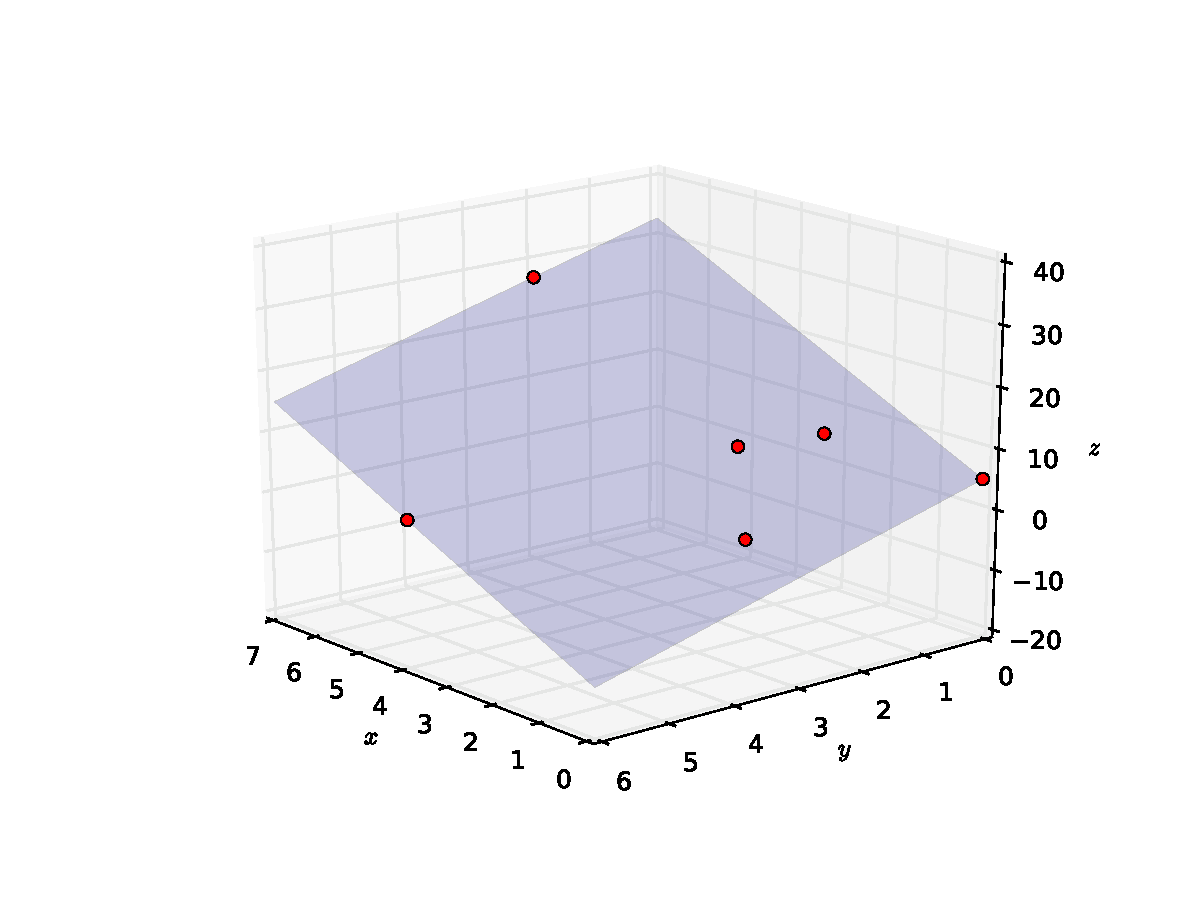
\includegraphics[width=10cm]{figs/fig-ajuste-plano.pdf}
%\caption{Ajuste por m'inimos cuadrados de los datos por un plano. C'odigo Python en ap'endice \ref{app-ajuste-plano}. En este caso ajustamos una funci'on $z=a_0+a_1x+a_2y$. Los coeficientes resultantes son $a_0=5.0$, $a_1=4.0$ y $a_2=-3.0$. El coeficiente de determinaci'on resulta ser $r^2=1$.}
%\end{center}
%\label{fig-ajuste-plano}
%\end{figure}
%

\section{M'etodo de M'inimos Cuadrados para una funci'on arbitraria}
Discutiremos ahora el caso en el que la funci'on que queremos ajuster (``el modelo'') no es un polinomio, sino una funci'on en principio arbitraria, $f(x)$, que dependa de algunos par'ametros a determinar.
%
%Supongamos que el modelo propuesto est'a dado por:
%\begin{equation}
%Y = f(x)+\epsilon,
%\end{equation}
%donde $\epsilon$  es un error aleatorio con $E(\epsilon)=0$ y  varianza $V(\epsilon)=\sigma^{2}$ constante. Tal como se mencion'o anteriormente, la idea de varianza constante consiste en que si el intervalo es dividido en sub-intervalos todos poseen la misma varianza. Esto mismo visto de manera intuitiva, consiste en que la dispersi'on de los datos (en $y$) respecto a la curva ajustada (modelo) debe ser (aproximadamente) independiente de $x$.
%
%\subsubsection{Ajuste de una funci'on arbitraria por m'inimos cuadrados}

Esto consiste en definir la siguiente funcional: 
\begin{equation}
\chi^2=\sum_{i=1}^N\left(y_i-f(x_i)\right)^2.
\end{equation}

Tal como en los casos anteriore, $\chi^2$ satisface:
\begin{enumerate}
\item $\chi^2$ es una magnitud definida como positiva, es decir $\chi^2\geq 0$.
\item $\chi^2 = 0$ si y s'olo si $y_i = f(x_i)$, $\forall i$, es decir, si la funci'on pasa exactamente por todos los puntos.
\end{enumerate}

%Adem'as, se exige que los residuos satisfagan $E(\epsilon)= 0$. El m'etodo de m'inimos cuadrados garantiza autom'aticamente que se satisface esta condici'on.

Normalmente no se cumple la condici'on $y_i = f(x_i)$, por lo que $\chi^2$ nunca es cero. La forma de determinar los par'ametros ajustables de la funci'on $f$ es hacer que $\chi^2$ sea lo m'as pr'oximo a cero, lo que se logra \textit{minimizando} su valor con respecto a los par'ametros ajustables. Al realizar esto, se obtiene una funci'on que describe, s'olo de manera aproximada, la tendencia general de los puntos experimentales.
Por lo tanto, el problema de encontrar $f$ se traduce en minimizar la funcional $\chi^2$ para una familia de funciones dada. 
%Note que solamente nos hemos concentrado en minimizar las distancias entre la variable dependiente del modelo con los datos experimentales $y_{i}$ y las variables independientes las hemos considerado fijas, es decir, no consideramos su incertidumbre.
\begin{figure}[h!]
\begin{center}
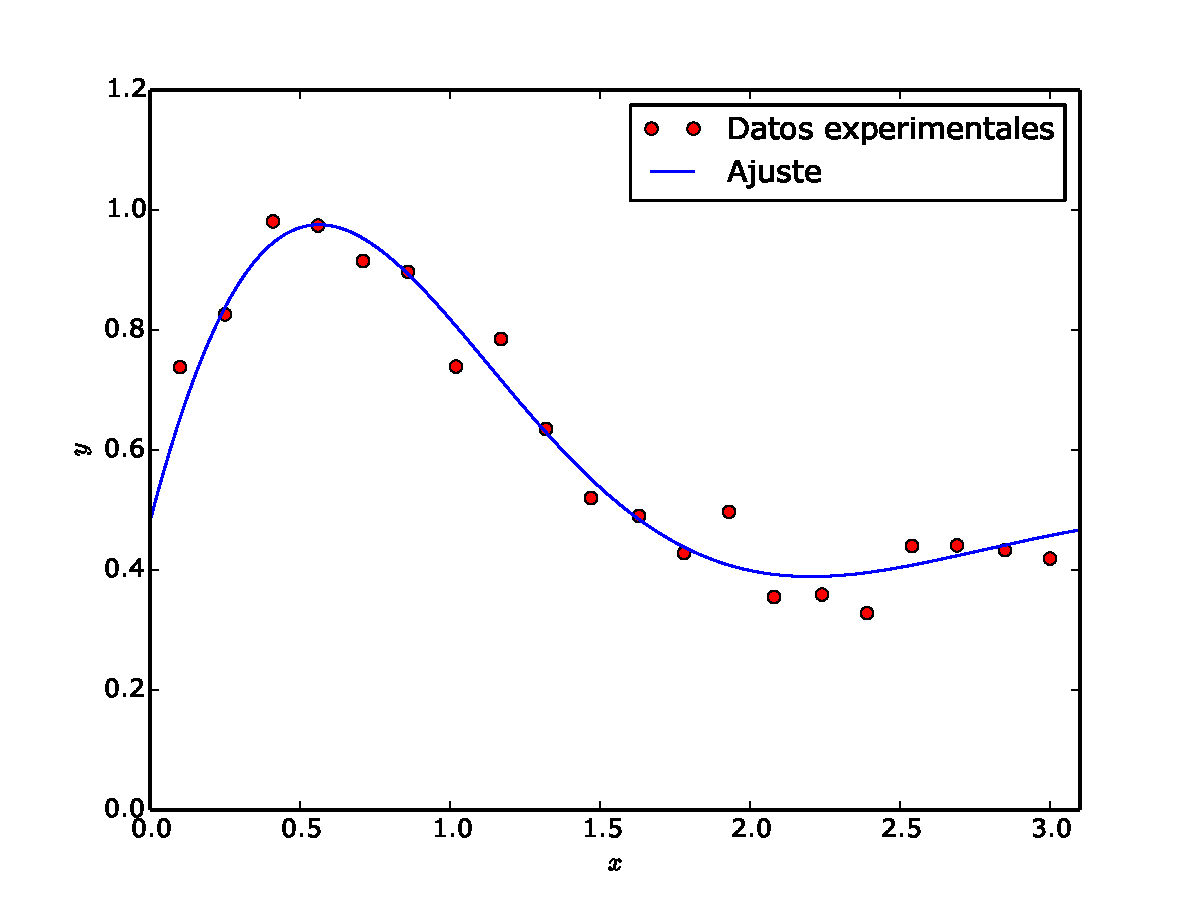
\includegraphics[width=10cm]{figs/fig-mmc-2.pdf}
\caption{Ajuste no-polinomial de datos usando el m'etodo de m'inimos cuadrados. C'odigo Python en ap'endice \ref{app-10}.}
\end{center}
\label{fig-mmc-2}
\end{figure}
\subsection{Implementaci'on en Python}
En Python existen varios m'odulos y funciones que implementan el MMC para una funci'on arbitraria. En general 'estos se basan en algoritmos ``de optimizaci'on" en los que se busca que alguna funci'on ``objetivo'' sea m'axima (o m'inima). En nuestro caso, se buscan los par'ametros de la funci'on $f(x)$ tales que el valor de $\chi^2$ sea el m'inimo (o, equivalentemente que $-\chi^2$ sea m'aximo). Varios m'etodos de optimizaci'on est'an implementados en el m'odulo \texttt{scipy.optimize} de Scipy, en particular la funci'on \texttt{scipy.optimize.minimize}. Sin embargo, para el caso particular de aplicaci'on de este tipo de m'etodos al problema del ajuste de curvas por medio del MMC, existen funciones espec'ificas m'as c'omodas de usar, tales como \texttt{scipy.optimize.least\_squares} o bien \texttt{scipy.optimize.curve\_fit} (que, de hecho, llama internamente a \texttt{scipy.optimize.least\_squares}).

\section{Método de m'inimos Cuadrados Ponderados}

Si el error o incerteza de los valores de $y_i$ no es constante podemos introducir una mejora para estimar los parámetros de ajuste por mínimos cuadrados, introduciendo la idea de \textbf{mínimos cuadrados ponderados}. Esta variación del método implementa la idea que no todos los valores $y_{i}$ son igualmente confiables, dado que el error asociado a cada uno de ellos, que denotaremos por $\sigma_i$ asume un valor distinto, dando un mayor peso a los datos con menor error y viceversa. En particular, a cada dato $y_i$ se le asocia un peso $p_{i}$, tal que ahora
\begin{equation}
\chi^2=\sum_{i=1}^N p_i\left(y_i-f(x_i)\right)^2.
\end{equation}

Luego repetimos el mismo procedimiento utilizado por el m'etodo de mínimos cuadrados ordinarios visto anteriormente, minimizando la función $\chi^2$. Esto conduce a nuevos valores de los parámetros de la función $f$ que hayamos elegido como modelo. 

\subsubsection{Ajuste de un modelo lineal}
En el caso de ajustar una recta, podemos obtener rápidamente las expresiones para la nueva pendiente y coeficiente de posición reemplazando en cada una de las expresiones encontradas en el caso del MMC ordinario las sumas $\sum_{i=1}^N$ por $\sum_{i=1}^Np_{i}$:
\begin{equation}\label{b0MMCP}
b_0 = \frac{\left(\sum_{i=1}^N p_{i}y_{i}\right)\left(\sum_{i=1}^N p_{i}x_{i}^2\right)-\left(\sum_{i=1}^N p_{i}x_{i} y_{i}\right)\left(\sum_{i=1}^N p_{i}x_{i}\right)}
{\left(\sum_{i=1}^N p_{i}\right)\left(\sum_{i=1}^N p_{i}x_{i}^{2}\right)-\left(\sum_{i=1}^N p_{i}x_{i}\right)^{2}},
\end{equation}
\begin{equation}\label{b1MMCP}
b_1 =  \frac{\left(\sum_{i=1}^N p_{i}\right)\left(\sum_{i=1}^N p_{i}x_{i} y_{i}\right)-\left(\sum_{i=1}^N p_{i}x_{i}\right)\left(\sum_{i=1}^N p_{i}y_{i}\right)}
{\left(\sum_{i=1}^N p_{i}\right)\left(\sum_{i=1}^N p_{i}x_{i}^{2}\right)-\left(\sum_{i=1}^N p_{i}x_{i}\right)^{2}}. 
\end{equation}

\subsubsection{Ajuste polinomial}

\begin{equation}
\left(\begin{array}{ccccc}
\sum p_i & \sum p_ix_i &  \sum p_ix_i^2 & \cdots & \sum p_ix_i^m \\
\sum p_ix_i &  \sum p_ix_i^2 &  \sum p_ix_i^3 & \cdots & \sum p_ix_i^{m+1} \\
\sum p_ix^2_i &  \sum p_ix_i^3 &  \sum p_ix_i^4 & \cdots & \sum p_ix_i^{m+2} \\
\vdots & \vdots & \vdots & \ddots & \vdots \\
\sum p_ix_i^m &  \sum p_ix_i^{m+1}&  \sum p_ix_i^{m+2} & \cdots & \sum p_ix_i^{2m}
\end{array}
\right)\left(\begin{array}{c}a_0\\a_1\\a_2\\ \vdots\\a_m\end{array}\right)
=\left(\begin{array}{c}
\sum p_iy_i\\ \sum p_ix_iy_i\\ \sum p_ix_i^2y_i\\ \vdots\\ \sum p_ix_i^m y_i\end{array}\right).
\end{equation}

%\subsubsection{Ajuste lineal multiple}
%\begin{equation}
%\left(\begin{array}{ccccc}
%\sum p_i & \sum p_ix_{1,i} & \sum p_ix_{2,i} & \cdots &  \sum p_ix_{m,i} \\
%\sum p_ix_{1,i} & \sum p_ix_{1,i}x_{1,i} & \sum p_ix_{1,i}x_{2,i} &\cdots & \sum p_ix_{1,i}x_{m,i}  \\
%\sum p_ix_{2,i} & \sum p_ix_{2,i}x_{1,i} & \sum p_ix_{2,i}x_{2,i} &\cdots & \sum p_ix_{2,i}x_{m,i}  \\
%\vdots & \vdots  & \vdots & \ddots & \vdots \\
%\sum p_ix_{m,i} & \sum p_ix_{m,i}x_{1,i} & \sum p_ix_{m,i}x_{2,i} &\cdots & \sum p_ix_{m,i}x_{m,i} 
%\end{array}\right)
%\left(\begin{array}{c} a_0\\a_1\\a_2\\ \vdots \\ a_m\end{array}\right)
%=
%\left(\begin{array}{c} \sum p_iy_i\\\sum p_ix_{1,i}y_i\\\sum p_ix_{2,i}y_i \\\vdots\\ \sum x_{m,i}y_i\end{array}\right).
%\end{equation}

Notemos que no hemos dado una forma expl'icita para los pesos $p_i$ y eso se debe a que no hay una 'unica manera de definirlos. Por ejemplo, un buen criterio podr'ia ser que los pesos sean inversamente proporcionales a la incertidumbre, es decir, le dar'iamos mayor credibilidad a los $y_{i}$ con menos incertidumbre y menor credibilidad a los $y_{i}$ con mayor incertidumbre. Para esto es com'un elegir $p_i=1/(\Delta y_{i})^2$. Una conveniente consecuencia adicional de esta elección es que la función $\chi^2$ será siempre \textit{adimensional}.

\paragraph{Ejemplo:} Considere los datos de la siguiente tabla:
\begin{table}[h!]
\begin{center}
\begin{tabular}{c|c}
$x$ & $y\pm\Delta y$ \\ \hline
$1.0$ & $2.8\pm 0.3$ \\ \hline 
$2.0$ & $3.3\pm 0.3$ \\ \hline
$3.0$ & $3.5\pm 0.5$ \\ \hline
$4.0$ & $3.5\pm 1.0$ \\ \hline
$5.0$ & $4.8\pm 0.3$\\ \hline
$6.0$ & $4.2\pm 1.0$ 
\end{tabular}
\caption{Valores de $x$ e $y$, con error en $y$.}
\label{tab-xyDy}
\end{center}
\end{table}
Podemos comparar el resultado de ajustar una recta a estos datos usando el m'etodo de m'inimos cuadrados tradicional (sin ponderar, es decir, sin tomar en cuenta los valores de $\Delta y$) y el m'etodo de m'inimos cuadrados ponderado (eligiendo $p_i=1/(\Delta y_{i})^2$).
\begin{figure}[h!]
\begin{center}
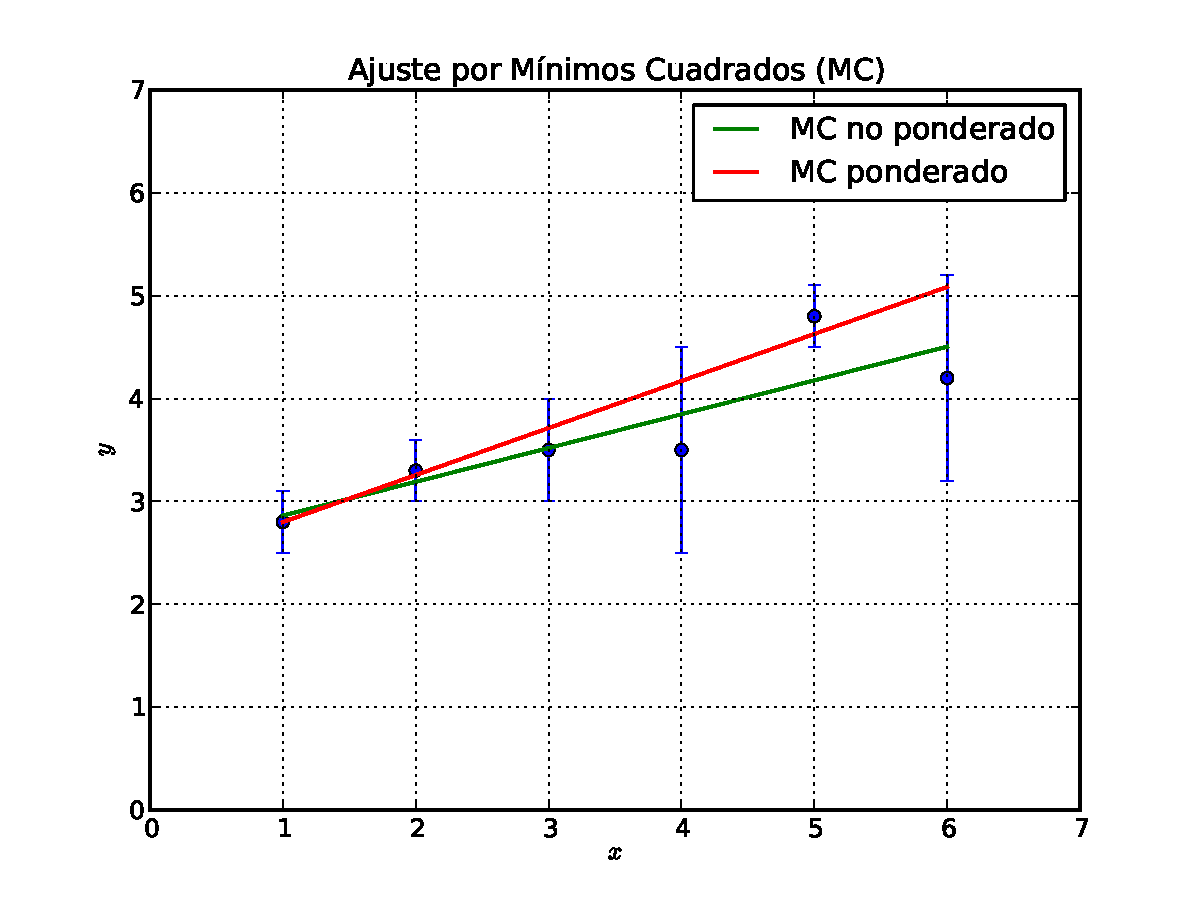
\includegraphics[width=10cm]{figs/fig-mc-ponderado.pdf}
\caption{Ajuste por m'inimos cuadrados con y sin poderaci'on.}
\end{center}
\end{figure}

%\subsection{m'axima Verosimilitud}
%
%Otro m'etodo para estimar los par'ametros de los modelos es maximizando la \textbf{funci'on de verosimilitud}.
%
%Supongamos que disponemos del siguiente modelo a ser ajustado,
%\begin{equation}
%Y=f(x)+\epsilon,
%\end{equation}
%y que \textit{conocemos las distribuci'on de los residuos} $g(\epsilon)$. En este caso podr'iamos construir la funci'on verosimilitud, definida por
%\begin{equation}
%L(b_{0},b_{1},\dots, \sigma^{2})=\prod_{i=1}^{N} g(y_{i}- f(x_{i})).
%\end{equation}
%\textit{Maximizando} la funci'on verosimilitud (o, equivalentemente, su logaritmo) con respecto a los $N+1$ par'ametros ajustables o estimadores de los par'ametros del modelo propuesto, encontramos
%\begin{align}
%\frac{\partial\ln L(b_{0,}\dots,b_{i,}\dots b_{N},\sigma^{2})}{\partial b_{0}} &=0,\\ 
%\vdots\qquad &= 0,\\
%\frac{\partial\ln L(b_{0,}\dots,b_{i,}\dots b_{N},\sigma^{2})}{\partial b_{i}}&=0, \\
%\vdots\qquad &= 0,\\  
%\frac{\partial\ln L(b_{0,}\dots,b_{i,}\dots b_{N},\sigma^{2})}{\partial b_{N}}&=0.
%\end{align}
%Agregamos otra condici'on que nos permite determinar el valor de la varianza:
%\begin{equation}
%\frac{\partial\ln L(b_{0}\dots,b_{i,}\dots b_{N},\sigma^{2})}{\partial \sigma^{2}}=0.
%\end{equation}
%
%Resolviendo este conjunto de $N+2$ ecuaciones, quedan determinados los estimadores de los coeficientes y la varianza.
%
%Note que si la distribuci'on de los residuos es normal, el m'etodo de m'axima verosimilitud entrega los mismos valores para los par'ametros $b_{1},b_{1},\dots b_{N}$ que m'inimos cuadrados.
%
%\paragraph{Ejemplo:} Supongamos que deseamos ajustar un modelo lineal y sabemos que los residuos tienen una distribucion normal 
%\\
%\begin{equation}
%f(\epsilon,\sigma) = \frac{1}{\sqrt{2\pi\sigma^2}} e^{-\frac{1}{2}\left(\frac{\epsilon}{\sigma}\right)^2}.
%\end{equation}
%
%Modelo: $ Y=\beta_{0}+\beta_{1}x+\epsilon$ y para los datos de la muestra de tama\~no $N$ se cumple que $y_{i}=\beta_{0}+\beta_{1}x_{i}+\epsilon_{i}$ con $i=1,\dots,N$.
%
%En este caso, la funci'on verosimilitud queda definida como
%\begin{equation}
%L(b_{0},b_{1},\sigma^{2})=\prod_{i=1}^{N} f(y_{i}- b_{0}-b_{1}x_{i}) =\prod_{i=1}^{N} \frac{1}{\sqrt{2\pi\sigma^2}} e^{-\frac{1}{2}\left(\frac{y_{i}-b_{0}-b_{1}x_{i}}{\sigma}\right)^2}.
%\end{equation}
%
%Maximizando $\ln L(b_{0},b_{1},\sigma^{2})$ respecto de los par'ametros $b_{0}, b_{1}$ y $\sigma^2$ se obtienen tres ecuaciones,
%\begin{align}
%\frac{\partial \ln  L(b_{0},b_{1},\sigma^{2})}{\partial b_{0}} &= 0,\\
%\frac{\partial \ln  L(b_{0},b_{1},\sigma^{2})}{\partial b_{1}} &=0,\\
%\frac{\partial \ln  L(b_{0},b_{1},\sigma^{2})}{\partial \sigma^2} &=0,
%\end{align}
%donde las dos primeras ecuaciones nos conducen a las mismas soluciones de ambos estimadores $b_{0}$ y $b_{1}$, para el caso de distribuci'on normal de los residuos, que el metodo de m'inimos cuadrados. 

\section{an'alisis (Gr'afico e histograma) de residuos}

%\begin{figure}[h!]
%\begin{center}
%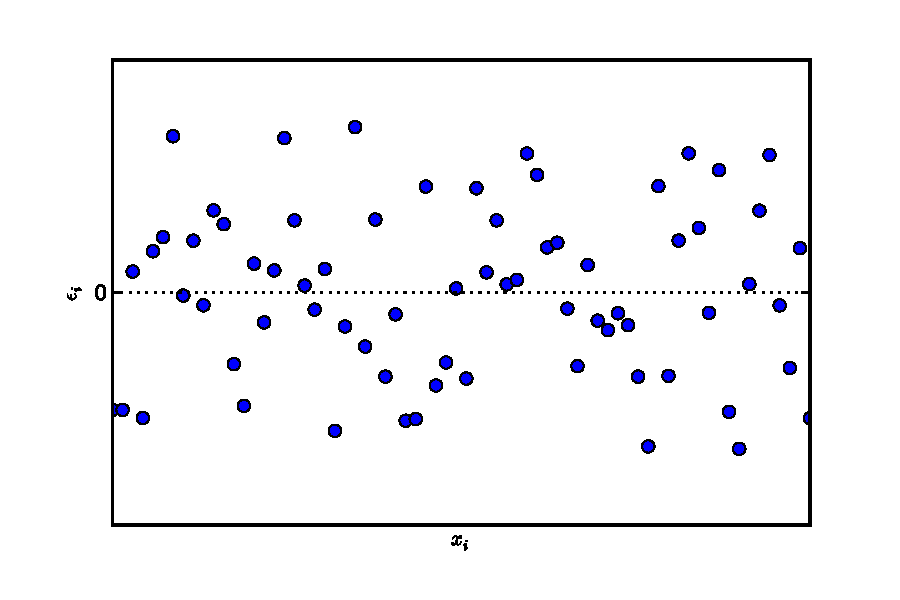
\includegraphics[width=7cm]{figs/fig-dispersion-01.pdf}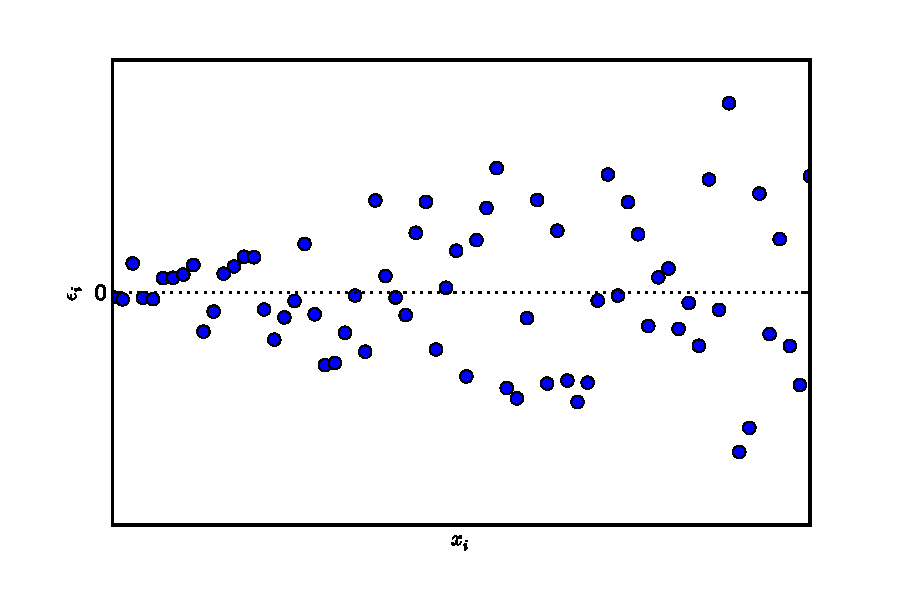
\includegraphics[width=7cm]{figs/fig-dispersion-02.pdf}\\
%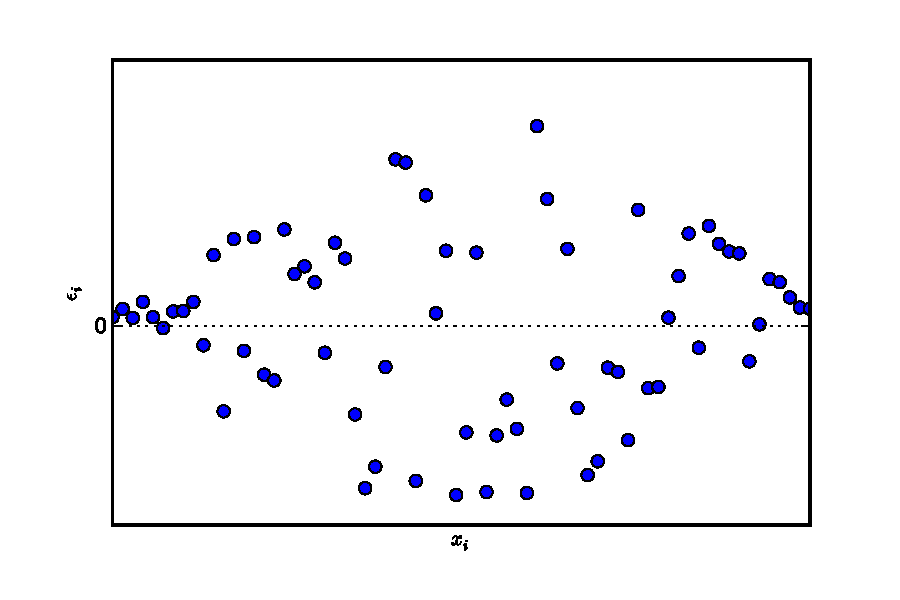
\includegraphics[width=7cm]{figs/fig-dispersion-03.pdf}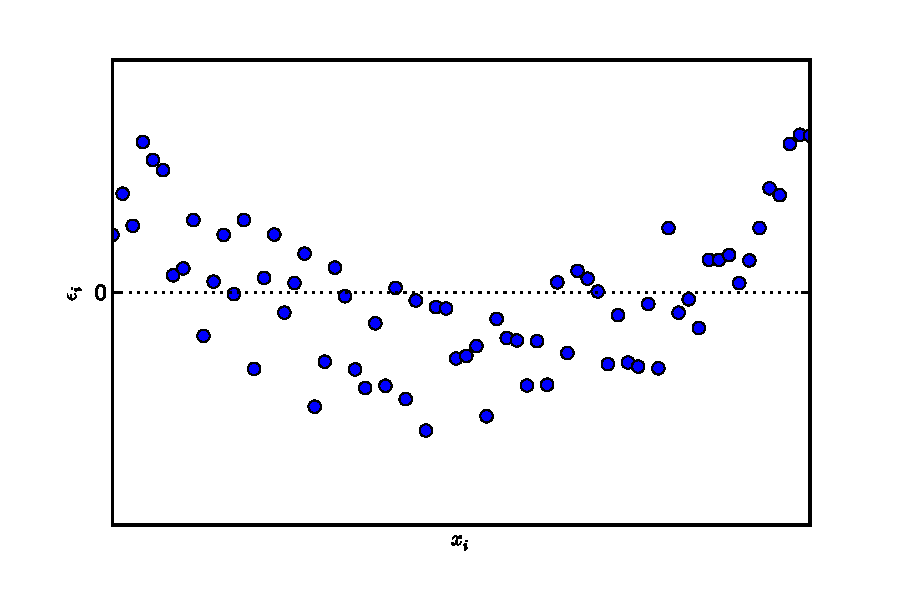
\includegraphics[width=7cm]{figs/fig-dispersion-04.pdf}
%\caption{Ejemplos de distintas posibilidades para la dispersi'on.}
%\end{center}
%\label{fig-disp}
%\end{figure}

%
%\section{Interpolaci'on}
%Con frecuencia es necesario estimar valores intermedios entre valores conocidos y de baja incerteza. El m'etodo m'as com'un que se emplea para este caso, es la \textbf{interpolaci'on polinomial}.
%
%Polinomios de interpolaci'on con diferencias divididas de Newton
%\subsection{Polinomios de interpolaci'on con diferencias divididas de Newton}
%\subsection{Interpolaci'on lineal}
%
%\begin{equation}
%\frac{f_1(x)-f(x_0)}{x-x_0}=\frac{f(x_1)-f(x_0)}{x_1-x_0} \quad\Rightarrow\quad 
%f_1(x)=f(x_0)+\frac{f(x_1)-f(x_0)}{x_1-x_0}(x-x_0)
%\end{equation}
%
%\begin{figure}[h!]
%\begin{center}
%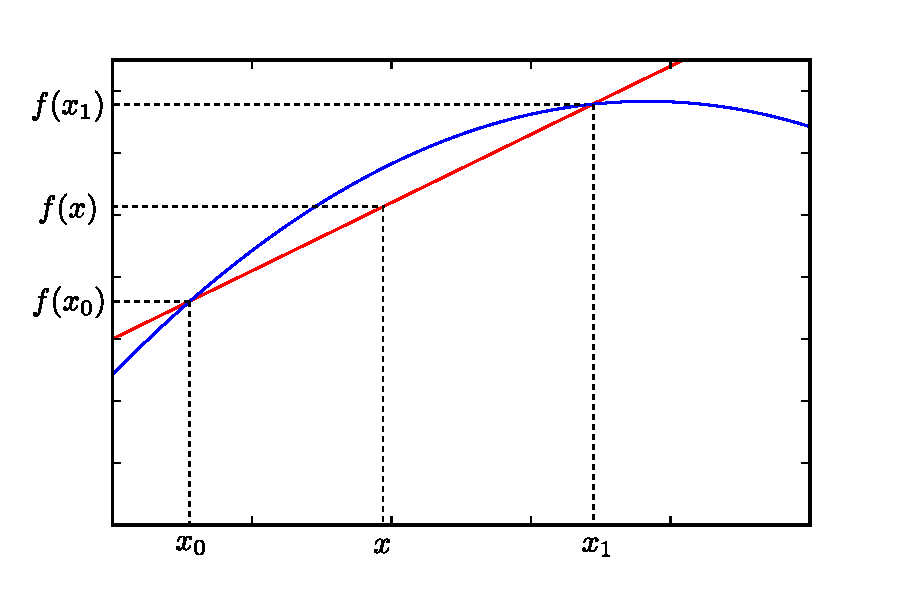
\includegraphics[width=10cm]{figs/fig-int-lineal-2.pdf}
%\caption{Interpolaci'on lineal.}
%\end{center}
%\end{figure}
%
%
%\subsection{Interpolaci'on cuadr'atica}
%
%\begin{equation}
%f_2(x)=b_0+b_1(x-x_0)+b_2(x-x_0)(x-x_1),
%\end{equation}
%con 
%\begin{align}
%b_0 &= f(x_0), \\
%b_1 &= \frac{f(x_1)-f(x_0)}{x_1-x_0}, \\
%b_2 &= \frac{\frac{f(x_2)-f(x_1)}{x_2-x_1}-\frac{f(x_1)-f(x_0)}{x_1-x_0}}{x_2-x_0}.
%\end{align}
%Desarrollando y agrupando t'erminos,
%\begin{equation}
%f_2(x)=a_0+a_1x+a_2x^2,
%\end{equation}
%donde 
%\begin{align}
%a_0 &= b_0-b_1x_0+b_2x_0x_1, \\
%a_1 &= b_1-b_2x_0-b_2x_1, \\
%a_2 &= b_2.
%\end{align}
%
%\subsection{Forma general de los polinomios de interpolaci'on de Newton}
%\begin{equation}
%f_n(x)=b_0+b_1(x-x_0)+\cdots +b_n(x-x_0)(x-x_1)\cdots (x-x_{n-1}).
%\end{equation}
%Se requieren $n+1$ puntos para obtener un polinomio de grado en'esimo o en'esimo orden.
%\begin{align}
%b_0 &= f(x_0), \\
%b_1 &= f[x_1,x_0], \\
%b_2 &= f[x_2,x_1,x_0], \\
% & \vdots \\
%b_n &= f[x_n,x_{n-1},\cdots, x_2,x_1,x_0],
%\end{align}
%
%\begin{align}
%f[x_i,x_j] &= \frac{f(x_i)-f(x_j)}{x_i-x_j}, \\
%f[x_i,x_j,x_k] &= \frac{f[x_i,x_j]-f[x_j,x_k]}{x_i-x_k}, \\
%& \vdots\\
%f[x_n,x_{n-1},\cdots,x_1,x_0] &= \frac{f[x_n,x_{n-1},\cdots, x_1]-f[x_{n-1},x_{n-2},\cdots,x_1,x_0]}{x_n-x_0}.
%\end{align}
%
%\subsection{Polinomios de interpolaci'on de Lagrange}
%
%Este polinomio de interpolaci'on, es una reformulaci'on del polinomio de Newton que evita los c'alculos de las diferencias divididas. Estos se representan como:
%\begin{equation}
%f_n(x)=\sum_{i=0}^nL_i(x)f(x_i),
%\end{equation}
%donde
%\begin{equation}
%L(x)=\prod_{{i=0}\atop{j\neq i}}^n\frac{x-x_j}{x_i-x_j}
%\end{equation}
%
%\subsection{Interpolaci'on lineal}
%\begin{equation}
%f_1(x)=\frac{x-x_1}{x_0-x_1}f(x_0)+\frac{x-x_0}{x_1-x_0}f(x_1).
%\end{equation}
%
%\subsection{Interpolaci'on cuadr'atica}
%\begin{equation}
%f_2(x)=\frac{(x-x_1)(x-x_2)}{(x_0-x_1)(x_0-x_2)}f(x_0)+\frac{(x-x_0)(x-x_2)}{(x_1-x_0)(x_1-x_2)}f(x_1)+\frac{(x-x_0)(x-x_1)}{(x_2-x_0)(x_2-x_1)}f(x_2)
%\end{equation}


%\chapter{Estimadores y m'etodo de m'axima Verosimilitud}
%
%
%Uno de los mejores m'etodos para obtener un estimador puntual de un par'ametro es el \textbf{m'etodo de m'axima verosimilitud} y como lo dice su nombre, el estimador ser'a el valor del par'ametro que m'aximiza la \textbf{funci'on de verosimilitud}, es decir, el valor que haga m'axima la probabilidad de obtener la muestra observada.
%Para poder comprender este m'etodo comenzaremos por definir algunos conceptos.
%
%\paragraph{Definici'on:} \textbf{estad'istica o estad'igrafos} es cualquier funci'on de las observaciones contenidas en una muestra aleatoria (promedio, varianza, etc).
%
%\paragraph{Definici'on:} \textbf{Estimaci'on puntual} es una estimaci'on n'umerica de la estad'istica que se desee evaluar. Por ejemplo, el estimador de $\mu$ (promedio de la poblaci'on) de una muestra aleatoria es $\bar{x}$ (promedio de la muestra).
%
%\section{Promedio, mediana, desviaci'on est'andar, varianza}
%
%
%\section{Definici'on de m'axima verosimilitud.}
%Sup'onga que $X$ es una variable aleatoria con distribuci'on de probabilidad $f(x,\theta)$, donde $\theta$ es un par'ametro desconocido. Sean $x_1,x_2,\dots, x_N$ los valores observados en una muestra aleatoria de tama\~no $N$. La \textbf{funci'on de verosimilitud} de la muestra es
%\begin{equation}
%L(\theta):=f(x_1 ,\theta)f(x_2,\theta)\cdots f(x_N ,\theta)
%\end{equation} 
%
%Note que la funci'on de verosimilitud es ahora una funci'on del par'ametro desconocido $\theta$. El \textbf{estimador de m'axima verosimilitud} de $\theta$ es el valor de $\theta$ que \textit{maximiza} la funci'on de verosimilitud $L(\theta)$.
%
%Note que para el caso de una variable aleatoria discreta, la interpretaci'on de la funci'on de verosimilitud $L(\theta)$ es la probabilidad
%\begin{equation}
%L(\theta)=P(X_1=x_1, X_2=x_2,\dots, X_N=x_N),
%\end{equation} 
%es decir, la probabilidad de obtener los valores Muestrales $x_1,\dots,x_N$. Para que esta 'ultima afirmaci'on sea v'alida, las probabilidades representadas por cada miembro del producto deben ser independientes.
%As'i, el estimador de m'axima verosimilitud es un estimador que maximiza la probabilidad de ocurrencia de los valores muestrales.
%
%\paragraph{Ejemplo:} Sea $X$ una variable aleatoria con \textit{distribuci'on normal}, con media desconocida y varianza conocida. La funci'on verosimilitud de una muestra de tama\~no $N$ es
%\begin{align}\label{Lmusigma}
%L(\mu,\sigma)&= \prod_{i=1} ^N \frac{1}{\sqrt{2\pi\sigma^2}}e^{-\frac{1}{2}\left(\frac{x-\mu}{\sigma}\right)^2} \\
%&= \frac{1}{(2\pi\sigma^2)^\frac{N}{2}}\exp\left[{-\frac{1}{2 \sigma^2 }\Sigma_{i=1} ^N ({x_i-\mu})^2}\right].
%\end{align}
%Calculando el logaritmo natural de ambos lados, encontramos
%\begin{equation}\label{lnL}
%\ln L(\mu)=-\frac{N}{2}\ln\left(2\pi\sigma^2\right)-(2\sigma^1)^{-1}\sum_{i=1}^N(x_i-\mu)^2.
%\end{equation}
%Derivando respecto al par'ametro desconocido $\mu$ e igualando a cero, llegamos a
%\begin{equation}
%\frac{d\ln L(\mu)}{d\mu}=(\sigma^2)^{-1} \sum_{i=1}^N(x_i-\mu)\stackrel{!}{=}0,
%\end{equation}
%que tiene como soluci'on para $\mu$ a
%\begin{equation}
%\hat{\mu}=\frac{1}{N}\sum_{i=1}^Nx_i=\bar{x},
%\end{equation}
%es decir, un estimador de la media $\mu$ es el valor de la media muestral.
%
%
%
%
%\paragraph{Ejemplo:} Sea $X$ una variable aleatoria con distribuci'on normal, donde tanto la media como la varianza son desconocidas. Ya sabemos que la funci'on verosimilitud est'a dada por \eqref{Lmusigma}. Calculando ahora las derivadas parciales de \eqref{lnL} respecto a $\mu$ y $\sigma^2$, e igual'andolas a cero, encontramos
%\begin{equation}
%\frac{\partial\ln L(\mu,\sigma)}{\partial\mu}=(\sigma^2)^{-1}\sum_{i=1}^N(x_i-\mu)\stackrel{!}{=}0,
%\end{equation}
%\begin{equation}
%\frac{\partial\ln L(\mu,\sigma)}{\partial\sigma^2}=-\frac{N}{2\sigma^2}+\frac{1}{2\sigma^4}\sum_{i=1}^N(x_i-\mu)^2\stackrel{!}{=}0,
%\end{equation}
%que tiene por soluciones a
%\begin{equation}
%\hat{\mu}=\frac{1}{N}\sum_{i=1}^Nx_i=\bar{x}, \qquad \hat{\sigma}^2=\frac{1}{N}\sum_{i=1}^N(x_i-\mu)^2.
%\end{equation}
%
%*** Ojo que 'este no es exactamente $\sigma$, porque est'a dividido por $N$ !, lo cual quiere decir que el m'etodo de M'axima verosimilitud no garantiza obtener estimadores insesgados.***


%\chapter{Noci'on de Probabilidades}

\section{Introducci'on}

Al intentar repetir una misma medici'on, los resultados obtenidos no son exactamente iguales debido a peque\~nas variaciones en las variables que no est'an totalmente controladas. Otra posible fuente de error, podr'ia ser el instrumento de medici'on, ya que 'este puede sufrir peque\~nas variaciones para una misma medici'on. En consecuencia, se dice que dicho experimento tiene una \textbf{componente aleatoria}.	
	
	En algunos casos, las variaciones son tan peque\~nas que podr'ian ignorarse. Sin embargo, en general la componente aleatoria s'i est'a presente y su magnitud puede ser muy importante para obtener alguna conclusi'on. Por lo tanto, lo que buscamos es describir, cuantificar y modelar este tipo de variaciones.

En la figura \ref{fig-sistema-modelo} se muestra el esquema idealizado de un experimento, donde el resultado de un experimento depende s'olo del sistema f'isico bajo estudio y de los par'ametros iniciales del experimento.
\begin{figure}[h!]
\begin{center}
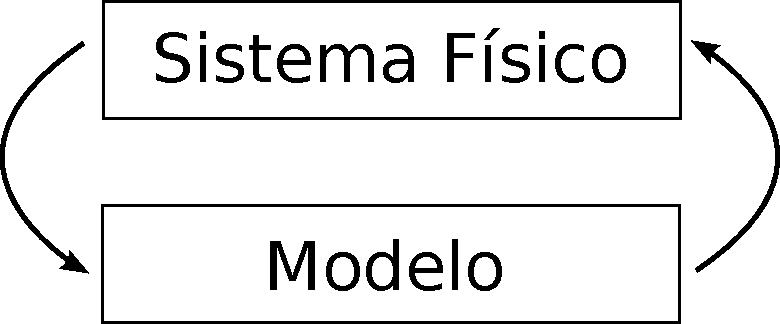
\includegraphics[width=6cm]{figs/fig-sistema-modelo.pdf}
\caption{Sistema f'isico y modelo.}
\end{center}
\label{fig-sistema-modelo}
\end{figure}
 Sin embargo, en la pr'actica siempre existen variables no controladas que pueden influir en el resultado (y/o puede ocurrir que el sistema bajo estudio presente propiedades intrinsecamente aleatorias, como ocurre con distintos sistemas con propiedades cu'anticas), por lo que un esquema un poco m'as realista ser'ia el que se muestra en la figura \ref{fig-entrada-sistema-salida-variables}.
\begin{figure}[h!]
\begin{center}

\includegraphics[width=10cm]{figs/fig-entrada-sistema-salida.pdf}
\caption{Entrada, sistema y salida.}
\end{center}
\label{fig-entrada-sistema-salida}
\end{figure}	
\begin{figure}[h!]
\begin{center}
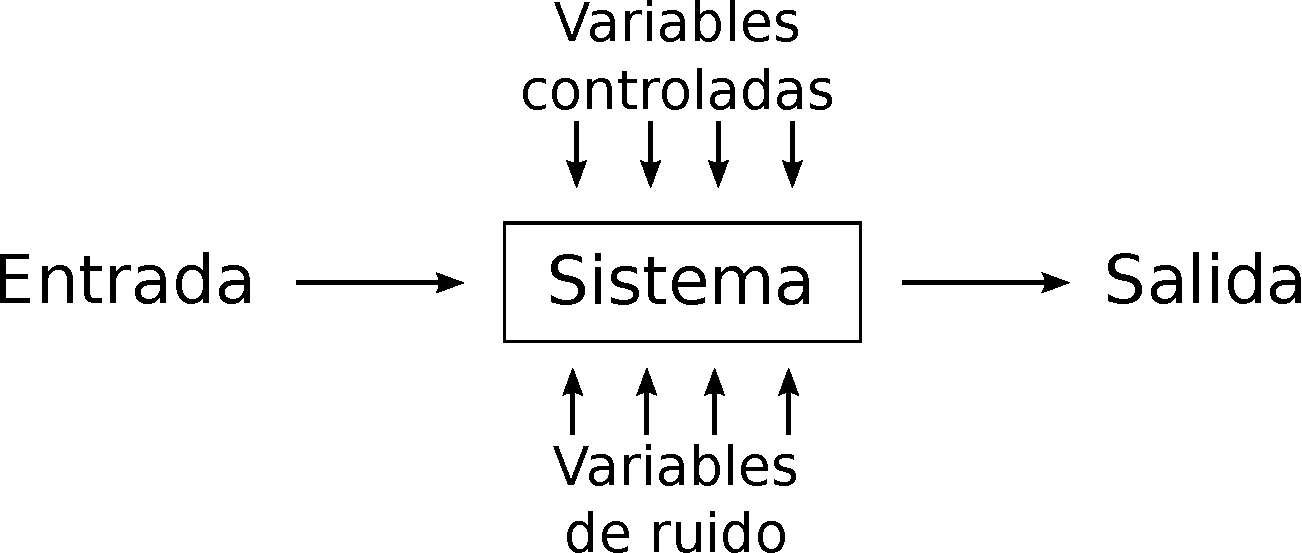
\includegraphics[width=10cm]{figs/fig-entrada-sistema-salida-variables.pdf}
\caption{Entrada, sistema, salida y variables.}
\end{center}
\label{fig-entrada-sistema-salida-variables}
\end{figure}

A continuaci'on introduciremos algunos conceptos b'asicos que resultan 'utiles en la definici'on y discusi'on de probabilidades.
		
\subsection{Experimento aleatorio}

Un \textbf{experimento aleatorio} es aquel que proporciona diferentes resultados a'un cuando se repita siempre de la ``misma manera''. Esto puedo ocurrir ya sea porque existen variables no  controladas o desconocidas que influyen y modifican el resultado, o bien porque el fen'omeno estudiado es intr'insicamente aleatorio.

\subsection{Poblaci'on}
La \textbf{poblaci'on} es un conjunto de elementos (individuos, objetos, etc.) con alguna caracter'istica com'un observable. A los elementos que conforman la poblaci'on se les llama \textbf{unidad observable} o \textbf{unidad de observaci'on}. Cuando se posee informaci'on de todas las unidades observables de la poblaci'on se est'a en presencia de un \textbf{censo}.

%\subsection{Muestra}
%Parte o porci'on extra'ida de una poblaci'on por m'etodos que permitan considerarla como representativa de la misma.


\subsection{Espacio muestral}

El conjunto de los posibles resultados de un experimento aleatorio recibe el nombre de \textbf{espacio muestral} del experimento. El espacio muestral se denotar'a con la letra $S$. Un espacio muestral es \textbf{discreto} si est'a formado por un conjunto de resultados contables.

\subsection{Evento}
Un evento es un subconjunto de un espacio muestral de un experimento aleatorio.
Dos eventos, $E_1$ y $E_2$, tales que $E_1\cap E_2=\emptyset$, se dice que son \textbf{mutuamente excluyentes}. Decimos que $X_i$ ($i=1,2,\cdots$) son \textbf{eventos elementales} si son mutuamente excluyentes ($X_i\cap X_j=\emptyset$, para $i\neq j$) y adem'as $\cup_i X_i=S$. En otras palabras, los eventos $X_i$ son tales que la ocurrencia de uno implica que ninguno de los otros eventos ocurre, y que cualquier otro evento no-elemental puede entenderse como la ocurrencia simult'anea de ellos.

\paragraph{Ejemplo 1:} Considere un experimento en el cual se miden dos variables y 'estas pueden tomar dos valores, $a$ o $b$. Los posibles resultados de dicho experimento ser'an:                                       $S=\{aa,ab,ba,bb\}$ y posibles eventos ser'an $E_1=\{aa\}$, $E_2=\{ab,ba\}$, $E_3=\{aa,ab,ba\}$, $E_4=\{ab,ba,bb\}$, $E_5=\{bb\}$.
		 
\paragraph{Ejemplo 2:} Supongamos que tenemos tres objetos $(1, 2, 3)$ y sacamos un par de 'estos. Todos los posibles resultados ser'an:
\begin{align}
S_1 &= \{12,13,21,23,31,32\}, \\
S_2 &= \{11,12,13,21,22,23,31,32,33\},
\end{align}
dependiendo si una vez sacado cada objeto, 'este es o no remplazado.
		 
\section{Interpretaci'on de la Probabilidad}

Es 'util cuantificar la posibilidad que se presente un resultado de un experimento aleatorio. La posibilidad de un resultado se cuantifica asign'andole un n'umero real en el intervalo $[0,1]$ o un porcentaje entre $0$ y $100\%$. Mientras m'as grande sea el n'umero, mayor ser'a la probabilidad de obtener ese resultado.

Una posible interpretaci'on de la probabilidad\footnote{Esta es la \textbf{interpretaci'on frecuentista}. En F'isica tambi'en es usada la \textbf{interpretaci'on Bayesiana}, que no discutiremos en mayor detalle en este curso.} se basa en el modelo de la \textit{repetici'on del experimento aleatorio}.
Sea $n(E)$ el n'umero de veces que ocurre el evento $E$ y $N$ el n'umero de veces que se realiza el experimento. Es intuitivamente razonable tomar como valor de $P(E)$ a
\begin{equation}
P(E):=\lim_{N\to\infty}f(E)=\lim_{N\to\infty}\frac{n(E)}{N},
\end{equation}
es decir, como el valor l'imite de la fracci'on de veces que el resultado $E$ aparece en $N$ repeticiones del experimento aleatorio, a medida que $N$ crece sin cota alguna. 

Por ejemplo, cada vez que un espacio muestral est'a formado por $d$ posibles resultados \textit{igualmente probables}, la probabilidad de cada uno de ellos ser'a $1/d$.

%Para un espacio muestral discreto, la probabilidad de un evento $E$, denotada como $P(E)$, es igual a la suma de las probabilidades de los resultados en $E$.
		
\section{Axiomas de probabilidad}

La probabilidad es un n'umero que se asigna a cada miembro de una colecci'on de eventos de un experimento aleatorio y que satisface las siguientes propiedades.

\begin{itemize}
\item Si $S$ es el espacio muestral y $E$ es cualquier evento del experimento aleatorio,
\begin{equation}
P(S)=1,\qquad 0\le P(E)\le 1.
\end{equation}
\item Si $E_1$ y $E_2$ son eventos excluyentes, es decir, $E_1\cap E_2=\emptyset$, entonces
\begin{equation}
P(E_1\cup E_2)=P(E_1)+P(E_2).
\end{equation}
\end{itemize}

\subsection{Consecuencias directas de los axiomas}
\begin{itemize}
\item La probabilidad de no obtener ning'un resultado es nula:
\begin{equation}
P(\emptyset)=0.
\end{equation}
\item La probabilidad de obtener el \textbf{evento complementario} $E'$ a un evento $E$:
\begin{equation}
P(E')=1-P(E).
\end{equation}
\item La probabilidad de un evento $E_1$ contenido en otro evento $E_2$, es decir tal que $E_1\subseteq E_2$,  es menor que la probabilidad de $E_2$:
\begin{equation}
P(E_1)\le P(E_2).
\end{equation}
\end{itemize}
\paragraph{Ejemplo:} Considere que el espacio muestral de un experimento aleatorio es dado por $S=\{a,b,c,d,e\}$, donde $a$,\dots,$e$ son eventos elementales con probabilidades $0.1, 0.1, 0.2, 0.4$ y $0.2$ respectivamente. Sean adem'as los eventos $A=\{a,b\}$ ($a$ 'o $b$), $B=\{c,d,e\}$ ($c$ 'o $e$ 'o $e$). Determinar:
\begin{align}
P(A) &= 0.1+0.1, \\
P(B) &= 0.2+0.4+0.2, \\
P(A\cup B) &= 0.1+0.1+0.2+0.4+0.2, \\
P(A\cap B) &= P(\emptyset) = 0.
\end{align}

\section{Reglas de adici'on}

% La probabilidad de un evento compuesto, como  uniones, intersecciones y complementos, a menudo se pueden obtener a partir  de las probabilidades de cada uno de los eventos individuales. 

Considere dos eventos $A$ y $B$ que no necesariamente son mutuamente excluyentes (decir, que $A\cap B\neq\emptyset$ y por tanto en general $P(A\cap B)\neq 0$.). Entonces la probabilidad de obtener $A$ o bien $B$ es dada, ver figura \ref{fig-A-B}, por
\begin{figure}[h!]
\begin{center}
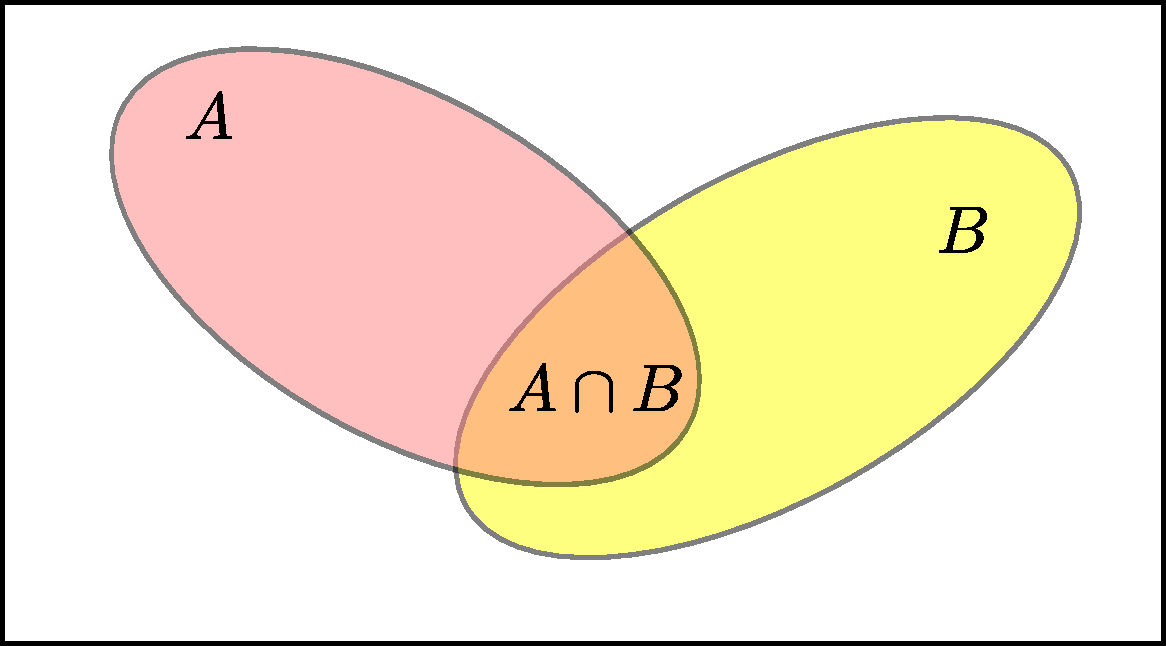
\includegraphics[width=7cm]{figs/fig-Muestra-A-B.pdf}
\caption{Dos conjuntos y su intersecci'on.}
\end{center}
\label{fig-A-B}
\end{figure}
\begin{equation}
P(A\cup B)=P(A)+P(B)-P(A\cap B).
\end{equation}

\paragraph{Ejemplo:} Se realiza un experimento para determinar el valor de dos magnitudes f'isicas. El n'umero de mediciones son 940, las que se distribuyen seg'un la siguiente tabla:
\begin{table}[h!]
\begin{center}
\begin{tabular}{cc|cc}
 & $Y$ & $C$ & $D$ \\ 
$X$ &  &  &  \\ 
\hline 
$A$ &  & 514 & 68 \\ 
$B$ &  & 112 & 246
\end{tabular} 
\caption{Distribuci'on de las 940 mediciones.}
\end{center}
\end{table}

Sean $E_1$ y $E_2$ los eventos definidos por:
\begin{align}
E_1 &= \left\{\text{todos los resultados donde } X=B\right\},\\
E_2 &= \left\{\text{todos los resultados donde } Y=D\right\}.
\end{align}

Calcular la probabilidad de obtener como resultado los siguientes casos:
\begin{equation}
X=B, \quad Y=D, \quad X=B\wedge Y=D, \quad X=B \vee Y=D, \quad X\neq B \vee Y\neq D.
\end{equation}
\begin{equation}
P(E_1)\approx\frac{358}{940}, \qquad P(E_2)\approx\frac{314}{940}, \qquad P(E_1\cap E_2)\approx\frac{246}{940},
\end{equation}
\begin{equation}
P(E_1\cup E_2)\approx\frac{426}{940}, \qquad P((E_1\cup E_2)')\approx\frac{514}{940}, \qquad P((E_1\cap E_2)')\approx\frac{694}{940}.
\end{equation}

Otra manera de resolver el ejercicio:
\begin{equation}
P(E_1\cup E_2)=P(E_1)+P(E_2)-P(E_1\cap E_2)\approx \frac{358}{940}+\frac{314}{940}-\frac{246}{940}=\frac{426}{940},
\end{equation}
\begin{equation}
P((E_1\cup E_2)')=1-P(E_1\cup E_2)\approx 1-\frac{426}{940}=\frac{514}{940}.
\end{equation}
\section{Probabilidad condicional}

En muchas ocasiones la probabilidad de un evento depende de algunas condiciones, como por ejemplo si otro evento a ocurrido (antes o simultaneamente). En estos casos resulta 'util el concepto de \textbf{probabilidad condicional}.

% Algunos fen'omenos tienden a ocurrir en rachas, esto hace que la probabilidad que ocurra un primer evento es menor que la probabilidad que se repita el evento u ocurra inmediatamente otro asociado al primero.
%		    
%\paragraph{Ejemplo:} Un canal de comunicaci'on digital tiene una tasa de error de un bit por cada mil transmitidos, es decir, la probabilidad que ocurra un error es de 1/1000. Aunque los errores son muy escasos, tienden a ocurrir en rachas, por lo que una vez ocurrido un error, la probabilidad que ocurra un segundo error es mayor que 1/1000. 

\paragraph{Definici'on:} La probabilidad condicional de un evento $A$ \textit{dado un evento} $B$, denotada por $P(A|B)$, es 
\begin{equation}\label{PAB}
P(A|B):=\frac{P(A\cap B)}{P(B)},
\end{equation}
de modo que 
\begin{equation}\label{PAyB}
P(A\cap B)=P(A|B)\cdot P(B).
\end{equation}
En palabras: ``la probabilidad de que ocurra $A$ y $B$ es igual a la probabilidad de que ocurra $A$ \underline{\textit{dado}} $B$, multiplicada por la probabilidad de que ocurra $B$".

%Consideremos un caso en que todos los resultados de un experimentos aleatorio son igualmente probables. Si existe un total de $n$ resultados
%\begin{equation}
%P(B)=\frac{(\#\text{ de resultados en }B)}{n},
%\end{equation}
%\begin{equation}
%P(A\cap B)=\frac{(\#\text{ de resultados en }A\cap B)}{n},
%\end{equation}
%\begin{equation}
%\frac{P(A\cap B)}{P(B)}=\frac{(\#\text{ de resultados en }A\cap B)}{(\#\text{ de resultados en }B)} = \text{frecuencias relativas},
%\end{equation}

Decimos que $A$ y $B$ son \textbf{eventos independientes} si se tiene que
\begin{equation}
P(A|B)=P(A), 
\end{equation}
es decir, que el resultado de $B$ no influye en la probabilidad de obtener $A$. En este caso  \eqref{pAyB} implica que
\begin{equation}\label{pAyB}
P(A\cap B)=P(A)\cdot P(B),
\end{equation}
y adem'as que
\begin{equation}
P(B|A)=P(B).
\end{equation}


\begin{figure}[h!]
\begin{center}
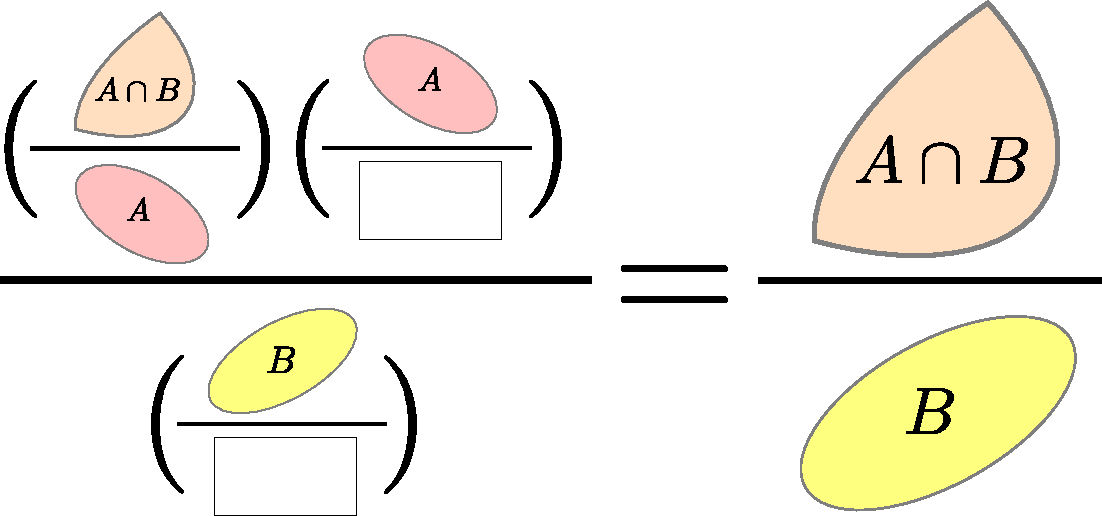
\includegraphics[width=7cm]{figs/fig-P-A-B.pdf}
\caption{Representaci'on diagram'atica de la Probabilidad condicional \eqref{PAB}.}
\end{center}
\label{fig-P-A-B}
\end{figure}
\textbf{Ejemplo:} Suponga que medimos la presencia de los contaminantes $A$ y $B$ en muestras de vino. Medimos 266 muestras de vino, las cuales arrojan el siguiente resultado: 
\begin{table}[h!]
\begin{center}
\begin{tabular}{cc|cc}
 & $A$ & S'i & No \\ 
$B$ &  &  &  \\ 
\hline 
S'i &  & 12 & 18 \\ 
No &  & 24 & 212
\end{tabular} 
\caption{Contaminantes en muestras de vino.}
\end{center}
\end{table}
\begin{equation}
P(B|A)=\frac{P(B\cap A)}{P(A)}\approx\frac{\frac{12}{266}}{\frac{36}{266}}=\frac{12}{36}=\frac{1}{3}\approx 0.33.
\end{equation}
Calculemos $P(A)$ y $P(A|B)$ para construir un diagrama, llamado diagrama 'arbol, y as'i poder comprender mejor lo que est'a pasando.
\begin{figure}[h!]
\begin{center}
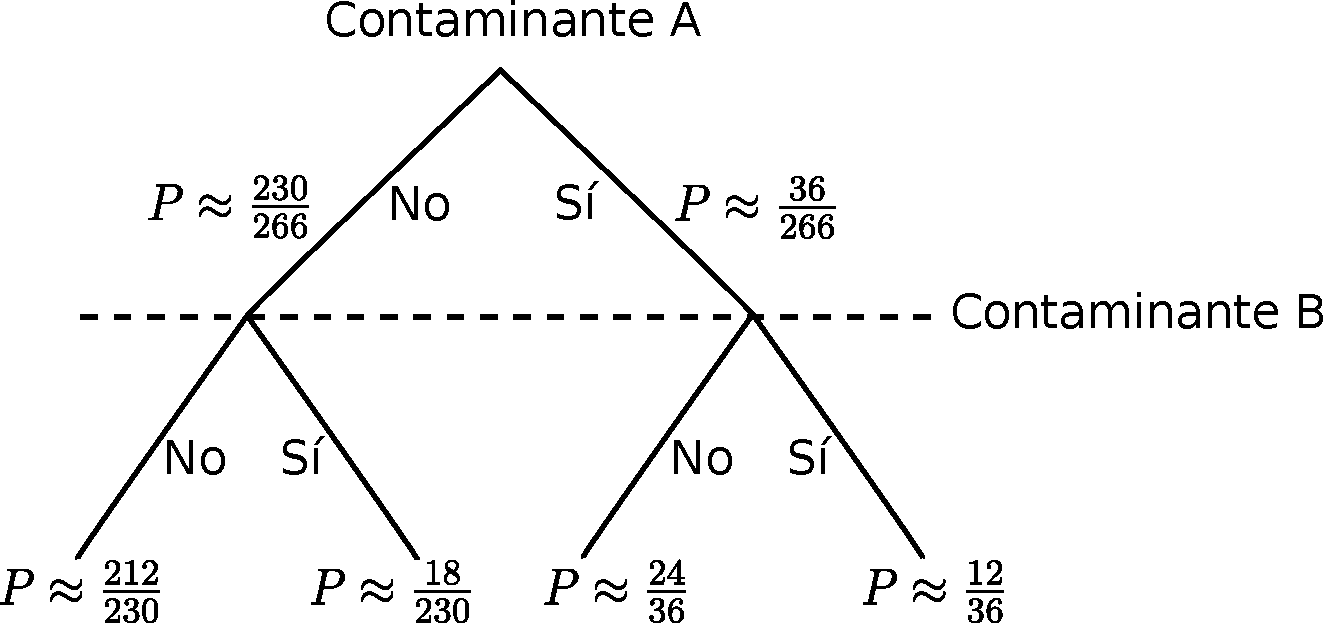
\includegraphics[width=10cm]{figs/fig-arbol.pdf}
\caption{Diagrama 'arbol.}
\end{center}
\label{fig-arbol}
\end{figure}
%Para procesos independientes la probabilidad que ocurra un evento $A$ cuando ya ha ocurrido otro evento $B$ con anterioridad, es simplemente igual a la probabilidad de $A$ (independiente de lo que pase con el evento $B$). 

%\paragraph{Definici'on:} Dos eventos son independientes si, y s'olo si, cualquiera de las proposiciones es verdadera.
%\begin{itemize}
%\item $P(A|B)=P(A)$.
%\item $P(B|A)=P(B)$.
%\item $P(A\cap B)=P(A)P(B)$.
%\end{itemize}




\subsection{Reglas de multiplicaci'on}
Como vimos, la definici'on \eqref{PAB} de probabilidad condicional implica la relaci'on \eqref{PAyB}. Esta regla de multiplicaci'on puede ser extendida a un n'umero finito de eventos ${A_i}$:
\begin{equation}
P({\bigcap^k_{i=1} A_i})=P(A_1)P(A_2|A_1)P(A_3|A_1\cap A_2)\cdots P(A_n|\bigcap^{k-1}_{i=1} A_i).
\end{equation}

\subsection{Reglas de Probabilidad total}

Cualquier evento puede escribirse como la uni'on de la parte de $B$ que se encuentra en $A$ m'as la parte de $B$ que est'a en el complemento de $A$.
(Ver figura)
\begin{equation}
B=(A \cap B) \cup (A'\cap B).
\end{equation}
Note que $(A \cap B)$ y $(A'\cap B)$ son mutuamente excluyentes. Si calculamos la probabilidad del evento $B$ usando la propiedad de uni'on y la regla de multiplicaci'on obtenemos:
\begin{equation}
P(B)=P(A \cap B)+P(B \cap A')=P(B|A)P(A)+P(B|A')P(A').
\end{equation}

\begin{figure}[h!]
\begin{center}
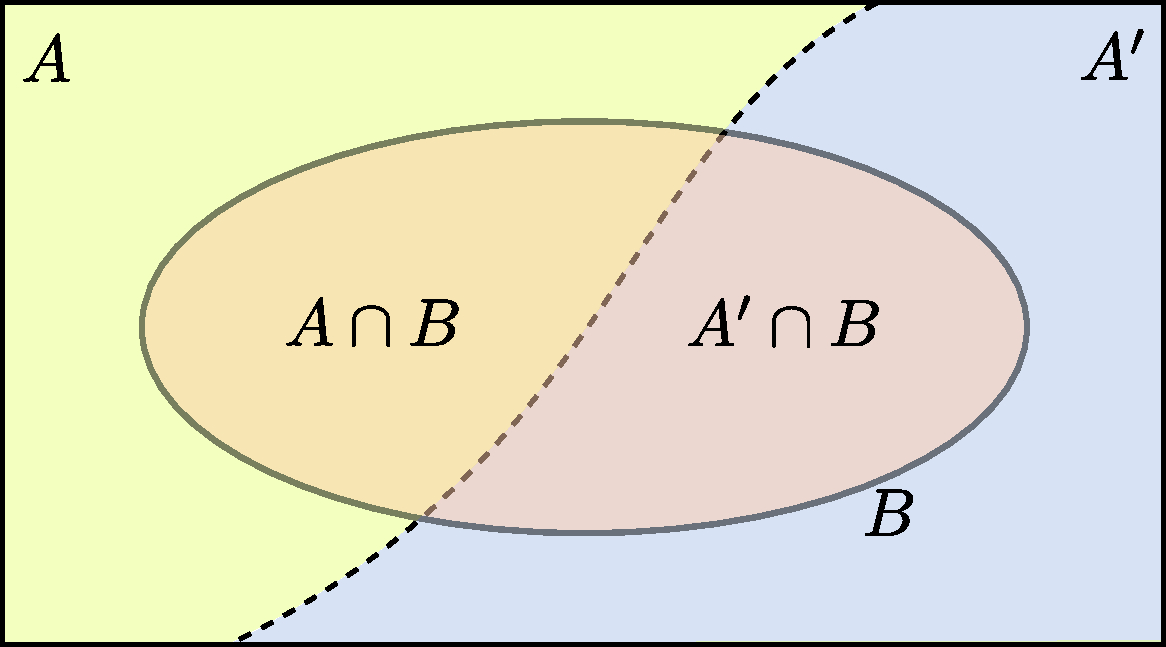
\includegraphics[width=6cm]{figs/fig-conjuntos.pdf}
\caption{Diagrama de Venn para la probabilidad total.}
\end{center}
\label{fig-conjuntos}
\end{figure}

\subsection{Teorema de Bayes}
Retomando la definici'on de probabilidad condicional \eqref{PAB} y las reglas de multiplicaci'on, es directo probar que:
\begin{equation}
P(A|B)=\frac{P(B|A)P(A)}{P(B)}.
\end{equation}
Este resultado es de gran utilidad ya que permite determinar $P(A|B)$ en funci'on de $P(B|A)$.


\textbf{Ejemplo:} Supongamos que mediante un an'alisis de 84 muestras se detectan 36 muestras con Pb, 28 con As, 12 con ambos elementos pesados y 32 est'an libres de contaminaci'on. Calcular la probabilidad de encontrar Pb entre las muestras que presentaron As: $P(\text{Pb}|\text{As})$.

\begin{table}[h!]
\begin{center}
\begin{tabular}{cc|cc}
& Pb & No & S'i \\ 
As & & & \\
\hline 
No & & 32 & 24 \\ 
S'i & & 16 & 12
\end{tabular} 
\caption{Pb y As en 84 muestras de vino.}
\end{center}
\end{table}

Usando el teorema de Bayes tenemos que
\begin{equation}
P(\text{Pb}|\text{As})= \frac{P(\text{As}|\text{Pb})P(\text{Pb})}{P(\text{As})},
\end{equation}
\begin{equation}
P(\text{Pb}|\text{As})\approx \frac{\frac{12}{36} \frac{36}{84}}{\frac{28}{84}}=\frac{12}{28}= \frac{3}{7}\approx 0.43.
\end{equation}
%Si se conocen los siguientes datos $P(\text{As}|\text{Pb})\approx 0.33$, $P(\text{Pb})\approx 0.43$, $P(\text{As})\approx 0.33$, calcular $P(\text{Pb}|\text{As})$. Usando el teorema de Bayes el c'alculo es muy simple, 
%\begin{equation}
%P(\text{Pb}|\text{As})\approx \frac{0.33 \times 0.43}{0.33}=0.43.
%\end{equation}




\section{Variables aleatorias}

\paragraph{Definici'on:} Sea $S=\{s_1,s_2,\dots,s_D\}$ un espacio muestral, cuyos elementos $s_\alpha$ ($\alpha=1,\cdots,D$) representan los posibles resultados distintos de un experimento aleatorio. Sea $X$  una funci'on de valor real definida sobre $S$, de manera que asocie los resultados de $S$ a valores reales. Se dice entonces que $X$ es una \textbf{variable aleatoria} definida sobre el espacio muestral. Entonces $S$ es el dominio de la variable aleatorio $X$ y el rango de esta funci'on es el conjunto de valores reales $\{x_\alpha=X(s_\alpha)\}$.

Decimos que la variable $X$ es \textbf{discreta} si su rango es un conjunto discreto (finito o infinito numerable) de n'umeros reales, en caso contrario decimos que $x$ es una variable \textbf{continua}.

\begin{figure}[h!]
\begin{center}
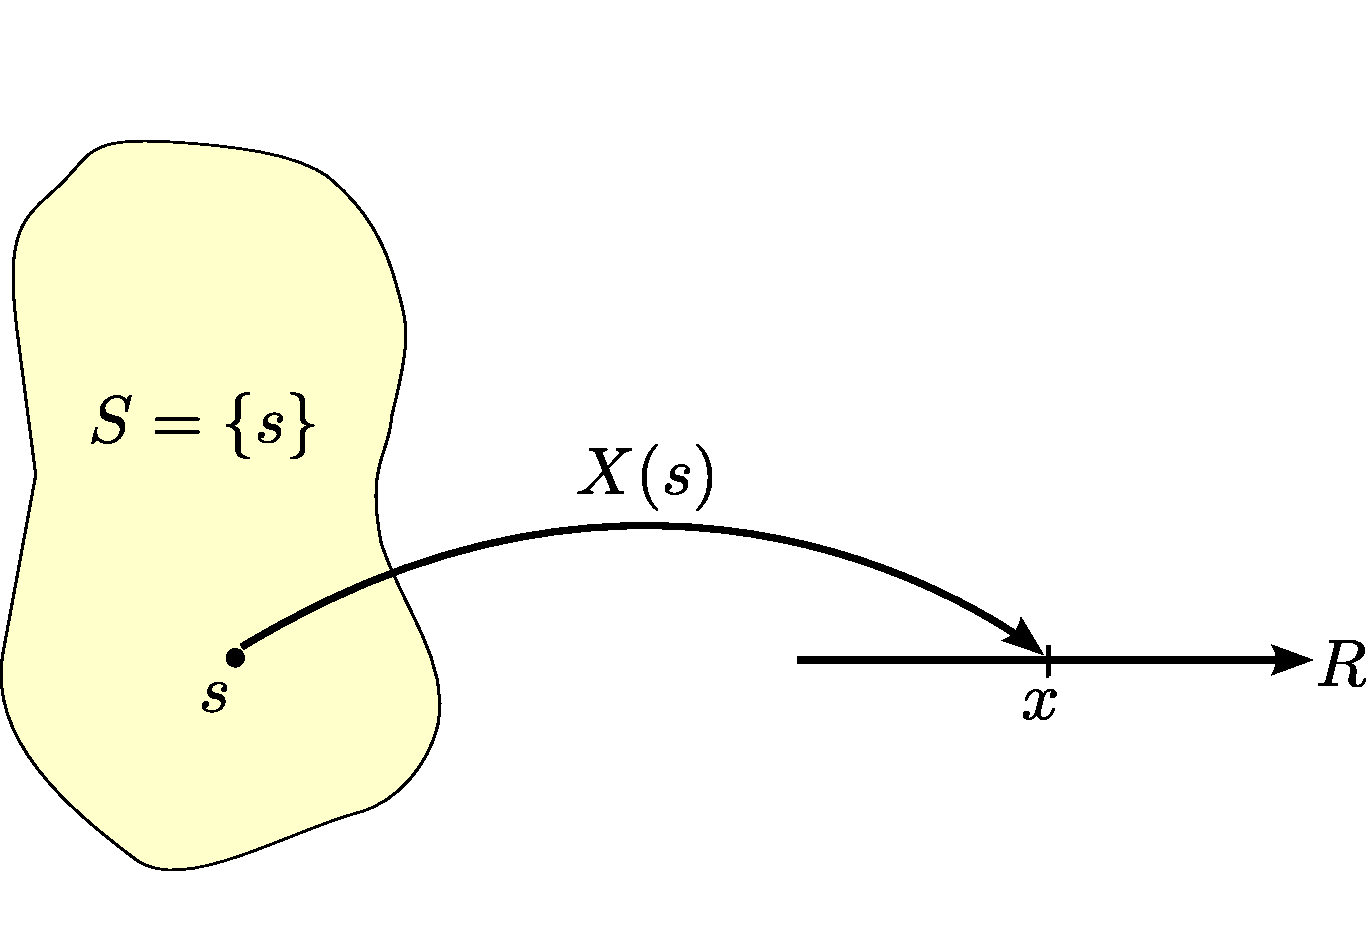
\includegraphics[width=6cm]{figs/fig-esp-muestral.pdf}
\caption{Espacio Muestral, funci'on aleatoria y rango.}
\end{center}
\label{fig-esp-muestral}
\end{figure}

Denotaremos al conjunto de todos los \textit{valores distintos} de $\{x_\alpha\}$ por $\{x_a\}$, con $a=1,\cdots, d$. Note que, si la funci'on aleatoria asigna el mismo valor real a al menos dos elementos del espacio muestral, entonces $d\le D$.

\section{Histogramas}

Luego de realizar un experimento aleatorio, se tiene un conjunto de resultados. 
%Se busca una forma de representar apropiadamente c'omo se distribuyen estas medidas.
%La idea es presentar los resultados de la mejor forma posible para poder tener una idea de como se distribuyen los datos en funcion de todos los valores distintos que puede tomar la variable aleatoria. 
Una de las mejores maneras de representar gr'aficamente la distribuci'on de los resultados es construir un \textbf{histograma}, es decir, un gr'afico de frecuencias (o n'umero de ocurrencias) para cada valor distinto de la variable aleatoria (los $\{x_a\}$).

 Como primer paso se divide el conjunto de valores de la variable aleatoria en un cierto n'umero de intervalos (intervalos de clase o celdas). Luego se grafica en el eje de las ordenadas los intervalos de clase y en el eje de las abscisas el número de veces que los resultados están contenidos en cada uno de los respectivos intervalos. Otra forma de representar los resultados es mediante un gr'afico de \textbf{frecuencias relativas}, que se diferencia del anterior en que en el eje de las abscisas ahora se grafica las frecuencias divididas por el n'umero total de datos.
%  De esta manera las frecuencias relativas son la probabilidad que la variable aleatoria tome cierto valor \textit{en la muestra} (y que se espera que sea un buen estimador de la probabilidad de la poblaci'on).

\paragraph{Ejemplo:} Arrojemos dos dados y para cada lanzamiento sumemos las dos caras superiores. Luego de repetir este experimento 100.000 veces, construyamos un histograma y un gr'afico de frecuencias relativas a partir de los datos experimentales. En este caso el gr'afico de frecuencias relativas nos permite estimar c'omo es la distribución de probabilidades de la variable aleatoria.
\begin{table}[h!]
\begin{center}
\begin{tabular}{c|c|c|c|c|c|c|c|c|c|c|c}
$x_\alpha$ & 2 & 3 & 4 & 5 & 6 & 7 & 8 & 9 & 10 & 11 & 12 \\ \hline
$n_\alpha$ & 2703 & 5526 & 8320 & 11205 & 13685 & 16778 & 13870 & 11173 & 8517 & 5511 & 2712
\end{tabular} 
\caption{N'umero de ocurrencias de cada valor de la suma de dos dados. Experimento (simulado) con $10^5$ repeticiones.}
\label{tab-suma-1E5}
\end{center}
\end{table}
\begin{figure}[h!]
\begin{center}
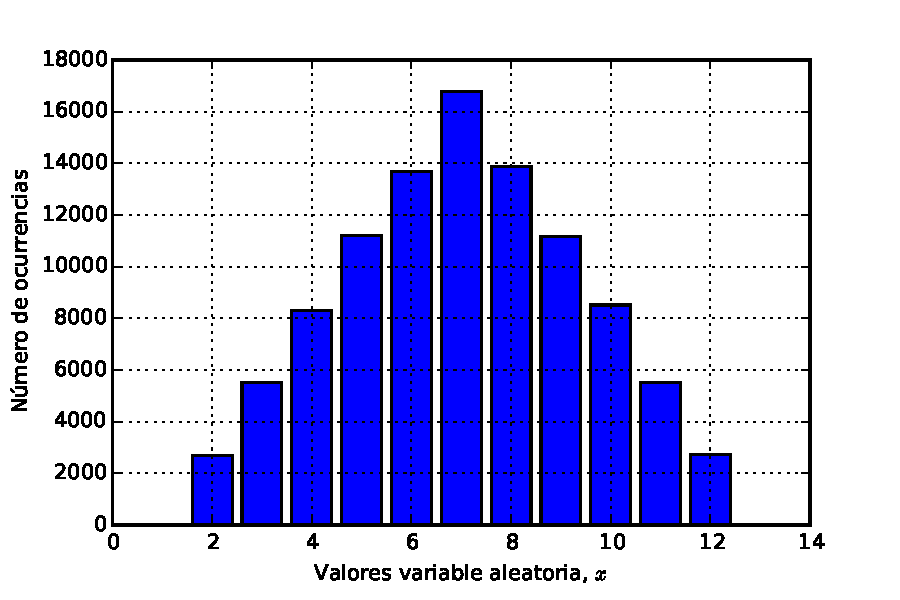
\includegraphics[width=9cm]{figs/fig-barras-dados-1E5.pdf}
\caption{Histograma de valores de suma de dados, de acuerdo a los datos en la tabla \ref{tab-suma-1E5}. C'odigo Python \href{https://github.com/gfrubi/Lab/blob/master/python/fig-conteo-suma-dados.py}{aqu\'i}.}
\end{center}
\label{fig-his-dados-1E5}
\end{figure}
\begin{figure}[h!]
\begin{center}
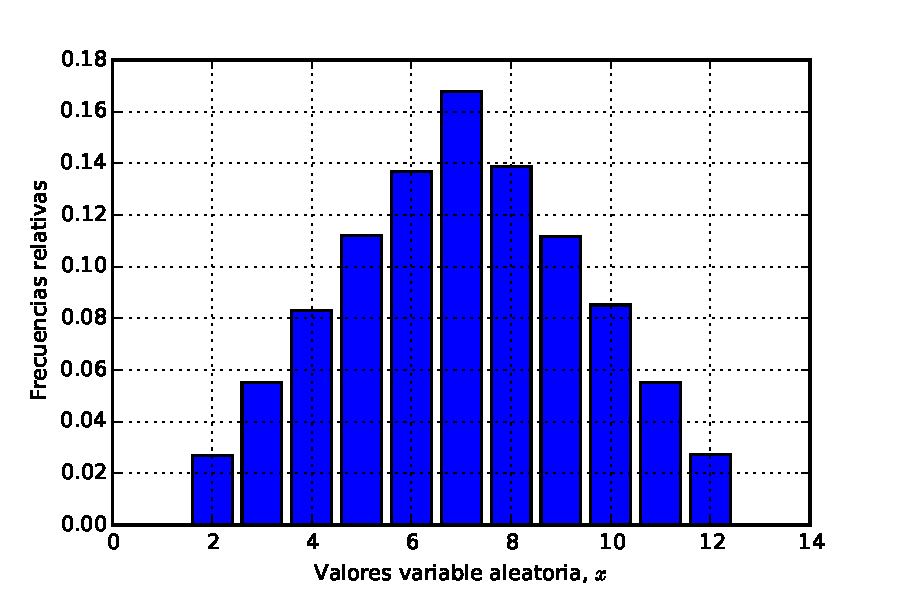
\includegraphics[width=9cm]{figs/fig-frec-relativas-dados-1E5.pdf}
\caption{Frecuencias relativas de ocurrencia de los valores de suma de dados.  C'odigo Python \href{https://github.com/gfrubi/Lab/blob/master/python/fig-frec-relativas-suma-dados.py}{aqu\'i}.}
\end{center}
\label{fig-frec-relativas-dados-1E5}
\end{figure}


\section{Distribuciones de probabilidad}
		 
 Ahora consideraremos un \textit{modelo idealizado} del experimento de los dados (de 6 caras, no cargados). Considere todos los posibles resultados al lanzar estos dos dados. Luego, definamos nuestra variable aleatoria como la suma de las caras de ambos dados, despu'es de ser arrojados. Para este caso el espacio muestral est'a formado por los $D=36$ posibles resultados, \textit{que supondremos igualmente probables}, y para los cuales la variable aleatoria puede tomar $d=11$ valores distintos. Adem'as, existe un cierto n'umero de combinaciones distintas de los resultados de cada dado que generan el mismo valor de la variable aleatoria (la suma), como se muestra en la Tabla \ref{tab-e-m}. Podemos construir un gr'afico de barras del n'umero de combinaciones en funci'on de los valores que toma la variable aleatoria. En este ejemplo, ver figura \ref{fig-bem}, el gr'afico muestra la distribuci'on de combinaciones asociadas a la variable aleatoria. M'as a'un, normalizando este gr'afico respecto al n'umero total de combinaciones (36 en este ejemplo), encontramos un gr'afico de la \textbf{distribuci'on de probabilidad} asociada a cada uno de los posibles valores de la variable aleatoria. Ver figura \ref{fig-probabilidad-dados}.
\begin{table}[h!]
\begin{center}
\begin{tabular}{|c|c|c|}
\hline 
Espacio muestral, $S$ & Valor de la variable & n'umero de  \\ 
(resultados posibles) & aleatoria, $X$ & combinaciones \\ \hline 
$(1,1)$ & 2 & 1 \\ \hline 
$(1,2)$, $(2,1)$ & 3 & 2 \\ \hline 
$(1,3)$,$(2,2)$,$(3,1)$ & 4 & 3 \\ \hline 
$(1,4)$, $(2,3)$, $(3,2)$,$(4,1)$ & 5 & 4 \\ \hline 
$(1,5)$, $(2,4)$, $(3,3)$, $(4,2)$,$(5,1)$ & 6 & 5 \\ \hline 
$(1,6)$,$(2,5)$,$(3,4)$,$(4,3)$,$(5,2)$,$(6,1)$ & 7 & 6 \\ \hline 
$(2,6)$,$(3,5)$,$(4,4)$,$(5,3)$,$(6,2)$ & 8 & 5 \\ \hline 
$(3,6)$,$(4,5)$,$(5,4)$,$(6,3)$ & 9 & 4 \\ \hline 
$(4,6)$,$(5,5)$,$(6,4)$ & 10 & 3 \\ \hline 
$(5,6)$,$(6,5)$ & 11 & 2 \\ \hline 
$(6,6)$ & 12 & 1 \\ \hline 
\end{tabular} 
\caption{N'umero de combinaciones correspondientes a cada valor de la suma de dos dados. En este caso $d=11$.}
\label{tab-e-m}
\end{center}
\end{table}
\begin{figure}[h!]
\begin{center}
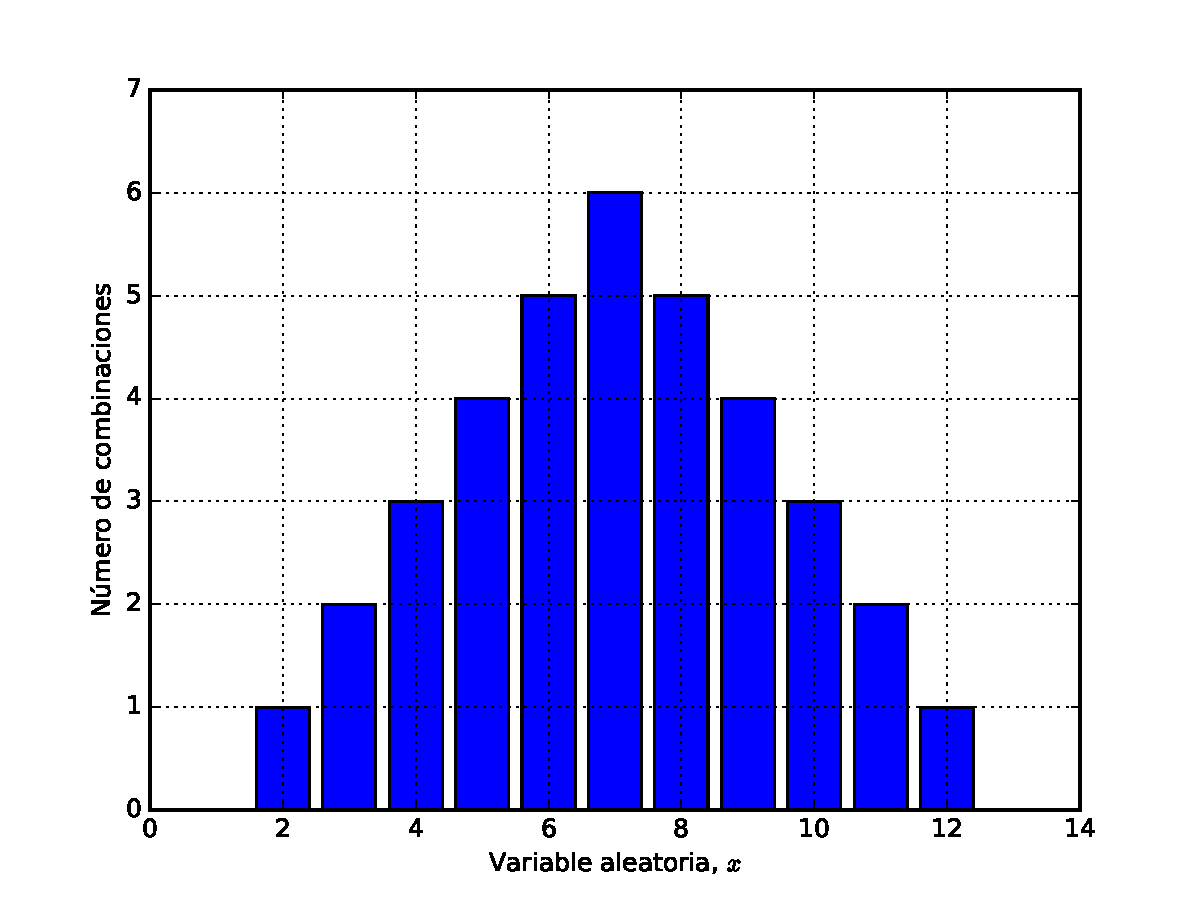
\includegraphics[width=9cm]{figs/fig-combinaciones-suma-dados.pdf}
\caption{Gr'afico de barras para los valores $x$ de la variable aleatoria, de acuerdo a los datos en la tabla \ref{tab-e-m}. C'odigo Python \href{https://github.com/gfrubi/Lab/blob/master/python/fig-combinaciones-suma-dados.py}{aqu\'i}.}
\end{center}
\label{fig-bem}
\end{figure}


\begin{figure}[h!]
\begin{center}
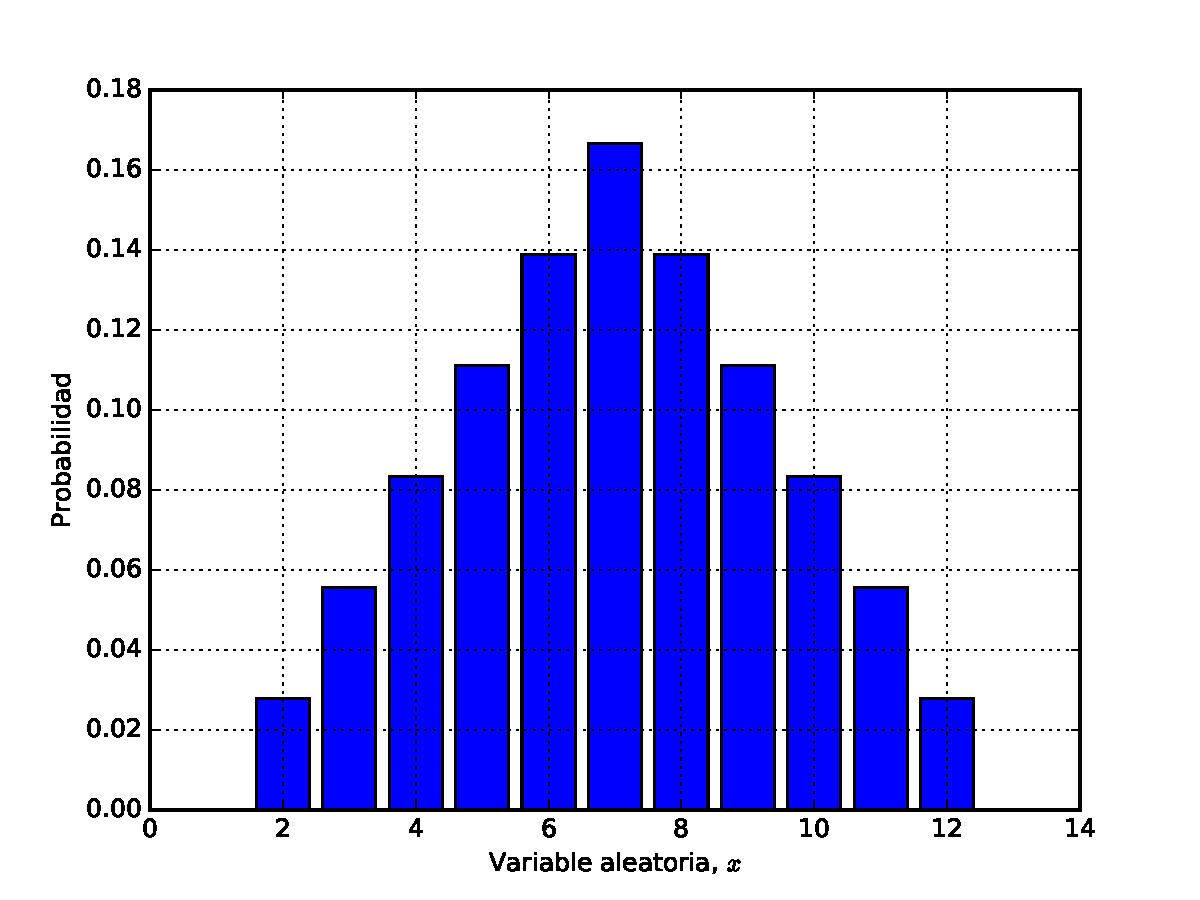
\includegraphics[width=9cm]{figs/fig-probabilidad-suma-dados.pdf}
\caption{Probabilidad para las sumas de las dos caras de dos dados. C'odigo Python \href{https://github.com/gfrubi/Lab/blob/master/python/fig-probabilidad-suma-dados.py}{aqu\'i}.}
\end{center}
\label{fig-probabilidad-dados}
\end{figure}


 Como se desprende del ejemplo, si la variable aleatoria est'a claramente definida, es posible definir una funci'on que asigne una probabilidad que dicha variable tome un determinado valor. En este caso, esta probabilidad es proporcional al n'umero de combinaciones del espacio muestral asociados a un mismo valor de la variable aleatoria. La mencionada funci'on recibe el nombre de \textbf{funci'on distribuci'on de probabilidad} de la variable aleatoria $X$. El t'ermino m'as general, \textbf{distribuci'on de probabilidad}, se refiere no s'olo a la funci'on de probabilidad, sino tambi'en a la \textbf{funci'on de distribuci'on acumulativa} de $X$, que definiremos m'as adelante.


%\paragraph{Definici'on:} Llamamos \textbf{evento} ($E$, $E\subseteq S$) a un conjunto de posibles resultados de un experimento aleatorio (Por ejemplo, el evento $E$ puede ser el conjunto de todos los resultados tales que la variable aleatoria sea par). Denotamos por $P(E)$ a la probabilidad de ocurrencia de este evento. (En nuestro ejemplo, $P(E)=P(x=2)+P(x=4)+P(x=6)+\cdots +P(x=12)$).


\paragraph{Definici'on:} La \textbf{funci'on de probabilidades} $p_X$ para una variable aleatoria discreta $X$ est'a definida como el conjunto $p_X=\{p_a\}$ de todas las probabilidades de ocurrencia de cada valor posible $x_a$ de la variable aleatoria, con
\begin{equation}
p_a=P(X=x_a) , \qquad   a=1,\cdots, d,
\end{equation}
y debe satisfacer las siguientes condiciones:
\begin{equation}
p_a\geq 0, \qquad  a=1,\cdots, d,
\end{equation}
\begin{equation}
\sum_{a=1}^d p_a=1.
\end{equation}
		 
\paragraph{Definici'on:} La \textbf{funci'on de distribuci'on acumulativa} (``cumulative distribution function'', cdf) de una variable aleatoria discreta $X$, es la probabilidad que el valor de $X$ sea menor o igual a un valor especifico $x$ y est'a dado por:
\begin{equation}
F_X(x)=P(X\le x)=\sum_{x_a\le x}p_X(x_a)=\sum_{x_a\le x}p_a.
\end{equation}
		
Como consecuencia, la probabilidad de que la variable $X$ \textit{adopte un valor mayor que $x$} es
\begin{equation}
P(X> x) = 1 - F_X(x),
\end{equation}
y la probabilidad de que la variable $X$ \textit{adopte un valor mayor que $a$ y menor o igual a $b$}, es decir, en el intervalo $(a,b]$ es
\begin{equation}
P(a<X\le b) = F_X(b)-F_X(a).
\end{equation}
%	Por lo tanto, en el caso discreto, una variable aleatoria est'a caracterizada por la funci'on de probabilidad $p_a$, la cual determina la probabilidad puntual que $X = x_a$ , y por la funci'on distribuci'on acumulativa $F(x)$, la que representa la suma de las probabilidades puntuales hasta el valor $x$ de $X$, inclusive.
%		 
%Una caracter'istica importante del an'alisis de datos, es c'omo se distribuyen 'estos alrededor del valor medio. Un histograma, como hemos visto, proporciona una representaci'on visual simple de tal distribuci'on. 
 
%aqu'i presentaremos dos de los ejemplos m'as comunes de distribuciones. 
%
%\begin{enumerate}
%\item Distribuci'on de Poisson.
%\item Distribuci'on de Gauss.
%\end{enumerate}

\subsection{Distribuciones de Poisson}

\paragraph{Ejemplo:} Se tiene una muestra de material radiactivo y se registra el n'umero de part'iculas emitidas en los decaimientos (por ejemplo, usando un contador Geiger). El contador registra el n'umero de decaimientos detectados y 'estos tienen un comportamiento aleatorio, en el sentido que no puede ser predicho cu'ando ocurrir'a el siguiente decaimiento. Luego de detectadas las part'iculas emitidas, podemos realizar un conteo del n'umero $x$ de decaimientos registrados en cada intervalo de tiempo de largo $\Delta t$ (por ejemplo, en cada intervalo de $\Delta t=3 {\rm s}$). Entonces $x$ es una variable aleatoria discreta que puede asumir los valores $x=0, 1,2,\dots$, que tomar'an valores distintos en cada intervalo $\Delta t$. Luego de muchas mediciones, podemos realizar el conteo de cu'antas veces se detectaron $x$ part'iculas en el intervalo $\Delta t$. Si denotamos como $n(x)$ al n'umero de veces que se detectaron $x$ part'iculas (en intervalos de largo $\Delta t$), entonces podemos construir un histograma $n(x)$ versus $x$, y el gr'afico de frecuencias relativas $n(x)/N$ versus $x$, donde $N=\sum_{x=1}^\infty n(x)=n(0)+n(1)+n(2)+\cdots$ es el n'umero total de mediciones realizadas (en este ejemplo, el n'umero total de intervalos de largo $\Delta t$ en los que se realiz'o el conteo). Finalmente, en el l'imite $N\to\infty$ el gr'afico $n(x)/N$ versus $x$ tiende al gr'afico de distribuci'on de probabilidad de medir $x$ part'iculas en un intervalo (de largo $\Delta t$). Bajo algunas hip'otesis (que revisaremos a continuaci'on) podemos modelar 'este tipo de casos (y muchos otros) usando una \textbf{distribuci'on probabilidad de Poisson}, que est'a caracterizada por un 'unico par'ametro $\mu$.
%\begin{figure}[h!]
%\begin{center}
%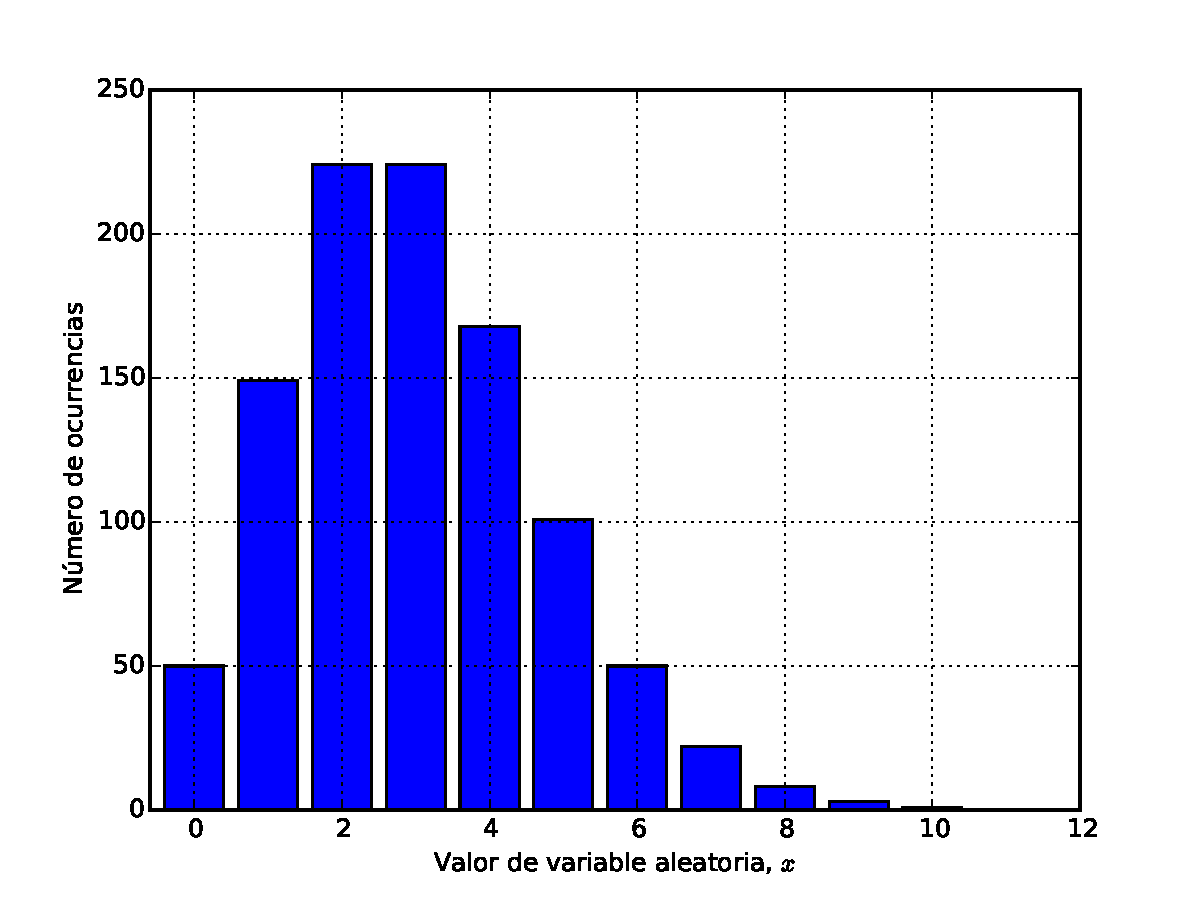
\includegraphics[width=9cm]{figs/fig-Poisson.pdf}
%\caption{n'umero de part'iculas $\alpha$ emitidas en un intervalo de tiempo dado. C'odigo Python en ap'endice \ref{app-Poisson}.}
%\end{center}
%\label{fig-Poisson}
%\end{figure}
\begin{figure}[h!]
\begin{center}
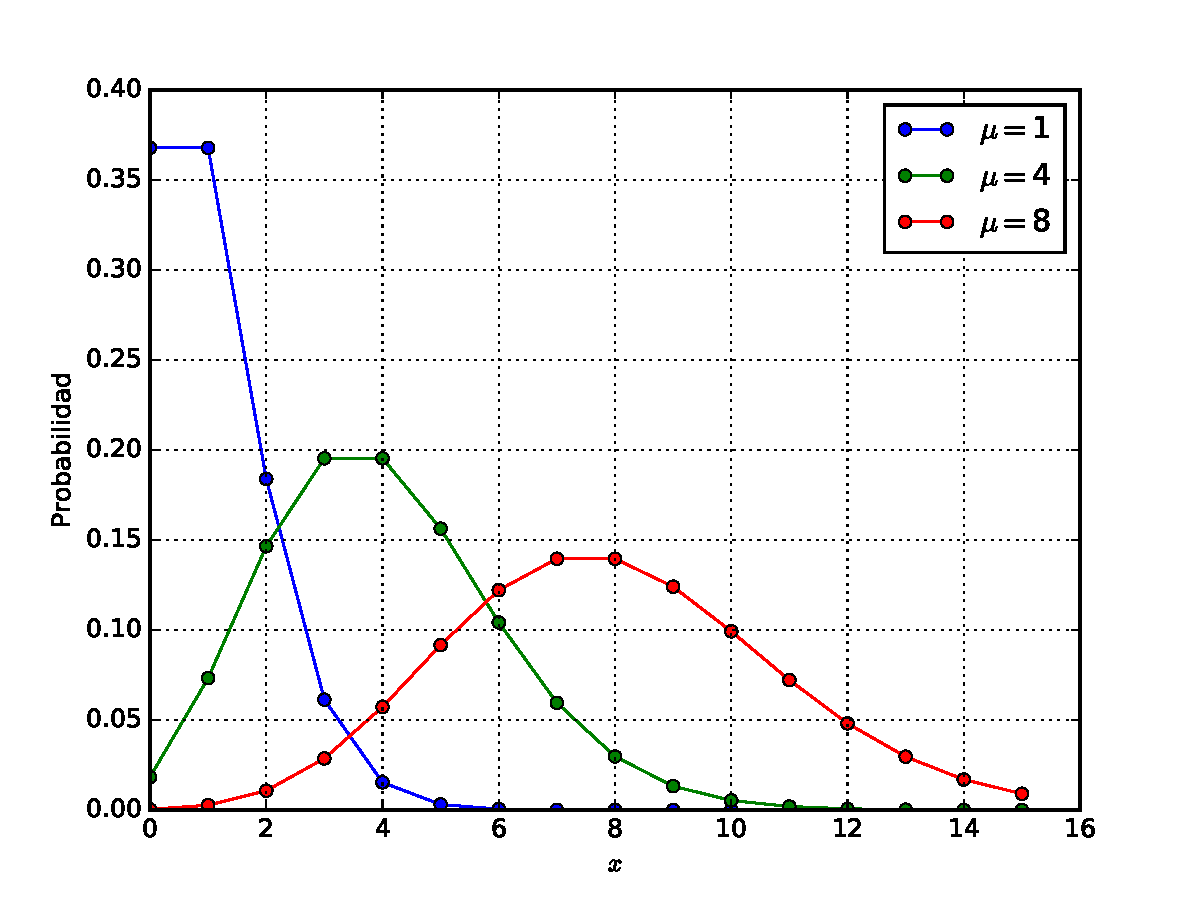
\includegraphics[width=9cm]{figs/fig-probabilidad-Poisson.pdf}
\caption{Funci'on probabilidad de Poisson. C'odigo Python \href{https://github.com/gfrubi/Lab/blob/master/python/fig-probabilidad-Poisson.py}{aqu\'i}.}
\end{center}
\label{fig-probabilidad-Poisson}
\end{figure}
\paragraph{Definici'on:} Sea $X$ una variable aleatoria que representa el n'umero de eventos aleatorios independientes que ocurren en un cierto intervalo (de tiempo, espacio, etc.). Se dice entonces que la variable aleatoria $X$ tiene una \textbf{distribuci'on de Poisson} si su  funci'on de probabilidad es dada por
\begin{equation}
P(x,\mu)=\frac{e^{-\mu}\mu^x}{x!}, \qquad x=0,1,2,3,\cdots,\quad \mu>0 .
\end{equation}
El par'ametro $\mu$ de la distribici'on es el \textbf{n'umero medio de sucesos esperados} (n'umero promedio de ocurrencias del evento en el intervalo de observaci'on, ya sea tiempo, distancia, etc.). Esta distribuci'on de probabilidad satisface las siguientes propiedades:
\begin{itemize}
\item Condici'on de normalizaci'on,
\begin{equation}
\sum_{x=0}^\infty P(x,\mu)=1.
\end{equation}
\item Valor medio,
\begin{equation}
\mu_{X}=\sum_{x=0}^\infty xP(x,\mu)=\mu.
\end{equation}
\item Varianza,
\begin{equation}
\sigma^2=\sum_{x=0}^\infty (x-\mu)^2P(x,\mu)=\mu,  
\end{equation}
\item Desviaci'on est'andar,
\begin{equation}
\sigma=\sqrt{\mu}.
\end{equation}
\end{itemize}

En general, la distribuci'on de probabilidad de Poisson es el modelo matem'atico que describe procesos en los que se satisfacen las siguientes propiedades:
Se dice que el proceso es de Poisson si satisface que, al dividirse el conteo en sub-intervalos suficientemente peque\~nos:
\begin{itemize}
\item La probabilidad de \textit{ocurrencia simult'anea} de dos eventos es nula.
\item Los eventos ocurren en forma \textit{independiente}.
\item La probabilidad de ocurrencia de un evento \textit{por intervalo} (de tiempo, o distancia, etc.) es constante. Equivalentemente, la probabilidad de ocurrencia de un evento \textit{es proporcional al intervalo} (de tiempo, o distancia, etc.) de observaci'on.
\end{itemize}

En el ejemplo de los decaimientos radiactivos, las condiciones listadas arriba parecen hip'otesis razonables, por lo que esperamos que este tipo de proceso pueda modelarse apropiadamente como un proceso de Poisson. En particular, si $\nu$ es el \textbf{n'umero medio de decaimientos por unidad de tiempo}\footnote{En Mec'anica Cu'antica es usual poder calcular la \textbf{probabilidad por unidad de tiempo}, $\dot{P}_{\rm dec}$, que un n'ucleo radiactivo decaiga. En este caso, $\nu={\cal N}\dot{P}_{\rm dec}$, donde $\cal N$ es el n'umero total de n'ucleos presentes en la muestra analizada.} de que se produzca un decaimiento en el material, entonces $\mu=\nu\Delta t$ es el n'umero medio de decaimientos esperados en el intervalo de tiempo $\Delta t$.

\paragraph{Ejemplo:} Se estima que cada a\~no se producen aproximadamente 13000 sismos de magnitud mayor que 4 en el mundo. Suponiendo que 'estos se distribuyen aleatoriamente en el a\~no y que son independientes, deber'iamos este proceso sea de Poisson. Estime la probabilidad de que se produzcan 5 sismos de estas caracter'isticas durante la misma hora. % mu = 13000/365 = 35.6 sismos/dia  = 1.48 sismos/hora, p(5,1.48)*100 = 1.35%

\subsection{Distribuci'on de probabilidad de una variable aleatoria continua: densidad de probabilidad}
Cuando la variable aleatoria puede tomar cualquier valor dentro de un cierto intervalo de n'umeros reales, diremos que la variable aleatoria es \textbf{continua}.

\paragraph{Definici'on:} Una funci'on $f_X(x)$ es una \textbf{funci'on de densidad de probabilidad} de la variable aleatoria continua X si para cualquier intervalo de n'umeros reales $[x_1,x_2]$:
\begin{enumerate}
\item $f_X(x)\geq 0$,
\item $\int_{-\infty}^\infty f_X(x)\,dx=1$,
\item $P(x_1\le X\le x_2)=\int_{x_1}^{x_2}f_X(u)\,du$.
\end{enumerate}

Esto permite interpretar $f_X(x)\,dx$ como la probabilidad de que la variable $X$ asuma un valor entre $x$ y $x+dx$. Es importate recordar que $f_X(x)$ no es directamente el valor de la probabilidad sino que es la ``probabilidad por unidad de intervalo de $x$". Esto se refleja tambi'en en las unidades de medida de $f_X(x)$:
\begin{equation}
[f_X]=\frac{[P]}{[\Delta x]}=\frac{1}{[x]}.
\end{equation}
As'i, por ejemplo, si la variable aleatoria $x$ representa una distancia, entonces $[x]=L$ y $[f_X]=L^{-1}$.


\paragraph{Definici'on:} La \textbf{funci'on distribuci'on acumulada} de una variable aleatoria continua $X$ es
\begin{equation}
F_X(x)=P(X\le x)=\int_{-\infty}^x f_X(u)\,du.
\end{equation}



\paragraph{Definici'on:} Si $X$ es una variable aleatoria continua con funci'on de densidad de probabilidad $f_X(x)$, $-\infty<x<\infty$, entonces la \textbf{media} de $X$, est'a definida por
\begin{equation}
\mu=\int_{-\infty}^\infty xf_X(x)\,dx.
\end{equation}
Adem'as, la \textbf{varianza} de $X$ es definida por 
\begin{equation}
\sigma_X^2=\int_{-\infty}^\infty (x-\mu)^2f_X(x)\,dx.
\end{equation}
La \textbf{desviaci'on est'andar} es entonces
\begin{equation}
\sigma_X=\sqrt{\sigma_X^2}=\sqrt{\int_{-\infty}^\infty (x-\mu)^2f_X(x)\,dx}.
\end{equation}


\begin{figure}[h!]
\begin{center}
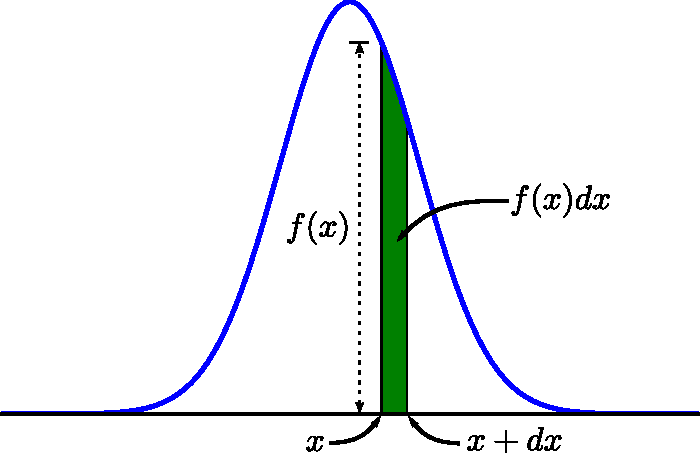
\includegraphics[width=8cm]{figs/fig-densidad-de-probabilidad.pdf}
\caption{Densidad de probabilidad.}
\end{center}
\label{fig-dens-prob}
\end{figure}
\subsection{Distribuci'on de Gauss o Normal}
	
%\paragraph{Ejemplo} 
%Al hacer estudios del poder de frenado (Stopping Power) lo que se desea describir es la p'erdida media de energ'ia de un has de part'iculas al viajar por el interior de un material. Supongamos que se hace incidir protones sobre una l'amina delgada de oro. Si graficamos la energ'ia de los protones dividida en intervalos de clase, luego que estos han atravesado la l'amina de oro, en el eje de las abscisas y el n'umero de protones correspondiente a cada intervalo en el eje de las ordenadas.

%\begin{figure}[h!]
%\begin{center}
%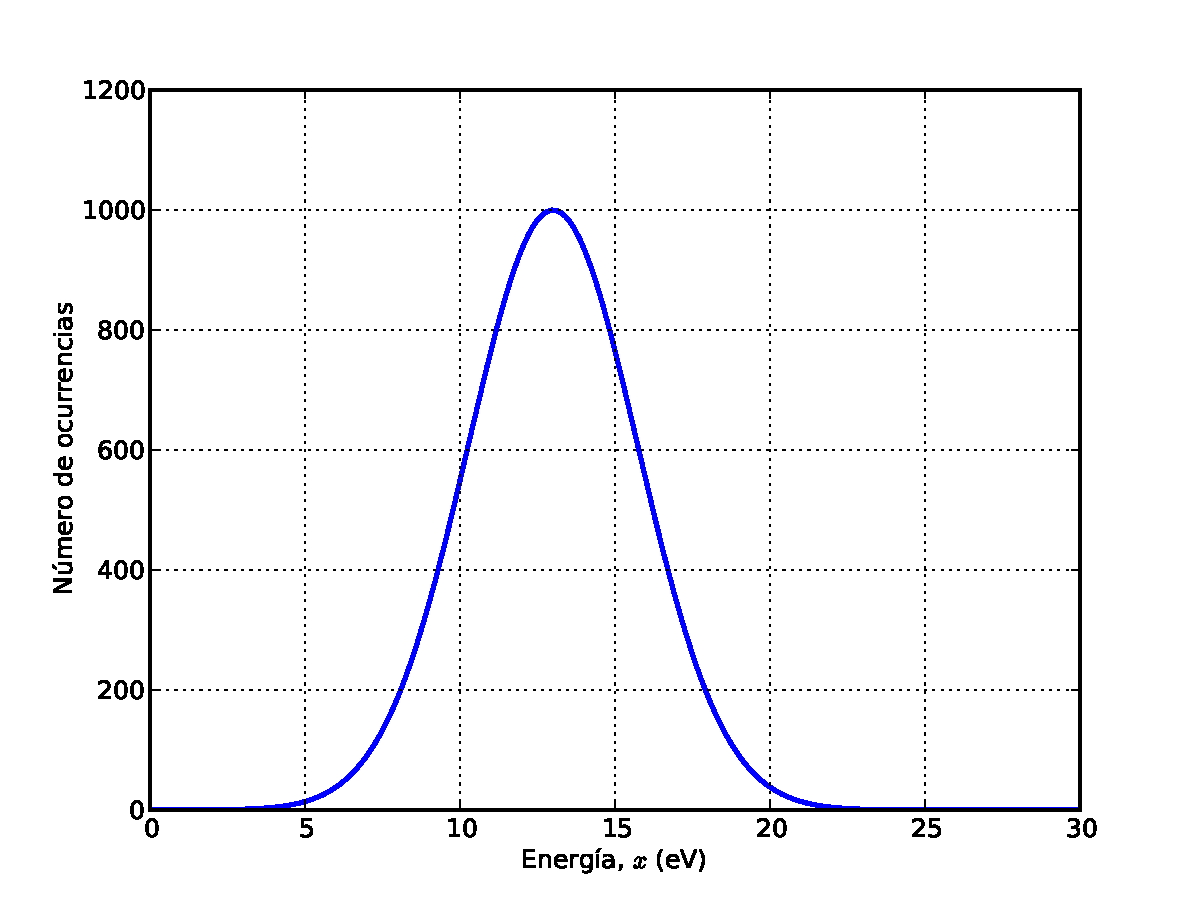
\includegraphics[width=9cm]{figs/fig-Gauss.pdf}
%\caption{P'erdida de energ'ia de protones luego de atravesar una l'amina de oro. C'odigo Python en ap'endice \ref{app-Gauss}.}
%\end{center}
%\label{fig-Gauss}
%\end{figure}

%	Retomando nuestros tres ejemplos de histogramas y normalizando cada uno de estos al n'umero total de eventos (si pensamos en t'erminos de una funci'on continua, seria normalizando al 'area de la curva)
%		


\begin{figure}[h!]
\begin{center}
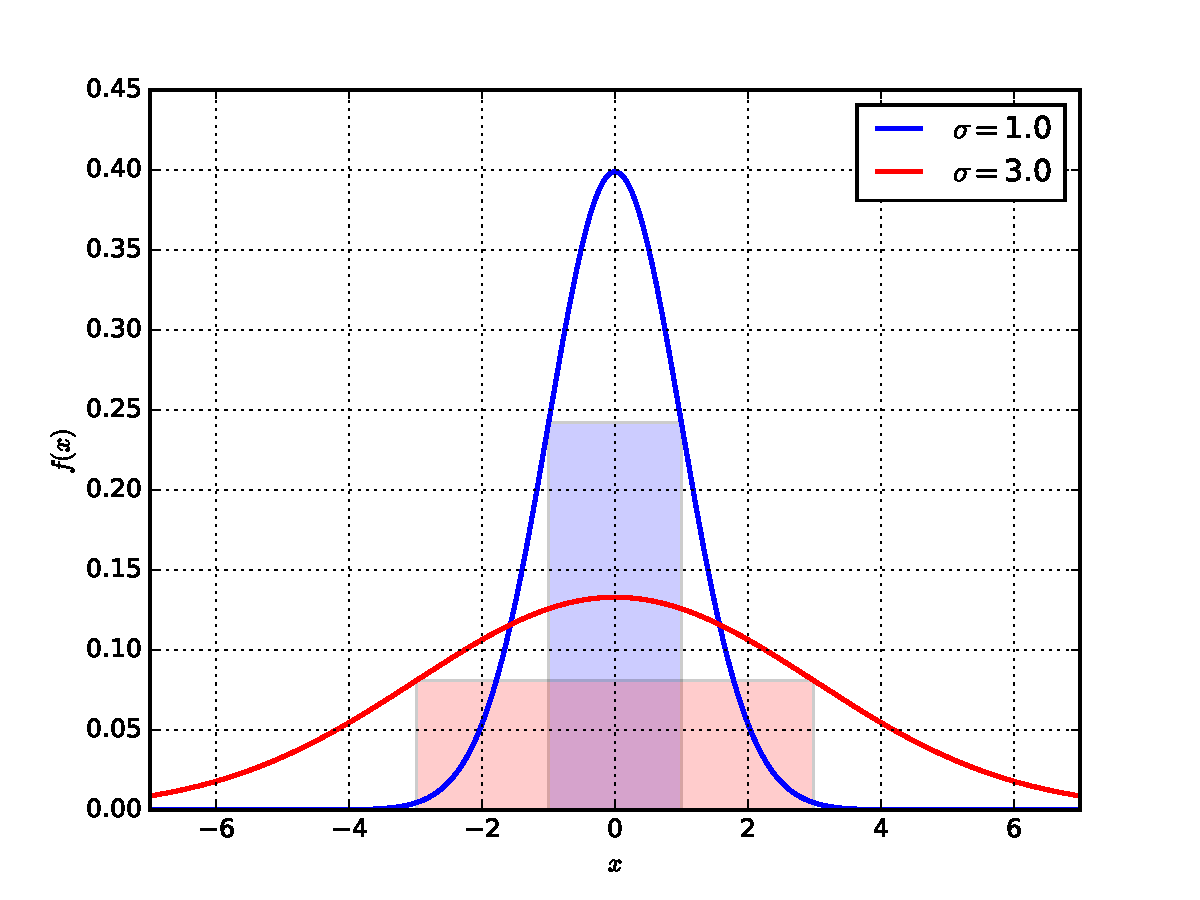
\includegraphics[width=9cm]{figs/fig-normal.pdf}
\caption{Distribuci'on normal.C'odigo Python \href{https://github.com/gfrubi/Lab/blob/master/python/fig-normal.py}{aqu\'i}.}
\end{center}
\label{fig-normal}
\end{figure}


\paragraph{Definici'on:} Se dice que una variable aleatoria $X$, se encuentra \textbf{normalmente distribuida} (Distribuci'on de Gauss) si su funci'on densidad de probabilidad est'a dada por:
\begin{equation}
f(x;\mu,\sigma)=\frac{1}{\sqrt{2\pi\sigma^2}}e^{-\frac{1}{2}\left(\frac{x-\mu}{\sigma}\right)^2}, \qquad -\infty<x<\infty,
\end{equation}
donde $-\infty<\mu<\infty$ y $\sigma>0$ denotan la media y la desviaci'on est'andar de $X$, respectivamente.  


\subsubsection{Propiedades}

Si $X$ es una variable aleatoria normal con valor medio $\bar{x}=\mu$ y varianza $\sigma_x^2=\sigma^2$, entonces la variable aleatoria
\begin{equation}
z=\frac{(x-\mu)}{\sigma}
\end{equation}
es una \textbf{variable aleatoria normal} con $\bar{z}=0$ y varianza $\sigma_z^2=1$. Esto es, $Z$ es una variable aleatoria normal est'andar.
La creaci'on de una variable aleatoria con esta transformaci'on se conoce como \textbf{estandarizaci'on}. La variable aleatoria $Z$ representa la diferencia de $X$ y su promedio, en unidades de desviaciones est'andar.

\paragraph{Utilidad de la estandariaci'on:}
Suponga que $X$ es una variable aleatoria con distribuci'on normal con media $\mu$ y varianza $\sigma^2$. Entonces,
\begin{equation}
P(X\leq x)=P\left(\frac{(X-\mu)}{\sigma} \leq \frac{(x-\mu)}{\sigma}\right)=P(Z\leq z),
\end{equation} 
donde
$Z$ es una variable aleatoria normal, y $z:=(x-\mu)/\sigma$ es el valor de $z$ obtenido a trav'es de la estandarizaci'on de $X$.

An'alogamente, es posible definir la \textbf{funci'on distribuci'on acumulada} de una variable aleatoria normal est'andar como
\begin{equation}
\Phi(z)=P(Z\leq z).
\end{equation} 

Los puntos de inflexi'on, la \textbf{media}, la \textbf{varianza} y la desviaci'on est'andar, usando la funci'on distribuci'on estandarizada, estar'ian dadas por
\begin{align}
f(x) = \frac{1}{\sqrt{2\pi\sigma^2}} e^{-\frac{1}{2}\left(\frac{x-\mu}{\sigma}\right)^2} =\frac{1}{\sqrt{2\pi\sigma^2}} e^{-\frac{1}{2}z^2},
\end{align}
%\begin{align}
%\frac{df(z)}{dz}&= \frac{-2z}{2\sqrt{2\pi\sigma^2}} e^{-z^2/2}=0 \\
%&\Rightarrow z=\frac{(x-\mu)}{\sigma}=0\\
%& x=\mu
%\end{align}
\begin{align}
\frac{d^2 f(z)}{dz^2}\stackrel{!}{=}0 \quad
\Rightarrow \quad  \frac{1}{\sqrt{2\pi\sigma^2}}e^{-z^2/2}  ( z^2 - 1 )=0 \quad 
\Rightarrow\quad z=\pm 1 \quad \Rightarrow\quad x=\mu \pm \sigma
\end{align}
\begin{align}
\bar{x} &= \frac{1}{\sqrt{2\pi\sigma^2}}\int_{-\infty}^\infty x e^{-\frac{1}{2}\left(\frac{x-\mu}{\sigma}\right)^2}dx \\
&= \frac{1}{\sqrt{2\pi}} \int_{-\infty}^\infty (\mu+\sigma z) e^{-z^2/2}dz \\
&= \frac{\mu}{\sqrt{2\pi}} \int_{-\infty}^\infty e^{-z^2/2}dz+0 \\
&= \frac{\mu}{\sqrt{2\pi}}(\sqrt{2\pi})\\
&= \mu
\end{align}
\begin{align}
\sigma_X^2 &= \frac{1}{\sqrt{2\pi\sigma^2}}\int_{-\infty}^\infty (x-\mu)^2 e^{-\frac{1}{2}\left(\frac{x-\mu}{\sigma}\right)^2}dx \\
&= \frac{1}{\sqrt{2\pi}}\int_{-\infty}^\infty (\sigma z)^2 e^{-z^2/2}dz \\
&= -\frac{\sigma^2}{\sqrt{2\pi}}\int_{-\infty}^\infty z\frac{d}{dz}\left(e^{-z^2/2}\right)dz \\
&=-\frac{\sigma^2}{\sqrt{2\pi}}\left[\left.ze^{-z^2/2}\right|_{-\infty}^\infty-\int_{-\infty}^\infty e^{-z^2/2} dz\right] \\
&=-\frac{\sigma^2}{\sqrt{2\pi}}\left[0-\sqrt{2\pi}\right] \\
&= \sigma^2.
\end{align}

\begin{align}
\sigma_x=\sqrt{\sigma_x^2}=\sigma,
\end{align}
respectivamente.



\chapter{Desviación estándar de una función de varias variables}\label{sec:propdesv}

\newpage

Supongamos que la magnitud del valor que queremos hallar, depende de las variables $x^1, x^2, \dots, x^m$  mediante la relaci'on funcional $y=f(x^\alpha)$, $\alpha=1,\dots,m$. Luego de realizar $N$ medidas para cada una de las $m$ variables, tenemos
\begin{center}
\begin{tabular}{cccccc}
%\hline 
$x^1_1$ & $x^1_2$ & $\cdots$ & $x^1_N$ & ; & $\bar{x}^1$ \\ 
%\hline 
$x^2_1$ & $x^2_2$ & $\cdots$ & $x^2_N$ & ; & $\bar{x}^2$ \\ 
%\hline 
$\vdots$ & $\vdots$ & $\vdots$ & $\vdots$ & ; & $\vdots$ \\ 
%\hline 
$x^m_1$ & $x^m_2$ & $\cdots$ & $x^m_N$ & ; & $\bar{x}^m$.
%\hline 
\end{tabular} 
\end{center}
Escribimos las desviaciones respecto al promedio como $\Delta x^1_i, \Delta x^2_i, \cdots \Delta x^m_i$, donde
\begin{equation}
\Delta x^1_i:=x_i^1-\bar{x}^1, \qquad \Delta x^2_i:=x_i^2-\bar{x}^2,
\end{equation}
etc.

Las magnitudes determinadas indirectamente, estarán dadas por cada uno de los conjuntos de medidas mediante la relaci'on funcional:
\begin{align}
y_1 &= f(x^1_1,x^2_1,\cdots, x^m_1), \\
\vdots &= \quad\vdots  \\
y_i &= f(x^1_i,x^2_i,\cdots, x^m_i),\\
\vdots &= \quad \vdots,  \\
y_N &= f(x^1_N,x^2_N,\cdots, x^m_N).
\end{align}

Desarrollando en serie de Taylor a primer orden en torno de los valores medios, podemos escribir:
\begin{align}
y_i & = f(x^1_i,x^2_i,\cdots, x^m_i)\\
&\approx  f(\bar{x}^1,\bar{x}^2,\cdots, \bar{x}^m)+ \sum_{\alpha=1}^m\left.\frac{\partial f}{\partial x^\alpha}\right|_{\bar{x}^\alpha}(\Delta x^\alpha_i).
\end{align}

Las diferencias respecto al valor de la función evaluada en el promedio de cada conjunto de mediciones se pueden expresar como
\begin{align}
\Delta y_i &:= y_i-f(\bar{x}^1,\cdots, \bar{x}^m)\\
&\approx  \sum_{\alpha=1}^m\left.\frac{\partial f}{\partial x^\alpha}\right|_{\bar{x}^\alpha}(\Delta x^\alpha_i).
\end{align}

Calculamos con esto la varianza (el cuadrado de la desviaci'on est'andar) de $y$:
\begin{align}
\sigma_y^2 &:= \sum_{i=1}^N\frac{1}{N-1}(\Delta y_i)^2 \\
&\approx \frac{1}{N-1}\left[\sum_{i=1}^N\left[\left(\left.\frac{\partial f}{\partial x^1}\right|_{\bar{x}}\right)^2 (\Delta x^1_i)^2 +\cdots + \left(\left.\frac{\partial f}{\partial x^m}\right|_{\bar{x}}\right)^2(\Delta x^m_i)^2 \right.\right. \nonumber \\
& \quad +  2\left(\left.\frac{\partial f}{\partial x^1}\right|_{\bar{x}}\right)\left(\left.\frac{\partial f}{\partial x^2}\right|_{\bar{x}}\right)(\Delta x^1_i)(\Delta x^2_i)+\cdots \nonumber\\
& \quad \left.\left.  +2\left(\left.\frac{\partial f}{\partial x^{m-1}}\right|_{\bar{x}}\right) \left(\left.\frac{\partial f}{\partial x^m}\right|_{\bar{x}}\right)(\Delta x^{m-1}_i)(\Delta x^m)\right]\right],
\end{align}
donde $\bar{x}=(\bar{x}^1,\cdots, \bar{x}^m)$.

Separamos esta 'ultima expresi'on en dos casos. 

\begin{itemize}
\item Caso 1. Cuando las variables medidas est'an correlacionadas.
Para este caso, la desviación estándar de los valores de $y$ est'a dada por la raíz cuadrada de la expresi'on que se obtuvo.

\item Caso 2. Cuando las variables medidas no están correlacionadas.
En este caso, la suma de todos los t'erminos cruzados son cero (o despreciable!), por lo que la expresi'on se reduce a
\begin{equation}
\sigma_y^2 \approx \frac{1}{N-1}\sum_{i=1}^N\left[\left(\left.\frac{\partial f}{\partial x^1}\right|_{\bar{x}}\right)^2 (\Delta x^1_i)^2 +\cdots + \left(\left.\frac{\partial f}{\partial x^m}\right|_{\bar{x}}\right)^2(\Delta x^m_i)^2\right]
\end{equation}
\end{itemize}

Una manera muy simple de visualizar que los t'erminos cruzados no contribuyen al valor de $\sigma_y^2$, consiste en observar la figura \ref{fig-dist}, donde en cada eje se grafic'o una variable distinta. Las dos im'agenes superiores, de la misma figura, son casos sin correlaci'on entre las variables medidas y las dos figuras inferiores tienen una clara correlaci'on. 
Luego, dividimos cada una de estas figuras en 4 cuadrantes. En todas las figuras el t'ermino cruzado $\sum_i(x_i^\alpha-\bar{x}^\alpha)(x_i^\beta-\bar{x}^\beta)$ (con $\alpha\neq\beta$) es positivo en los cuadrantes I y III y negativo en los cuadrantes II y IV. 
Para las dos figuras superiores, el n'umero de medidas en cada uno de los cuadrantes son iguales, por lo que la suma total de los cuatro cuadrantes ser'a igual a cero. 
Para las dos figuras inferiores, se ve claramente una correlaci'on, es decir, si una de las variables crece la otra tiene una tendencia definida, dejando en evidencia que si hay dependencia entre estas y al dividir en 4 cuadrantes el n'umero de medidas en los cuadrantes I y III no son iguales a las medidas de los cuadrantes II y IV, tal que la suma total no es cero. 

La varianza de $\sigma_y^2$ de $y$ puede entonces relacionarse con la varianza $\sigma_\alpha$ de cada varible independiente $x_\alpha$ por medio de la expresión
\begin{equation}\label{pe}
\sigma_y^2\approx\sum_{\alpha=1}^m\left(\left.\frac{\partial f}{\partial x^\alpha}\right|_{\bar{x}}\right)^2\sigma_\alpha^2.
\end{equation}

\begin{figure}[h!]
\begin{center}
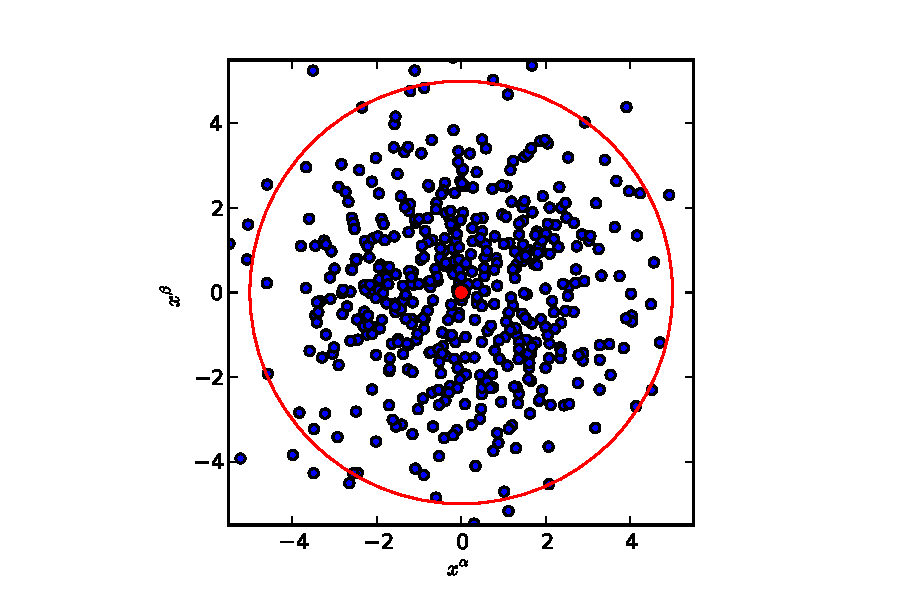
\includegraphics[width=7cm]{figs/fig-1x1.pdf}  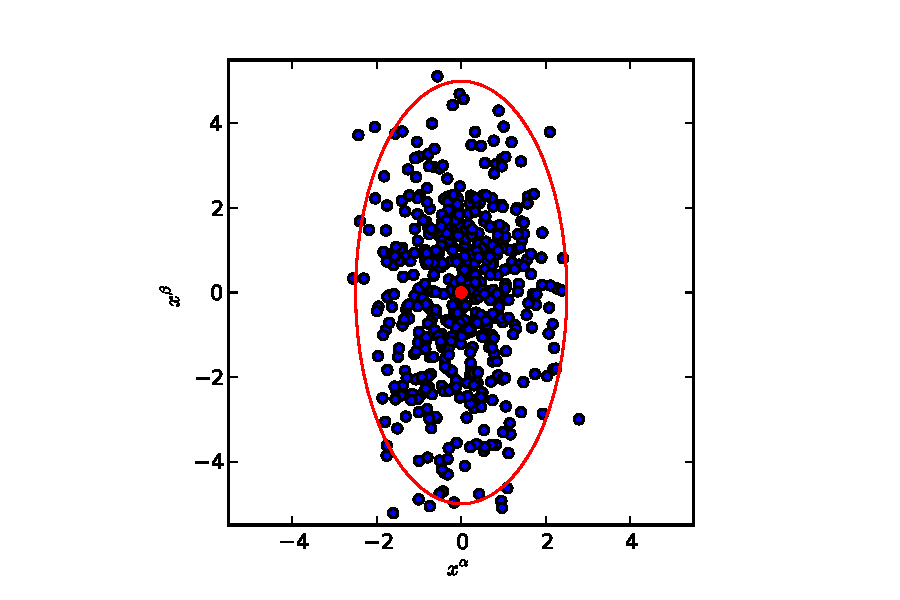
\includegraphics[width=7cm]{figs/fig-1x2.pdf}
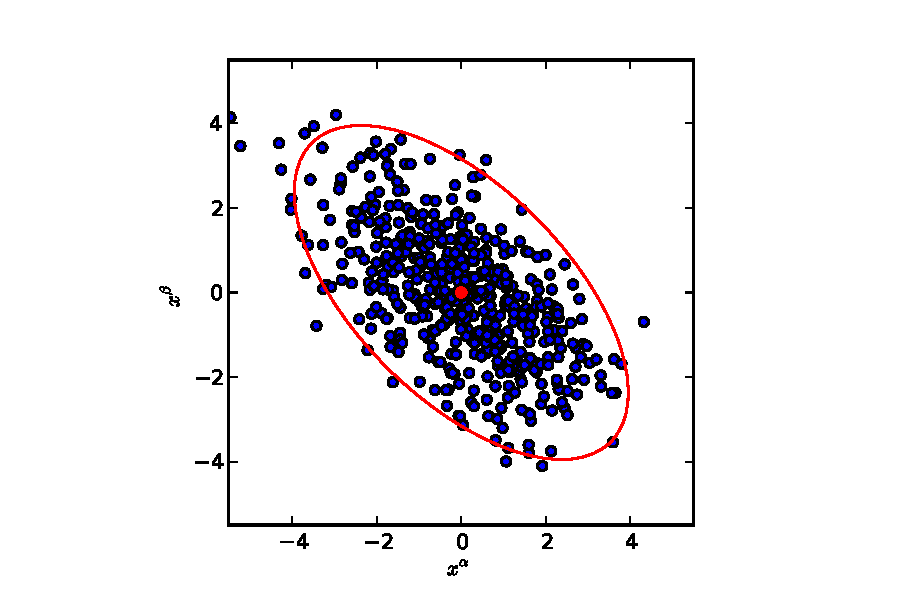
\includegraphics[width=7cm]{figs/fig-1x2rot1.pdf}  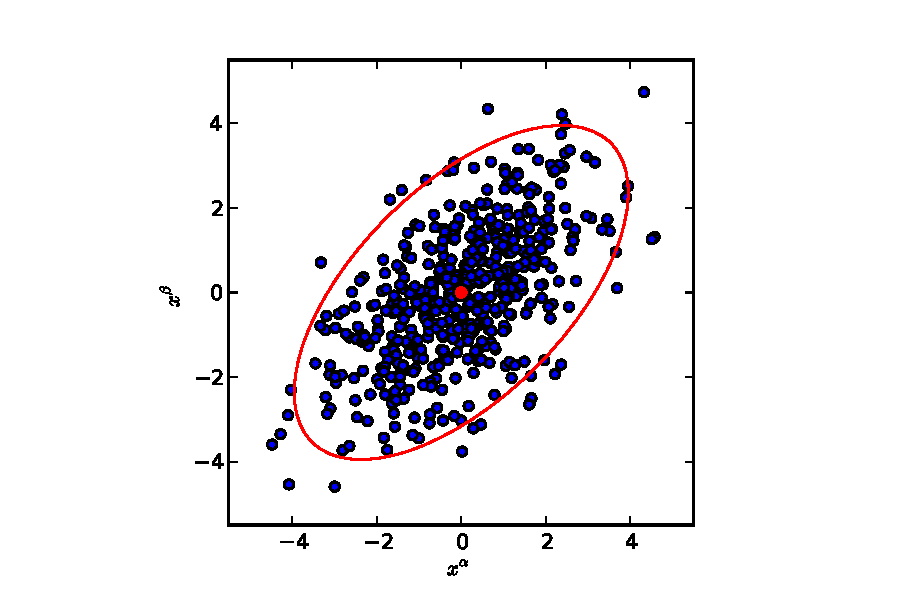
\includegraphics[width=7cm]{figs/fig-1x2rot2.pdf}
\caption{Distribuciones normales bivariadas.}
\end{center}
\label{fig-dist}
\end{figure}

\section{Error en la determinación de parámetros usando MMC}

Para encontrar la incerteza en la estimación de los parámetros $b_0$ y $b_1$ determinados por el MMC ponderado podemos usar el resultado de la sección \ref{sec:propdesv}. Cada punto de nuestros datos, caracterizados por el par $(x_i,y_i$) determina, junto con los errores $\Delta y_i$ determinan los valores de el coeficiente de posición $b_0$ y la pendiente $b_1$ a través de las expresiones \ref{b0MMCP} y \ref{b1MMCP}. Por lo tanto, podemos considerar a $b_0$ como una función particular de las $N$ `variables' $y_i$, donde cada uno de estos valores tiene un error $\Delta y_i$ (estamos ignorando el posible error de $x_i$). Si cada uno de los errores $\Delta y_i$ es la desviación estándar de muchos valores medidos para un correspondiente valor de $x_i$ dado ($\Delta y_i=\sigma_i$), entonces podemos aplicar \ref{pe} para calcular la desviación estándar de $b_0$, usando
\begin{equation}
\sigma_{b_0}^2\approx\sum_{i=1}^N\left(\frac{\partial b_0}{\partial y_i}\right)^2\sigma_i^2.
\end{equation}
A partir de \ref{b0MMCP} encontramos
\begin{equation}
\frac{\partial b_0}{\partial y_i}=\frac{1}{\Delta}\left(\frac{1}{\sigma_i^2}\sum_j\frac{x_j^2}{\sigma_j^2}-\frac{x_i}{\sigma_i^2}\sum_j\frac{x_j}{\sigma_j^2}\right)
\end{equation}
\begin{equation}
\Delta:=\left(\sum_i\frac{1}{\sigma_i^2}\right)\left(\sum_j\frac{x_j^2}{\sigma_j^2}\right)-\left(\sum_i\frac{x_i}{\sigma_i^2}\right)^2.
\end{equation}
Con esto, luego de algo de álgebra, obtenemos
\begin{equation}
\sigma_{b_0}^2\approx \frac{1}{\Delta}\sum_i\frac{x_i^2}{\sigma_i^2}.
\end{equation}
Análogamente, para la pendiente $b_1$, se encuentra
\begin{equation}
\sigma_{b_1}^2\approx \frac{1}{\Delta}\sum_i\frac{1}{\sigma_i^2}.
\end{equation}
Note que en el caso particular en que todos los errores $\sigma_i$ son iguales ($\sigma_i=\sigma$) el MMC ponderado suministra los mismos valores para los coeficientes ajustados, y además
\begin{equation}
\sigma_{b_0}^2\approx \frac{\sigma^2\left(\sum_i x_i^2\right)}{N\left(\sum_i x_i^2\right)-\left(\sum_i x_i\right)^2},
\end{equation}
\begin{equation}
\sigma_{b_1}^2\approx \frac{\sigma^2N}{N\left(\sum_i x_i^2\right)-\left(\sum_i x_i\right)^2}
\end{equation}.
%\paragraph{Ejemplo:}
%Calculemos el 'area de un tri'angulo midiendo diferentes lados y diferentes alturas. Supongamos que disponemos de una regla graduada en mil'imetros y que los diferentes lados y sus correspondientes alturas est'an dadas por: 
%\begin{align}
%a &= (16,09\pm 0,02)\text{ cm}, \qquad h_a= (10,66\pm 0,03)\text{ cm}, \\
%b &= (10,81\pm 0,02)\text{ cm}, \qquad h_b= (15,84\pm 0,03)\text{ cm}, \\
%c &= (17,78\pm 0,02)\text{ cm}, \qquad h_c= (9,66\pm 0,03)\text{ cm}.
%\end{align}
%Para calcular el 'area del tri'angulo rect'angulo debemos utilizar la expresi'on:
%\begin{equation}
%S=\frac{\text{base}\times\text{altura}}{2}.
%\end{equation}
%En general la podemos escribir de la siguiente forma:
%\begin{align}
%S &= \frac{(b\pm\Delta b)(b\pm\Delta b)}{2}=\frac{bh\pm (h\Delta b+b\Delta h)}{2}, \\
%S_a &= (85,7597\pm 0,3478)\text{ cm}^2 \quad \Rightarrow\quad S_a= (85,8\pm 0,4)\text{ cm}^2, \\
%S_b &= (85,6152\pm 0,345)\text{ cm}^2 \quad \Rightarrow\quad S_b= (85,6\pm 0,4)\text{ cm}^2, \\
%S_c &= (85,8774\pm 0,3227)\text{ cm}^2 \quad \Rightarrow\quad S_c= (85,9\pm 0,4)\text{ cm}^2.
%\end{align}
%Los valores son iguales dentro de las imprecisiones experimentales.
%?`Qu'e valor representa mejor el 'area del tri'angulo?
%
%Utilizamos el promedio aritm'etico para encontrar el valor m'as probable
%\begin{align}
%S &= \bar{S}\pm\Delta S, \\
%\bar{S} &=\frac{1}{N}\sum_{i=1}^N S_i=\frac{1}{3}\sum_{i=1}^N S_i=85,8, \\
%\Delta S &= \sqrt{\frac{1}{N}\sum_{i=1}^N (S_i-\bar{S})^2}=\sqrt{\frac{1}{3}\left(0^2+0,2^2+0,1^2\right)}=0,2.
%\end{align}
%Finalmente el resultado queda expresado como:
%\begin{equation}
%\bar{S}=(85,8\pm 0,4)\text{ cm}^2,
%\end{equation}
%donde $0,4$ es el mayor entre el error cuadr'atico medio y la propagaci'on del error asociado a cada 'area. 
%
%
%
%
%
%
%
%Para el caso en que se mida varias veces la misma cantidad y suponiendo
%que los errores asociados a estas medidas se producen por causas
%aleatorias, un buen estimador del error o de la variabilidad del resultado, podría ser la desviación estándar; expresando el resultado de nuestro experimento como
%\begin{equation}
%\bar{x}\pm \Delta x,
%\end{equation}
%donde $\bar{x}$ es el \textbf{promedio} de nuestras medidas y $\Delta x$ es el
%mayor error, entre el error asociado al instrumento y el error
%calculado:
%
%\begin{equation}
%\bar{x}:=\frac{1}{N}\sum_{i=1}^N x_i\qquad \text{(promedio).}
%\end{equation}
%
%\begin{equation}
%s:=\sqrt{\frac{1}{(N-1)}\sum_{i=1}^N(x_i-\bar{x})^2}, \qquad \text{(desviación estándar).}
%\end{equation} 
%
%En este punto es bueno tener presente que existen otros valores medios y otras estimaciones para el error, como:
%\begin{equation}
%x_g:=\sqrt[N]{x_1\cdot x_2\cdots x_N}, \qquad \text{(media geom'etrica)}
%\end{equation}
%
%\begin{equation}
%\frac{1}{x_a}:=\frac{1}{N}\sum_{i=1}^N\frac{1}{x_i}, \qquad \text{(media arm'onica).}
%\end{equation}
%
%Otra medida de tendencia central es la \textbf{mediana}:
%\begin{equation}
%\bar{x}:=\left\lbrace
%		\begin{array}{ll}
%			x_{[(N+1)/2]}, & N \text{ impar} \\
%            \left(x_{[N/2]}+x_{[N/2+1]}\right)/2, & N \text{ par} \\
%        \end{array}\right.
%\end{equation}
%
%\begin{equation}
%s:=\sqrt{\frac{1}{N(N-1)}\sum_{i=1}^N(x_i-\bar{x})^2}, \qquad \text{(error estándar).}
%\end{equation} 
%
\section{Algunos Teoremas}

Ver \url{https://en.wikipedia.org/wiki/Simple_linear_regression}

%\chapter{Series de tiempo}
%\section{Introducci'on}
%
%Una serie de tiempo es una secuencia de observaciones ordenadas cronologicamente y dependientes entre si.
%Ejemplos: Temperatura en Concepci'on, producto interno bruto etc. En los casos mencionados vemos que el valor esta basado en datos anteriores.
%
%Las series de tiempo las podemos clasificar como:
%Discretas: Cuando el conjunto de observaciones es finito o infinito numerable $y_t$.
%
%Continuas: Cuando el conjunto de observaciones es infinito no numerable.
%
%Deterministicas: Cuando se puede usar un modelo para predecir exactamenten los valores futuros de la serie.
%
%Estocasticos: Cuando los valores futuros de la serie s'olo pueden ser determinados en t'erminos probabilisticos, pues el modelo tiene un factor aleatorio.
%
%Una de las caracteristicas especiales de las series de tiempo, es que observaciones sucesivas no son independientes, de modo que su analisi debe considerar el orden de dichas observaciones.
%
%Como objetivo nos plantearemos:
%
%1.- Encontrar un modelo (o familia de modelos) que describa estas series.
%2.- Con el modelofiltrar la se\~nal de ruido, predecir valores futuros y controlar valores futuros.
%
%\section{Componentes de una Serie Temporal}
%
%El an'alisis cl'asico de las series temporales se basa en la suposici'on de que los valores que toma la variable de observaci'on es la consecuencia de tres componentes, cuya acci'on conjunta da como resultado los valores medidos.
%
%Las tres componentes principales son:
%a.- Tendencia $(T_t)$ se puede definir como un cambio de largo plazo y esta relacionado con el cambio de la media. Esta tendencia podr'ia se modelada por regresi'on y los coeficientes ajustados por algunos de los metodos usados (Minimos cuadrados, m'inimos cuadrados ponderados o Maxima verosimilitud)
%
%b.- Componente estacional $(E_t)$ Muchas series de tiempo presentan ciertos variaciones periodicas. Es importante hacer notar que podrian haber 2 o m'as periodos y si un periodo es mucho mayor que el otro, suelen llamar al periodo mayor ciclo.
%Como en muchos casos lo que se busca es determinar la tendencia, la estacionalidad debe ser eliminada del modelo predictor. Este proceso se llama desestacionalizar la serie.
%Ejemplo: El indice de precios al consumidor IPC, en este caso suelo buscarse la tendencia del IPC y no las variaciones estacionales, las cuales se repiten todos los a\~nos en determinados meses y no aportan a conocer la tendecia de largo plazo.
%
%c.- Componete aleatoria $(I_t)$ esta componente no responde a ningun patron de comportamiento, sino que es el resultado de factyores aleatorios que inciden en la serie de tiempo.
%
%Los dos casos m'as simples a ser estudiandos en estos apuntes son:
%
%1.- Si la serie estubiese formada por la suma de las mencionadas componentes.
%
%\begin{equation}
%Y_t=T_t+E_t+I_t
%\end{equation}
%Incluir grafico de la serie como suma
%Incluir graficos de $T_t$ $E_t$ $I_t$
%por separado cada componente
%Filtro
%Media movil
%Ejemplo
%suavizar borrando estacionalidad y ruido para determinar tendencia.
%luego hacer analisis de fourier para encontrar estacionalidad
%analisis de residuos para ver su es realmente ruido o tiene estructura
%Mostrar como caracterizar el ruido unado deferencias
%Graficar ruido hacer historama del ruido
%
%2.- Si la serie estubiese formada por el producto de las componentes.
%\begin{equation}
%Y_t=T_t*E_t*I_t
%\end{equation}
%
%Mostrar el grafico de una serie para este caso
%Graficar cada componente por separado.
%Usar media movil para suavizar la serie
%Usar media movil para borrar estacionalidad
%
%
%Cuando hablamos de una secuencia de valores observados a lo largo del tiempo, la denominamos, en un sentido amplio, \textbf{serie temporal}. Resulta dif'icil imaginar una rama de la ciencia en la que no aparezcan datos que puedan ser considerados como series temporales.
%
%Si, conocidos los valores pasados de la serie, no fuera posible predecir con total certeza el pr'oximo valor de la variable, decimos que la serie es \textbf{no determinista} o \textbf{aleatoria}, y l'ogicamente es de 'estas de las que se ocupa el cuerpo de doctrina denominado ``an'alisis de series temporales'' y al que vamos a dedicar esta breve introducci'on.
%
%El an'alisis estad'istico de series temporales se usa hoy d'ia en muchas 'areas de la Ciencia, fundamentalmente en f'isica, Ingenier'ia y en Econom'ia.
%
%Los objetivos del an'alisis de series temporales son diversos, pudiendo destacar la predicci'on, el control de un proceso, la simulaci'on de procesos, y la generaci'on de nuevas teor'ias f'isicas o biol'ogicas.
%
%Denominamos \textbf{predicci'on} a la estimaci'on de valores futuros de la variable en funci'on del comportamiento pasado de la serie. Este objetivo se emplea ampliamente en el campo de la Ingenier0ia y de la Econom'ia, incluyendo en esta 'ultima rama tambi'en la sanidad p'ublica y la vigilancia de la salud. 
%As'i por ejemplo, la predicci'on mediante modelos basados en la teor'ia de series temporales, puede servir para una buena planificaci'on de recursos sanitarios, en funci'on de la demanda que se espera en el futuro, prevista por el modelo. Otro de los campos en los que se aplica la predicci'on mediante series temporales es el de la meteorolog'ia o en la predicci'on de otros fen'omenos naturales.
%
%En la teor'ia de control de procesos, se trata de seguir la evoluci'on de una variable determinada con el fin de regular su resultado. Esta teor'ia se utiliza en Medicina en los Centros de Control de Enfermedades.
%La \textbf{simulaci'on} se emplea en investigaci'on aplicada, cuando el proceso es muy complejo para ser estudiado de forma anal'itica.
%
%Evidentemente, aunque el valor futuro de una serie temporal no sea predecible con total exactitud, para que tenga inter'es su estudio, el resultado tampoco puede ser completamente aleatorio, existiendo alguna regularidad en cuanto a su comportamiento en el tiempo, lo que har'a posible su modelado y por ende, en su caso, la predicci'on. La b'usqueda de regularidades y de patrones ha sido siempre una de las tareas b'asicas de la Ciencia, y muchas veces se descubren simetr'ias que sirven de fundamento para la predicci'on del comportamiento de los fen'omenos, incluso antes de que se entienda la raz'on o causa que justifica esa regularidad. Esto ocurri'o, por ejemplo, con el sistema peri'odico de los elementos, descrito por Mendeleiev (1834-1907), quien organiz'o de forma muy correcta los elementos qu'imicos en base a las simetr'ias observadas entre ellos, antes de que se comprendiese la raz'on de esas simetr'ias o periodicidad, razones que luego se fundamentaron sobre todo en trabajos de Schr\"0dinger (1887-1961) y Pauli (1900-1958).
%
%Por lo tanto, si podemos encontrar patrones de regularidad en diferentes secciones de una serie temporal, podremos tambi'en describirlas mediante modelos basados en distribuciones de probabilidad. La secuencia ordenada de variables aleatorias $x(t)$ y su distribuci'on de probabilidad asociada, se denomina \textbf{proceso estoc'astico}. Un proceso estoc'astico es por tanto el modelo matem'atico para una serie temporal.
%
%Un concepto importante que encontramos en este 'ambito, es el de procesos estacionarios. Si examinamos por ejemplo la temperatura para un determinado mes a lo largo de los a\~nos en una determinada zona geogr'afica, y se est'a produciendo un cambio clim'atico, aunque haya fluctuaciones, habr'a una tendencia creciente. De una manera informal, diremos que una serie es \L{estacionaria} cuando se encuentra en equilibrio estad'istico, en el sentido de que sus propiedades no var'ian a lo largo del tiempo, y por lo tanto no pueden existir tendencias. Un proceso es \textbf{no-estacionario} si sus propiedades var'ian con el tiempo, como el clima.
%
%Vamos ahora a presentar tres enfoques diferentes, aunque relacionados, para el an'alisis de series temporales.
%
%El primer paso obligatorio para analizar una serie temporal es presentar un Gr'afico de la evoluci'on de la variable a lo largo del tiempo, como puede ser el de la figura \ref{fig-serie1}:
%
%\begin{figure}[h!]
%\begin{center}
%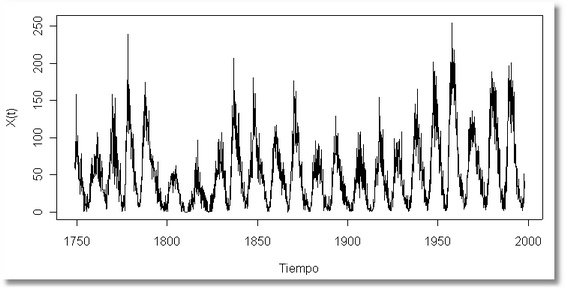
\includegraphics[width=10cm]{figs/i6.png}
%\end{center}
%\caption{Serie temporal.}
%\label{fig-serie1}
%\end{figure}
%
%El siguiente paso consistir'a en determinar si la secuencia de valores es completamente aleatoria o si, por el contrario, se puede encontrar alg'un patr'on a lo largo del tiempo, pues s'olo en este caso podremos seguir con el an'alisis.
%
%La metodolog'aa tradicional para el estudio de series temporales es bastante sencilla de comprender, y fundamentalmente se basa en descomponer las series en varias partes: tendencia, variaci'on estacional o peri'odica, y otras fluctuaciones irregulares.
%
%\paragraph{Tendencia.} Es la direcci'on general de la variable en el periodo de observaci'on, es decir, el cambio a largo plazo de la media de la serie. 
%
%\paragraph{Estacionalidad.} Corresponde a fluctuaciones peri'odicas de la variable, en periodos relativamente cortos de tiempo. 
%
%\paragraph{Otras fluctuaciones irregulares.} Despu'es de extraer de la serie la tendencia y variaciones c'iclicas, nos quedar'a una serie de valores residuales, que pueden ser o no totalmente aleatorios. Volvemos a estar como en el punto de partida, pues ahora tambi'en nos interesa determinar si esa secuencia temporal de valores residuales puede o no ser considerada como aleatoria pura.
%
%En la figura \ref{fig-serie2} vemos un ejemplo de una serie temporal en la que se aprecia la existencia de las distintas componentes comentadas
%\begin{figure}[h!]
%\begin{center}
%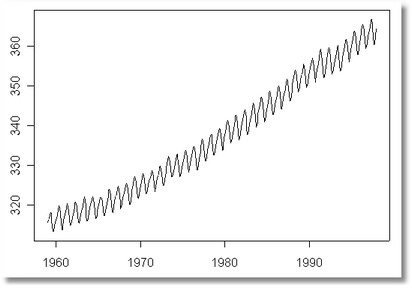
\includegraphics[width=8cm]{figs/i7.png}
%\end{center}
%\caption{Tendencia, estacionalidad y fluctuaciones irregulares.}
%\label{fig-serie2}
%\end{figure}
%
%\section{Componentes de una serie: tendencia, estacionalidad y ruido}
%
%\section{an'alisis de la tendencia}
%Una primera idea sobre la presencia de tendencia en la serie la obtendremos en su representaci'on gr'afica. Pero no siempre estar'a tan clara como en la figura \ref{fig-serie2}. Por ejemplo, en los datos de la figura \ref{fig-serie3} sigue habiendo tendencia, pero ya no es tan marcada.
%\begin{figure}[h!]
%\begin{center}
%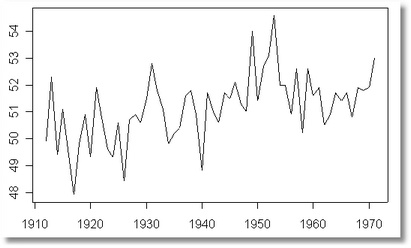
\includegraphics[width=8cm]{figs/i8.png}
%\end{center}
%\caption{Tendencia, estacionalidad y fluctuaciones irregulares.}
%\label{fig-serie3}
%\end{figure}
%
%Los medios m'as utilizados para detectar y eliminar la \textbf{tendencia} de una serie se basan en la aplicaci'on de \textbf{filtros} a los datos. Un filtro no es m'as que una funci'on matem'atica que aplicada a los valores de la serie produce una nueva serie con unas caracter'isticas determinadas. Entre esos filtros encontramos las \textbf{medias m'oviles}. 
%
%Una media m'ovil se calcula, para cada punto, como un promedio del mismo n'umero de valores a cada lado de ese punto. as'i una media m'ovil de tres puntos se calcula como:
%\begin{equation}
%m(x_t)=\frac{x_{t-1}+x_t+x_{t+1}}{3}.
%\end{equation}
%Mientras que una media m'ovil de cuatro puntos viene dada por
%\begin{equation}
%m(x_t)=\frac{x_{t-2}/2+x_{t-1}+x_t+x_{t+1}+x_{t+2}/2}{4}.
%\end{equation}
%
%Cuando la cantidad de puntos de la media m'ovil es par, se toma la mitad de los valores extremos.
%
%Existen otros procedimientos para extraer la tendencia, como \textbf{ajuste de polinomios}, entre otros. 
%
%Una clase de filtro, que es particularmente 'util para eliminar la tendencia, se basa en aplicar \textbf{diferencias} a la serie hasta convertirla en estacionaria. Una diferencia de primer orden se obtiene restando dos valores contiguos:
%\begin{equation}
%\Delta x_{t+1}:=x_{t+1}-x_t.
%\end{equation}
%Si volvemos a diferenciar esa serie, restando los nuevos valores consecutivos obtenemos una nueva serie m'as suavizada.
%\begin{equation}
%\Delta^2 x_{t+2}:=\Delta x_{t+2}-\Delta x_{t+1}.
%\end{equation}
%
%Una vez que se aplica un proceso cl'asico de descomposici'on mediante un procedimiento de medias m'oviles a los datos de la figura \ref{fig-serie2}, se obtiene las siguientes series:
%\begin{figure}[h!]
%\begin{center}
%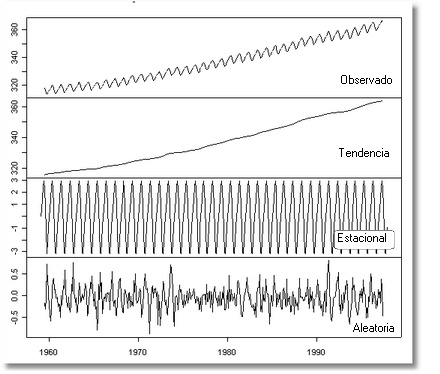
\includegraphics[width=8cm]{figs/i10.png}
%\end{center}
%\caption{Observado, tendencia, estacional, aleatoria.}
%\label{fig-serie4}
%\end{figure}
%
%Para analizar la \textbf{estacionalidad} de una serie introduciremos un concepto de gran inter'es en el an'alisis de series temporales: la \textbf{funci'on de autocorrelaci'on}. 
%
%La \textbf{funci'on de autocorrelaci'on} mide la correlaci'on entre los valores de la serie distanciados un lapso de tiempo $k$.
%
%La f'ormula del coeficiente de correlaci'on simple, dados $N$ pares de observaciones $y$, $x$:
%\begin{equation}
%r:=\frac{\sum (y_i-\bar{y})(x_i-\bar{x})}{\sqrt{\sum(y_i-\bar{y})^2\sum(x_i-\bar{x})^2}}.
%\end{equation}
%
%De igual forma, dada una secuencia temporal de $N$ observaciones $x_1,\cdots,x_N$, podemos formar $N-1$ parejas de observaciones contiguas $(x_1, x_2), (x_2,x_3),\cdots (x_{N-1},x_N)$ y calcular el coeficiente de correlaci'on de estas parejas. 
%
%A este coeficiente lo denominaremos \textbf{coeficiente de autocorrelaci'on} de orden 1 y lo denotamos como $r1$. An'alogamente se pueden formar parejas con puntos separados por una distancia $2$, es decir $(x_1,x_3), (x_2,x_4)$,  etc. y calcular el nuevo coeficiente de autocorrelaci'on de orden 2. De forma general, si preparamos parejas con puntos separados una distancia $k$, calcularemos el coeficiente de autocorrelaci'on de orden $k$.
%
%Al igual que para el coeficiente de correlaci'on lineal simple, se puede calcular un error est'andar y por tanto un intervalo de confianza para el coeficiente de autocorrelaci'on.
%
%La \textbf{funci'on de autocorrelaci'on} es el conjunto de coeficientes de autocorrelaci'on $rk$ desde 1 hasta un m'aximo que no puede exceder la mitad de los valores observados, y es de gran importancia para estudiar la estacionalidad de la serie, ya que si 'esta existe, los valores separados entre s'i por intervalos iguales al periodo estacional deben estar correlacionados de alguna forma. Es decir que el coeficiente de autocorrelaci'on para un retardo igual al periodo estacional debe ser significativamente diferente de 0.
%
%\section{m'etodos de an'alisis de componentes}

\begin{thebibliography}{99}
\bibitem{CODATA2010} Mohr \textit{et al.}, {\sl Rev. Mod. Phys.} {\bf 84}, 1527 (2012) \url{http://dx.doi.org/10.1103/RevModPhys.84.1527}.

\bibitem{HH2010} I.G. Hughes and T.P.A. Hase, \textit{Measurements and their Uncertainties: A practical guide to modern error analysis}, Oxford University Press (2010).
\end{thebibliography}

\end{document}

